\documentclass[twoside]{book}
\usepackage[normalem]{ulem}
\usepackage[12pt]{extsizes}
\usepackage[utf8]{inputenc}
\usepackage[T2A]{fontenc}
\usepackage{amsmath}
\usepackage{amssymb}
\usepackage{mathtools}
\usepackage{hyperref}
\usepackage{mathdots}
\usepackage{amsfonts}
\usepackage{bbold}
\usepackage{cmap}
\usepackage{multicol}
\usepackage{comment}
\usepackage[parfill]{parskip}
\usepackage{enumitem}
\usepackage{longtable}
\usepackage{varwidth}

\usepackage{listings}
\usepackage{color}
\usepackage{colortbl}
\usepackage{xcolor}
\usepackage[left=1.5cm,right=2cm,top=2cm,bottom=2cm,bindingoffset=0.1cm]{geometry}
\usepackage[russian]{babel}
\usepackage[pdf]{graphviz}
\usepackage{tikz}

\usepackage{etoolbox}
\AtBeginEnvironment{enumerate}{\linespread{.84}\selectfont}
\newcommand{\ctd}{\begin{flushright} \(\square\) \end{flushright}}

\usepackage{graphicx}
\setlength\fboxsep{3pt}
\setlength\fboxrule{1pt}

\hypersetup{
    colorlinks=true,
    linkcolor=blue,
    filecolor=magenta,      
    urlcolor=blue,
    pdftitle={Alfo},
    pdfpagemode=FullScreen,
}
\newcommand{\updownarrows}{\mathbin\uparrow\hspace{-.5em}\downarrow}
\newcommand{\downuparrows}{\mathbin\downarrow\hspace{-.5em}\uparrow}
\newcommand{\defeq}{\overset{\mathrm{def}}{=\joinrel=}}
\newcommand{\defLeftrightarrow}{\xLeftrightarrow{def}}
\newcommand{\skewed}{\mathrel{\raisebox{3pt}{\(\underline{\,\cdot\,}\)}}}

\makeatletter
\renewcommand*\env@matrix[1][*\c@MaxMatrixCols c]{%
  \hskip -\arraycolsep
  \let\@ifnextchar\new@ifnextchar
  \array{#1}}
\makeatother

\DeclareMathOperator{\proj}{proj}
\DeclareMathOperator{\rg}{rg}
\DeclareMathOperator{\spann}{span}
\DeclareMathOperator{\inv}{inv}
\newcommand{\mytilde}{\raisebox{0.5ex}{\texttildelow}}
\newcommand{\deff}[1]{\underline{\textbf{#1}}}
\newcommand{\thmm}[1]{\underline{\textbf{#1}}}
\newcommand{\prooff}[1]{{\underline{Доказательство:}} \\ }

\title{\Huge Линейная алгебра}
\author{Леонид Альжанов, Вячеслав Чепелин и другие}
\date{ }

\begin{document}
\maketitle
\tableofcontents

\chapter{Аналитическая геометрия}
\section{Элементы векторной алгебры}
\subsection{Основные определения}
\(V\) --- пространство геометрических векторов.

Геометрический (свободный) вектор \(\vec a\) --- направленный отрезок в пространстве.

Длина (модуль) вектора \(|\vec a| = |\overrightarrow{AB}| = AB\) --- длина отрезка, на котором строится вектор.

Нулевой вектор \(\vec 0\) --- имеет длину ноль, начало совпадает с концом.

Вектор независим от точки приложения (его начала)

\(\vec a \parallel \vec b \defLeftrightarrow\) они лежат на одной или параллельных прямых

\(\forall \vec a:\vec 0 \parallel \vec a\)

\(\upuparrows\) и \(\updownarrows\) --- обозначение сонаправленности и разнонаправленности векторов.

\(
\vec a = \vec b\ \defLeftrightarrow
\begin{cases*}
    \vec a \upuparrows \vec b \\
    |\vec a| = |\vec b|       \\
\end{cases*}
\)

\(\vec a, \vec b, \vec c\) - компланарны \(\defLeftrightarrow\) лежат или параллельны одной плоскости.

\(\vec a_0\) --- орт вектор вектора \(\vec a \defLeftrightarrow\)
\(
\begin{cases*}
    \vec a_0 \upuparrows \vec a \\
    |\vec a_0| = 1              \\
\end{cases*}
\)

Вектора можно складывать: \(\vec a + \vec b = \vec c\). Строится по правилу треугольника или параллелограмма.

Вектора можно умножать на скаляр: \(\vec c = \vec a \cdot \lambda, \lambda \in \mathbb R\).
\begin{itemize}
    \item[] \(|\vec c| = |\vec a| \cdot |\lambda|\)
    \item[] \(\lambda > 0: \vec a \upuparrows \vec c\)
    \item[] \(\lambda < 0: \vec a \updownarrows \vec c\)
    \item[] \(\lambda = 0: \vec c = \vec 0\)
\end{itemize}
Вектора можно вычитать: \(\vec a - \vec b = \vec a + (-1) \cdot \vec b = \vec c\).

У \((V, ``+" \,, ``\cdot \lambda")\) есть свойства:
\begin{enumerate}
    \item \(\forall \vec a, \vec b: \vec a + \vec b = \vec b + \vec a\)
    \item \(\forall \vec a, \vec b, \vec c: (\vec a + \vec b) + \vec c = \vec a + (\vec b + \vec c)\)
    \item \(\exists \vec 0: \forall \vec a: \vec a + \vec0 = \vec a\)
    \item \(\forall \vec a: \exists (- \vec a): \vec a+(- \vec a) = \vec 0\)
    \item \(\forall \lambda \in \mathbb R: \forall \vec a, \vec b: \lambda (\vec a + \vec b) = \lambda \vec a + \lambda \vec b\)
    \item \(\forall \lambda, \mu \in \mathbb R: \forall \vec a: (\lambda + \mu)\vec a = \lambda \vec a + \mu \vec a\)
    \item \(\forall \lambda, \mu \in \mathbb R: \forall \vec a: (\lambda \mu)\vec a = \mu(\lambda \vec a)\)
    \item \(\forall \vec a: 1 \cdot \vec a = \vec a\)
\end{enumerate}

Вcё это доказывается из школьной геометрии. Эти свойства (аксиомы) линейного пространства \(\Rightarrow (V, ``+" \,, ``\cdot \lambda")\) --- линейное пространство.

\(
\begin{rcases*}
    \vec v_1, \vec v_2, \dots, \vec v_n \in V
    \lambda_1, \lambda_2, \dots, \lambda_n
\end{rcases*}
\Rightarrow \sum\limits_{i = 1}^{n} \lambda_i \vec v_i = \vec v\) --- линейная комбинация векторов \(\vec v_1, \vec v_2, \dots, \vec v_n\), или \(\vec v\) разложен по векторам \(\vec v_1, \vec v_2, \dots, \vec v_n\).

\(\sum\limits_{i = 1}^{n} \lambda_i \vec v_i = \vec 0\) --- нулевая линейная комбинация.

Линейная комбинация --- тривиальная \(\defLeftrightarrow \forall i \in \{1, \dots, n\}: \lambda_i = 0\)

Система векторов \(\vec v_1, \vec v_2, \dots, \vec v_n\) --- линейно независимая \(\defLeftrightarrow\) все её нулевые линейные комбинации --- тривиальные. То есть система векторов \(\vec v_1, \vec v_2, \dots, \vec v_n\) --- линейно независимая \(\defLeftrightarrow \sum\limits_{i = 1}^{n} \lambda_i \vec v_i = \vec 0 \Leftrightarrow \forall i \in \{1, \dots, n\}: \lambda_i = 0\). Пример: \(\forall a, b : a \nparallel b\)

Система векторов \(\vec v_1, \vec v_2, \dots, \vec v_n\) --- линейно зависимая \(\defLeftrightarrow\) существует её нулевая нетривиальная линейная комбинация. То есть система векторов \(\vec v_1, \vec v_2, \dots, \vec v_n\) --- линейно зависимая \(\defLeftrightarrow \exists \lambda_i \neq 0:\sum\limits_{i = 1}^{n} \lambda_i \vec v_i = \vec 0\). Пример: \(\forall a, b : a \parallel b\)

Свойства линейной зависимости:
\begin{enumerate}
    \item \(\vec 0 \in \{\vec v_1, \vec v_2, \dots, \vec v_n\} \Rightarrow \vec v_1, \vec v_2, \dots, \vec v_n\) --- линейно зависимая система.

          Пусть \(\vec v_k = \vec 0\). Возьмём \(\lambda_k = 1\), а \(\forall i \neq k: \lambda_i = 0\). Значит \(\sum\limits_{i = 1}^{n} \lambda_i \vec v_i = 0 \vec v_1 + 0 \vec v_2 + \dots + 1 \vec v_k + \dots + 0 \vec v_n = 1 \cdot \vec 0 = \vec 0 \quad Q.E.D\)

    \item \(\vec v_1, \vec v_2, \dots, \vec v_n\) --- линейно зависимая система \(\Rightarrow \vec v_1, \vec v_2, \dots, \vec v_n, \vec v_{n + 1}, \vec v_{n + 2}, \dots \vec v_{n + m}\) --- линейно зависимая система.

          Возьмём \(\lambda_1, \lambda_2, \dots, \lambda_n\), создающие нулевую нетривиальную линейную комбинацию, а \(\forall i \in \{n + 1, n + 2, \dots, n + m\}\) возьмём \(\lambda_i = 0\). Тогда \(\sum\limits_{i = 1}^{n + m} \lambda_i \vec v_i = \sum\limits_{i = 1}^{n} \lambda_i \vec v_i = 0 \vec v_{n + 1} + 0 \vec v_{n + 2} + \dots + 0 \vec v_{n + m} = \vec 0 + \vec 0 = \vec 0 \quad Q.E.D\)\\

    \item В линейно зависимой системе \(\vec v_1, \vec v_2, \dots, \vec v_n\) есть вектор, который можно выразить линейной комбинацией других, то есть \(\exists \vec v_k: v_k = \sum\limits_{i = 1, i \neq k}^{n} \mu_i \vec v_i\).

          Возьмём \(\lambda_1, \lambda_2, \dots, \lambda_n\), создающие нулевую нетривиальную линейную комбинацию \(\Rightarrow \exists \lambda_k \neq 0 \Rightarrow \lambda_k \vec v_k = \sum\limits_{i = 1, i \neq k}^{n} \lambda_i \vec v_i \Rightarrow\) возьмём \(\mu_i = \frac{\lambda_i}{\lambda_k} \Rightarrow v_k = \sum\limits_{i = 1, i \neq k}^{n} \mu_i \vec v_i \quad Q.E.D\)

\end{enumerate}

Базис прямой --- любой ненулевой вектор на этой прямой.

Базис плоскости --- любая упорядоченная пара неколлинеарных векторов в данной плоскости.
Базис пространства --- любая упорядоченная тройка некомпланарных векторов в этом пространстве.

\(\vec e_1, \vec e_2, \vec e_3\) --- базис пространства.

\(\vec x = \sum\limits_{i = 1}^{3} \vec e_i x_i, x_i \in \mathbb{R} \Rightarrow (x_1, x_2, x_3)\) --- координаты \(\vec x\) относительно базиса \(\vec e_1, \vec e_2, \vec e_3\). Аналогично для плоскости и прямой.

\begin{enumerate}
    \item \(\forall \vec x \parallel L \; \exists! x_1 \in \mathbb{R}: \vec x = x_1 \vec e_1\), где \(\vec e_1\) --- базис \(L\).

          Пусть \(O \in L\). Приложим к \(O\) начала векторов \(\vec x\) и \(\vec e_1\). \(\vec x \parallel \vec e_1 \Leftrightarrow \exists! x \in \mathbb{R}: \vec x = x_1 \vec e_1\) \(Q.E.D.\)
          \begin{itemize}
              \item[] \(\vec e_1 \upuparrows \vec x: x_1 > 0\)\\
              \item[] \(\vec e_1 \updownarrows \vec x: x_1 < 0\)\\
              \item[] \(\vec x = \vec 0: x_1 = 0\)\\
          \end{itemize}

    \item \(\forall \vec x \parallel \alpha \; \exists! x_1, x_2 \in \mathbb{R}: \vec x = x_1 \vec e_1 + x_2 \vec e_2\), где \(\vec e_1, \vec e_2\) --- базис \(\alpha\).

          Аналогично, пусть \(O \in \alpha\). Приложим к \(O\) начала векторов \(\vec x, \vec e_1\) и \(\vec e_2\). \(\vec x = \vec 0: \vec x = 0 \vec e_1 + 0 \vec e_2\).

          \(\vec x \neq \vec 0:\) пусть \(B\) --- конец \(\vec x\). Проведём \(L_2 \parallel \vec e_2, B \in L_2\).

          Проведём \(L_1 \parallel \vec e_1, O \in L_1\). \(A = L_1 \cap L_2\). \(\vec x = \overrightarrow{OB} = \overrightarrow{OA} + \overrightarrow{AB}\).

          \(
          \begin{rcases*}
              \overrightarrow{OA} \parallel \vec e_1 \Rightarrow (\text{по пункту 1}) \Rightarrow \exists! x_1 \in \mathbb{R}: \overrightarrow{OA} = x_1 \vec e_1 \\
              \overrightarrow{AB} \parallel \vec e_2 \Rightarrow (\text{по пункту 1}) \Rightarrow \exists! x_2 \in \mathbb{R}: \overrightarrow{AB} = x_2 \vec e_2
          \end{rcases*}
          \Rightarrow \vec x = x_1 \vec e_1 + x_2 \vec e_2\) \(Q.E.D.\)

    \item \(\forall \vec x \in V \; \exists! x_1, x_2, x_3 \in \mathbb{R}: \vec x = x_1 \vec e_1 + x_2 \vec e_2 + x_3 \vec e_3\), где \(\vec e_1, \vec e_2, \vec e_3\) --- базис \(V\).

          Пусть \(O \in V\). Приложим к \(O\) начала векторов \(\vec x, \vec e_1, \vec e_2\) и \(\vec e_3\). \(\alpha(O, \vec e_1, \vec e_2)\). \(\vec x = \vec 0: \vec x = 0 \vec e_1 + 0 \vec e_2 + 0 \vec e_3\). \(\vec x \neq \vec 0:\) пусть \(B\) --- конец \(\vec x\). Проведём \(L \parallel \vec e_3, B \in L\). \(A = L \cap \alpha\). \(\vec x = \overrightarrow{OB} = \overrightarrow{OA} + \overrightarrow{AB}\).

          \(
          \begin{rcases*}
              \overrightarrow{OA} \parallel \vec \alpha \Rightarrow (\text{по пункту 2}) \Rightarrow \exists! x_1, x_2 \in \mathbb{R}: \overrightarrow{OA} = x_1 \vec e_1 + x_2 \vec e_2 \\
              \overrightarrow{AB} \parallel \vec e_3 \Rightarrow (\text{по пункту 1}) \Rightarrow \exists! x_3 \in \mathbb{R}: \overrightarrow{AB} = x_3 \vec e_3
          \end{rcases*}
          \Rightarrow \vec x = x_1 \vec e_1 + x_2 \vec e_2 + x_3 \vec e_3\) \(Q.E.D.\)
\end{enumerate}

То есть, любой вектор может быть разложен по базису, и единственным образом.

Следствия:
\begin{enumerate}
    \item \(\vec a = \sum\limits_{i = 1}^{3} a_i \vec e_i, \vec b = \sum\limits_{i = 1}^{3} b_i \vec e_i: \vec a = \vec b \Leftrightarrow \forall i \in \{1, 2, 3\}: a_i = b_i\)

    \item \(\vec a + \vec b = \vec c = \sum\limits_{i = 1}^{3} c_i \vec e_i \Leftrightarrow \forall i \in \{1, 2, 3\}: c_i = a_i + b_i\)

          \(\vec c = \vec a + \vec b = \sum\limits_{i = 1}^{3} a_i \vec e_i + \sum\limits_{i = 1}^{3} b_i \vec e_i = \sum\limits_{i = 1}^{3} (a_i + b_i) \vec e_i = \sum\limits_{i = 1}^{3} c_i \vec e_i \Leftrightarrow \forall i \in \{1, 2, 3\}: c_i = a_i + b_i\) \(Q.E.D.\)

    \item \(\lambda \vec a = \vec c = \sum\limits_{i = 1}^{3} c_i \vec e_i \Leftrightarrow \forall i \in \{1, 2, 3\}: c_i = \lambda a_i\)

          \(\vec c = \lambda \vec a = \lambda \sum\limits_{i = 1}^{3} a_i \vec e_i = \sum\limits_{i = 1}^{3} (\lambda a_i) \vec e_i = \sum\limits_{i = 1}^{3} c_i \vec e_i \Leftrightarrow \forall i \in \{1, 2, 3\}: c_i = \lambda a_i\) \(Q.E.D.\)

\end{enumerate}

\(\vec a \parallel \vec b \Leftrightarrow \exists \lambda \in \mathbb{R}:
\left[
\begin{array}{ll}
    \vec a = \lambda \vec b \\
    \vec b = \lambda \vec a
\end{array}
\right .
\Leftrightarrow
\forall i \in \{1, 2, 3\}:
\left[
\begin{array}{ll}
    a_i = \lambda b_i \\
    b_i = \lambda a_i
\end{array}
\right .
\Leftrightarrow \frac{a_1}{b_1} = \frac{a_2}{b_2} = \frac{a_3}{b_3} = \lambda\) --- коэффициент пропорциональности.

\(\vec v_1, \vec v_2, \vec v_3, \dots, \vec v_n\) --- коллинеарны \(\Rightarrow\) они линейно зависимы в пространстве. Если они коллинеарны, то очевидно. Если \(\exists \vec e_1 \parallel \vec e_2 \in \{\vec v_1, \vec v_2, \dots, \vec v_n\}\), то мы можем выразить остальные вектора в \(\vec v_1, \vec v_2, \dots, \vec v_n\) через \(\vec e_1\) и \(\vec e_2\) \(\Rightarrow \vec v_1, \vec v_2, \dots, \vec v_n\) --- они линейно зависимы в пространстве \(Q.E.D.\)


\subsection{Система координат на плоскости и в пространстве}

Говорят, что в пространстве введена декартова система координат (ДСК), если зафиксирована \((\cdot) O \)(начало координат) и базис \(\vec{e}_1, \vec{e}_2, \vec{e}_3\)

Осями координат называются прямые, содержащие базисные вектора.

\(Ox\) - абсцисс, \(Oy\) - ординат, \(Oz\) - аппликат

Координатами точки \(M\) в ДСК \((O, \vec{e_1}, \vec{e_2}, \vec{e_3})\) называются координаты вектора \(\vec{OM}\) в базисе \((\vec{e_1}, \vec{e_2}, \vec{e_3})\).

Даны 2 точки: \(A(a_1, a_2, a_3), B(b_1, b_2, b_3)\). Тогда \(\overrightarrow{AB} = (b_1-a_1,b_2-a_2,b_3-a_3)\)

Задача: Даны 2 точки: \(A(a_1, a_2, a_3), B(b_1, b_2, b_3)\) и точка \(M = (m_1, m_2, m_3)\), делящая отрезок AB с \(\frac{AM}{MB}=\lambda > 0\). Найти координаты точки \(M\) через \(A, B, \lambda\).

\(AM = \lambda MB \Leftrightarrow |\vec{AM}| = \lambda |\vec{MB}| \Rightarrow \vec{AM} = \lambda \vec{MB}\)

\(m_i - a_i = \lambda (b_i - m_i) \Leftrightarrow m_i = \frac{\lambda b_i + a_i}{1 + \lambda}\)

В дальнейшем будем работать с ортогональной д.к.с., где \(\vec{e_1},\vec{e_2},\vec{e_3}\) попарно ортоганальны и нормированны \((|e_i|=1)\).

Длина вектора в ортонормированной декартовой системе координат равна квадратному корню суммы квадратов координат.

В трёхмерном пространстве сумма квадратов косинусов углов между радиус-вектором точки и осями координат равна единице.

Пусть точка имеет координаты \((x,y,z)\) и располагается на расстоянии \(R\) от центра координат. Тогда \(x^2 + y^2 +z^2 = R^2\), что значит, что \(\left(\frac{x}{R}\right)^2 + \left(\frac{y}{R}\right)^2 + \left(\frac{z}{R}\right)^2 = 1\). Заметим, что \(\frac{x}{R}\) --- это косинус между радиус-вектором точки и осью \(Ox\).

Полярная система координат --- это точка и луч, исходящий из неё, на плоскости. При этом координатами являются расстояние от точки и угол против часовой стрелке от полярного луча до радиус-вектора точки. У точки ноль нет полярных координат, считают, что у нее \(r=0\).

Связь между декартовыми и полярными координатами. Обычно ДСК связывают с ПСК так: центр общий, а полярный луч --- положительное направление \(Ox\). Тогда \(x=r\cos\varphi, y=r\sin\varphi\). Обратно: \(r=\sqrt{x^2 + y^2}, \varphi=\arctan\frac{y}{x} + \pi k\) (неодназначно какой именно точке, надо смотреть в какой четверти точка)

Лемниската Бернулли

$(x^2+y^2)^2=x^2-y^2$. Но приведя в п.с.к:  \(r^4=r^2(\cos^2x-\sin^2x)\leftrightarrow r=\sqrt{\cos(2x)}\). В такой форме можно нарисовать эскиз графика:
\begin{center}
    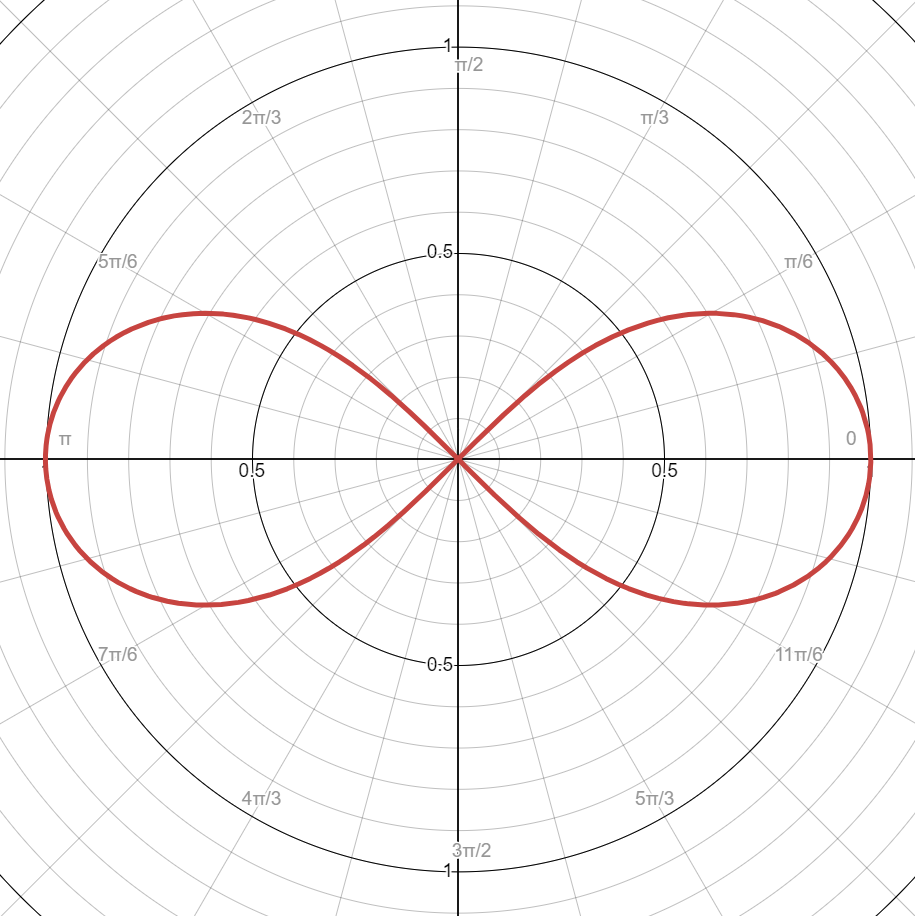
\includegraphics[height=7cm]{Images/Chapter_1/1-2-1.png}
\end{center}


\subsection{Преобразования в ДСК}
\begin{enumerate}[label=\alph*)]
    \item Параллельный перенос
          \begin{center}
              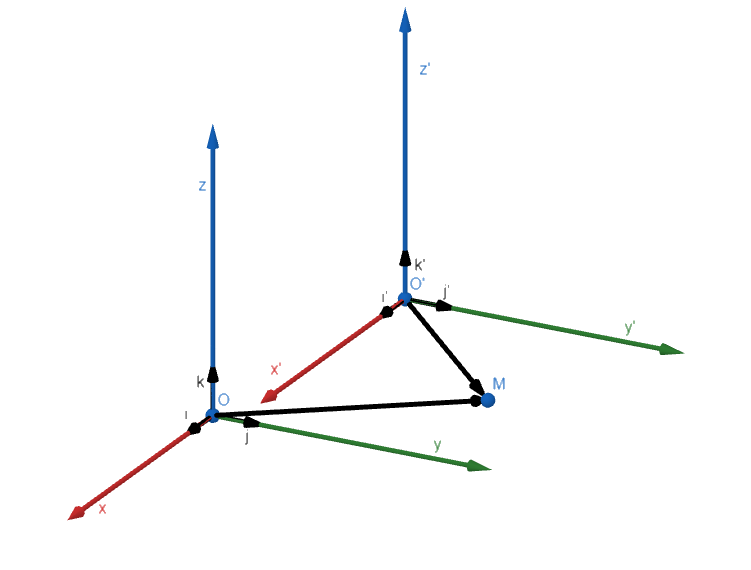
\includegraphics[height=7cm]{Images/Chapter_1/1-3-1.png}
          \end{center}
          Создадим новую ДСК с центром в \(O' = (x_0, y_0, z_0)\).

          \(M = (x, y, z) \text{(в старой)} = (x', y', z') \text{(в новой)} = (x_0 + x', y_0 + y', z_0 + z') \text{(в старой)}\)
    \item Поворот
          \begin{itemize}
              \item На плоскости:
                    \begin{center}
                        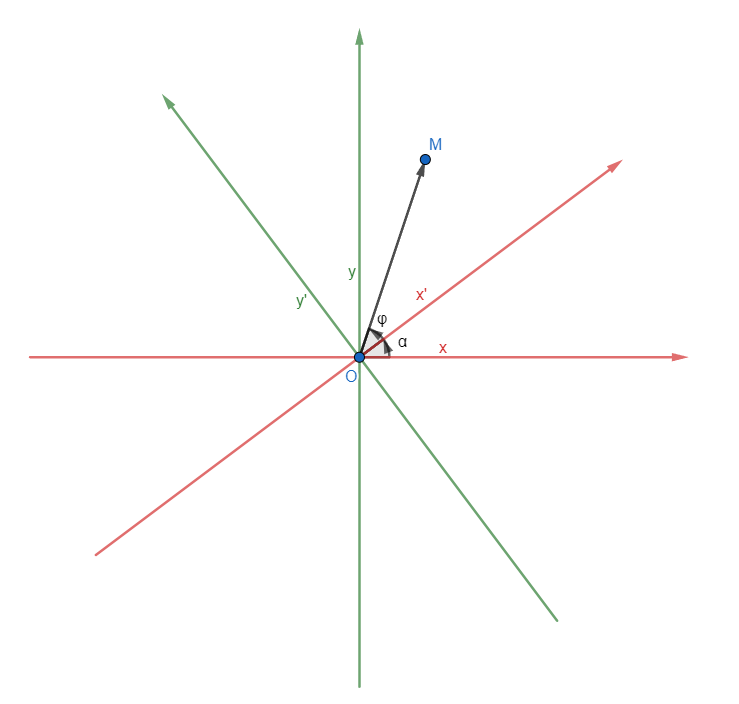
\includegraphics[height=7cm]{Images/Chapter_1/1-3-2.png}
                    \end{center}
                    Создадим новую ДСК, повёрнутую на \(\alpha\).

                    \(M = (x, y) = (r \cos(\varphi + \alpha), r \sin(\varphi + \alpha)) =
                    (x' \cos\alpha - y' \sin\alpha, x' \sin\alpha + y' \cos\alpha)\)

                    \(\begin{pmatrix}
                        x \\
                        y
                    \end{pmatrix} =
                    \begin{pmatrix}
                        \cos\alpha & -\sin\alpha \\
                        \sin\alpha & \cos\alpha
                    \end{pmatrix}
                    \begin{pmatrix}
                        x' \\
                        y'
                    \end{pmatrix}\)

                    \(\begin{pmatrix}
                        x' \\
                        y'
                    \end{pmatrix} =
                    \begin{pmatrix}
                        \cos\alpha  & \sin\alpha \\
                        -\sin\alpha & \cos\alpha
                    \end{pmatrix}
                    \begin{pmatrix}
                        x \\
                        y
                    \end{pmatrix}\)

                    \(\begin{pmatrix}
                        \cos\alpha  & \sin\alpha \\
                        -\sin\alpha & \cos\alpha
                    \end{pmatrix}\) --- Матрица поворота.
              \item В пространстве:
                    \begin{center}
                        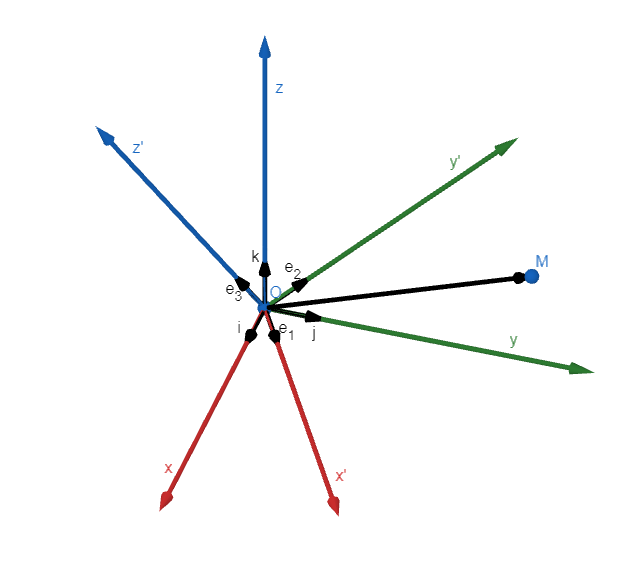
\includegraphics[height=7cm]{Images/Chapter_1/1-3-3.png}
                    \end{center}
                    Создадим новую ДСК, повёрнутую в пространстве.
                    Базис \(\vec i, \vec j, \vec k \rightarrow \vec e_1, \vec e_2, \vec e_3\).
                    Оси \(x, y, z \rightarrow x', y', z'\). Оба базиса попарно ортогональны и нормированы.

                    \(m = 1, 2, 3: \vec e_m = (\cos\alpha_m, \cos\beta_m, \cos\gamma_m)\) - направляющие косинусы.

                    \(M = (x, y, z) = x\vec i + y\vec j + z\vec k = \\
                    = x'(\cos\alpha_1\vec i + \cos\beta_1\vec j + \cos\gamma_1\vec k) + \\
                    + y'(\cos\alpha_2\vec i + \cos\beta_2\vec j + \cos\gamma_2\vec k) + \\
                    + z'(\cos\alpha_3\vec i + \cos\beta_3\vec j + \cos\gamma_3\vec k) = \\
                    = \vec i(x'\cos\alpha_1 + y'\cos\alpha_2 + z'\cos\alpha_3) + \\
                    + \vec j(x'\cos\beta_1 + y'\cos\beta_2 + z'\cos\beta_3) + \\
                    + \vec k(x'\cos\gamma_1 + y'\cos\gamma_2 + z'\cos\gamma_3)\)

                    Т.к. координаты точки задаются единственным способом, то:

                    \(\begin{cases*}
                        x = x'\cos\alpha_1 + y'\cos\alpha_2 + z'\cos\alpha_3 \\
                        y = x'\cos\beta_1 + y'\cos\beta_2 + z'\cos\beta_3    \\
                        z = x'\cos\gamma_1 + y'\cos\gamma_2 + z'\cos\gamma_3
                    \end{cases*}\)

                    \(\begin{pmatrix}
                        x \\
                        y \\
                        z
                    \end{pmatrix} =
                    \begin{pmatrix}
                        \cos\alpha_1 & \cos\alpha_2 & \cos\alpha_3 \\
                        \cos\beta_1  & \cos\beta_2  & \cos\beta_3  \\
                        \cos\gamma_1 & \cos\gamma_2 & \cos\gamma_3
                    \end{pmatrix}
                    \begin{pmatrix}
                        x' \\
                        y' \\
                        z'
                    \end{pmatrix}\)

                    Столбцы в этой матрице - координаты \(\vec e_1, \vec e_2, \vec e_3\).
          \end{itemize}
\end{enumerate}

\subsection{Скалярное произведение векторов}

\(``\cdot": V_3 \times V_3 \rightarrow \mathbb{R}\)

\(\vec a, \vec b \in V_3 \rightarrow (\vec a, \vec b) = \vec a \cdot \vec b \in \mathbb{R}\)

\(\vec a \cdot \vec b = |\vec a| |\vec b| \cos\varphi;\; \varphi = \angle(\vec a, \vec b)\)
\begin{center}
    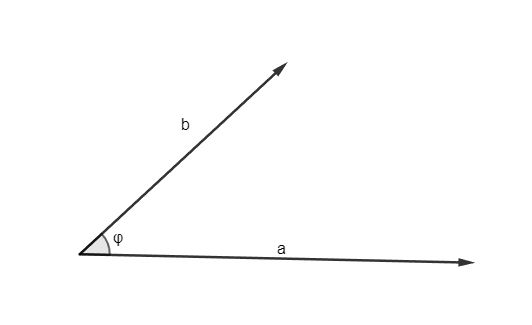
\includegraphics[height=7cm]{Images/Chapter_1/1-4-1.png}
\end{center}
Свойства: (\(\forall \vec a, \vec b \in V_3\))
\begin{enumerate}
    \item Симметричность: \(\vec a \cdot \vec b = \vec b \cdot \vec a\)

          Очевидно
    \item Аддитивность по 1-му аргументу: \(\forall \vec a_1, \vec a_2 \in V_3:
          (\vec a_1 + \vec a_2) \cdot \vec b = \vec a_1 \cdot \vec b + \vec a_2 \cdot \vec b\)

          \(\proj_{\vec b}\vec a\) --- Проекция \(\vec a\) на направление \(\vec b\).

          \(\proj_{\vec b}\vec a\ = |\vec a| \cos \varphi; \varphi = \angle(\vec a, \vec b) \in [0, \pi]\)

          \(\vec a = (a_x, a_y, a_z) \Rightarrow a_x = |\vec a| \cos\alpha;\; \alpha = \angle(\vec a, \vec i)\)
          \begin{center}
              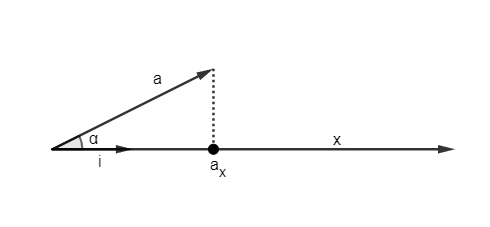
\includegraphics[height=7cm]{Images/Chapter_1/1-4-2.png}
          \end{center}
          \(a_x = \proj_{\vec i}\vec a = \vec i \cdot \vec a\),
          \(a_y = \proj_{\vec j}\vec a = \vec j \cdot \vec a\),
          \(a_z = \proj_{\vec k}\vec a = \vec k \cdot \vec a\)

          Выберем ДСК таким образом, что \(\vec i = \frac{\vec b}{|\vec b|}\) --- орт вектора \(\vec b\)
          \begin{center}
              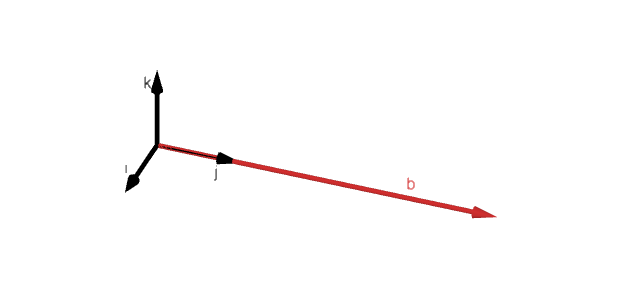
\includegraphics[height=7cm]{Images/Chapter_1/1-4-3.png}
          \end{center}
          \(\vec a = \vec a_1 + \vec a_2\)

          \((\vec a)_x = \proj_{\vec i}\vec a = \vec a \cdot \vec i =
          (\vec a_1 + \vec a_2) \cdot \frac{\vec b}{|\vec b|} =
          \frac{1}{|\vec b|} ((\vec a_1 + \vec a_2) \cdot \vec b)\)

          \(m = 1, 2: (\vec a_m)_x = \proj_{\vec i}\vec a_m = \vec a_m \cdot i =
          \vec a_m \cdot \frac{\vec b}{|\vec b|} =
          \frac{1}{|\vec b|} (\vec a_m \cdot \vec b)\)

          \(\begin{rcases*}
              \vec a = \frac{1}{|\vec b|} ((\vec a_1 + \vec a_2) \cdot \vec b) \\
              \vec a = \vec a_1 + \vec a_2 = \frac{1}{|\vec b|} (\vec a_1 \cdot \vec b) + \frac{1}{|\vec b|} (\vec a_2 \cdot \vec b)
          \end{rcases*} \Rightarrow \frac{1}{|\vec b|} ((\vec a_1 + \vec a_2) \cdot \vec b) =
          \frac{1}{|\vec b|} (\vec a_1 \cdot \vec b) + \frac{1}{|\vec b|} (\vec a_2 \cdot \vec b) \Rightarrow \\
          \Rightarrow (\vec a_1 + \vec a_2) \cdot \vec b = \vec a_1 \cdot \vec b + \vec a_2 \cdot \vec b \quad Q.E.D\)
    \item Однородность по 1-му аргументу: \(\forall \lambda \in \mathbb{R}: (\lambda \vec a)\cdot \vec b = \lambda(\vec a \cdot \vec b)\)
          \begin{center}
              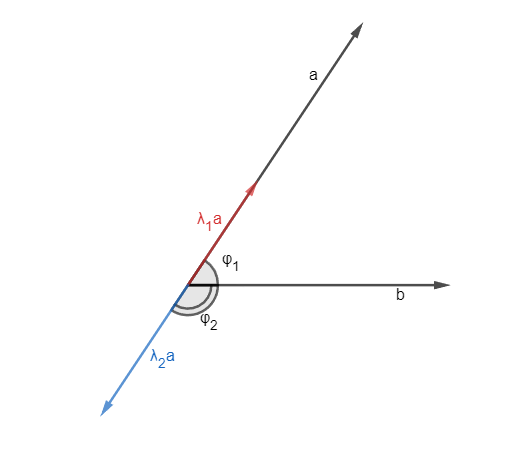
\includegraphics[height=7cm]{Images/Chapter_1/1-4-4.png}
          \end{center}
          \(|\lambda \vec a| = |\lambda| |\vec a|\)

          \(\lambda > 0: (\lambda \vec a)\cdot \vec b = |\lambda \vec a| |\vec b| \cos\varphi_1 = \lambda(|\vec a| |\vec b| \cos\varphi_1) = \lambda(\vec a \cdot \vec b)\)

          \(\lambda < 0: (\lambda \vec a)\cdot \vec b = |\lambda \vec a| |\vec b| \cos\varphi_2 = -\lambda(|\vec a| |\vec b| \cos\varphi_2) = \lambda(|\vec a| |\vec b| \cos(\pi - \varphi_2)) = \lambda(\vec a \cdot \vec b)\)

          \(\lambda = 0: (\lambda \vec a)\cdot \vec b = \vec 0 \cdot \vec b = 0 = 0(\vec a \cdot \vec b) = \lambda(\vec a \cdot \vec b)\)

          \(Q.E.D.\)
    \item \(\vec a \cdot \vec a \geq 0\). \(\vec a \cdot \vec a = 0 \Leftrightarrow \vec a = \vec 0\)

          Очевидно
\end{enumerate}
\(\begin{rcases*}
    2. \\
    3.
\end{rcases*} \Rightarrow\) Скалярное произведение линейно по 1-му аргументу.

\(\begin{rcases*}
    1. \\
    2. \\
    3.
\end{rcases*} \Rightarrow\) Скалярное произведение линейно по 2-му аргументу. \(\Rightarrow\)
Скалярное произведение линейно по всем своим аргументам.

Координатное представление:

\(\vec a = (a_1, a_2, a_3), \vec b = (b_1, b_2, b_3)\)

\(\vec a = a_1\vec i + a_2\vec j + a_3\vec k\)

\(\vec b = b_1\vec i + b_2\vec j + b_3\vec k\)

\(\vec a \cdot \vec b = (a_1\vec i + a_2\vec j + a_3\vec k) \cdot (b_1\vec i + b_2\vec j + b_3\vec k) = \text{(пользуясь 1. -- 4.)} = \\
= a_1 b_1 (\vec i \cdot \vec i) + a_1 b_2 (\vec i \cdot \vec j) + a_1 b_3 (\vec i \cdot \vec k) + \\
+ a_2 b_1 (\vec j \cdot \vec i) + a_2 b_2 (\vec j \cdot \vec j) + a_2 b_3 (\vec j \cdot \vec k) + \\
+ a_3 b_1 (\vec k \cdot \vec i) + a_3 b_2 (\vec k \cdot \vec j) + a_3 b_3 (\vec k \cdot \vec k) = \\
= \text{(все слагаемые кроме диагональных --- нули)} = \\
= a_1 b_1 (\vec i \cdot \vec i) + a_2 b_2 (\vec j \cdot \vec j) + a_3 b_3 (\vec k \cdot \vec k) = a_1 b_1 + a_2 b_2 + a_3 b_3\)


\subsection{Векторное произведение векторов}
\(``\times": V_3 \times V_3 \rightarrow V_3\)

\(\vec a, \vec b \in V_3 \rightarrow \vec c = [\vec a, \vec b] = \vec a \times \vec b \in V_3\)

\(\vec a \times \vec b = \vec c \defLeftrightarrow
\begin{cases}
    \vec c \perp \vec a, \vec b \text{ (плоскости, в которой лежат }\vec a, \vec b\text{)} \\
    \vec a, \vec b, \vec c \text{ --- правая тройка (определяется по правилу правой руки)} \\
    |\vec c| = |\vec a| |\vec b| \sin \varphi;\; \varphi = \angle(\vec a, \vec b)
\end{cases}\)
\begin{center}
    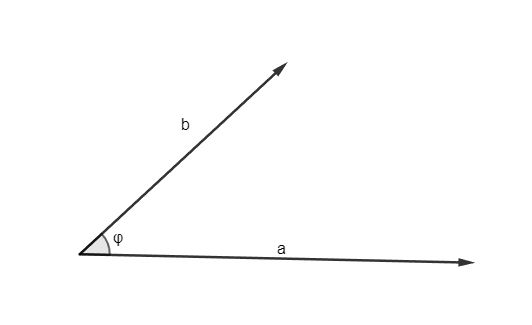
\includegraphics[height=7cm]{Images/Chapter_1/1-4-1.png}
\end{center}

\(\vec a \nparallel \vec b\). Если \(\vec a \parallel \vec b\), то \(\vec a \times \vec b = \vec 0\)

Свойства: (\(\forall \vec a, \vec b \in V_3\))
\begin{enumerate}
    \item Антисимметричность: \(\vec a \times \vec b = -\vec b \times \vec a\)

          Очевидно
    \item Аддитивность по 1-му аргументу: \(\forall \vec a_1, \vec a_2 \in V_3:
          (\vec a_1 + \vec a_2) \times \vec b = \vec a_1 \times \vec b + \vec a_2 \times \vec b\)

          Доказательство см. в 1.6
    \item Однородность по 1-му аргументу: \(\forall \lambda \in \mathbb{R}: (\lambda \vec a)\times \vec b = \lambda(\vec a \times \vec b)\)

          Очевидно
    \item \(|\vec a \times \vec b| = S(\text{параллелограмм, построенный на } \vec a, \vec b)\)

          Очевидно
\end{enumerate}

\(\begin{rcases*}
    2. \\
    3.
\end{rcases*} \Rightarrow\) Векторное произведение линейно по 1-му аргументу.

Координатное представление:

\(\vec a = (a_1, a_2, a_3) = a_1\vec i + a_2\vec j + a_3\vec k\)

\(\vec b = (b_1, b_2, b_3) = b_1\vec i + b_2\vec j + b_3\vec k\)

\(\vec c = (c_1, c_2, c_3) = c_1\vec i + c_2\vec j + c_3\vec k\)

\(\vec a \times \vec b = (a_1\vec i + a_2\vec j + a_3\vec k) \times (b_1\vec i + b_2\vec j + b_3\vec k) = \text{(пользуясь 1. -- 4.)} = \\
= a_1 b_1 (\vec i \times \vec i) + a_1 b_2 (\vec i \times \vec j) + a_1 b_3 (\vec i \times \vec k) + \\
+ a_2 b_1 (\vec j \times \vec i) + a_2 b_2 (\vec j \times \vec j) + a_2 b_3 (\vec j \times \vec k) + \\
+ a_3 b_1 (\vec k \times \vec i) + a_3 b_2 (\vec k \times \vec j) + a_3 b_3 (\vec k \times \vec k) = \\
= (\vec i \times \vec i = \vec j \times \vec j = \vec k \times \vec k = \vec 0; \\
\vec i \times \vec j = -(\vec j \times \vec i) = \vec k; \\
\vec k \times \vec i = -(\vec i \times \vec k) = \vec j; \\
\vec j \times \vec k = -(\vec k \times \vec j) = \vec i) = \\
= (a_2 b_3 - a_3 b_2)\vec i + (a_3 b_1 - a_1 b_3)\vec j + (a_1 b_2 - a_2 b_1)\vec k =
\begin{vmatrix}
    \vec i & \vec j & \vec k \\
    a_1    & a_2    & a_3    \\
    b_1    & b_2    & b_3
\end{vmatrix} = \vec i A_{11} + \vec j A_{12} + \vec k A_{13} = \\
= \left(
\begin{vmatrix}
        a_2 & a_3 \\
        b_2 & b_3
    \end{vmatrix}
, -
\begin{vmatrix}
        a_1 & a_3 \\
        b_1 & b_3
    \end{vmatrix}
,
\begin{vmatrix}
        a_1 & a_2 \\
        b_1 & b_2
    \end{vmatrix}
\right) =
(a_2 b_3 - a_3 b_2, a_3 b_1 - a_1 b_3, a_1 b_2 - a_2 b_1)\)


\subsection{Смешанное произведение векторов}
\(V_3 \times V_3 \times V_3 \rightarrow \mathbb{R}\)

Обозначения нет, вектора ставятся друг к другу без дополнительных знаков.

\(\vec a, \vec b, \vec c \in V_3 \rightarrow \vec a \vec b \vec c \in \mathbb{R}\)

\(\vec a \vec b \vec c \defeq (\vec a \times \vec b) \cdot \vec c\)

Свойства:
\begin{enumerate}
    \item \(|\vec a \vec b \vec c| = V(\text{параллелепипед, построенный на } \vec a, \vec b, \vec c)\),
          причём \(\vec a \vec b \vec c > 0 \Leftrightarrow \vec a, \vec b, \vec c\) --- правая тройка,
          \(\vec a \vec b \vec c < 0 \Leftrightarrow \vec a, \vec b, \vec c\) --- левая тройка.

          \begin{center}
              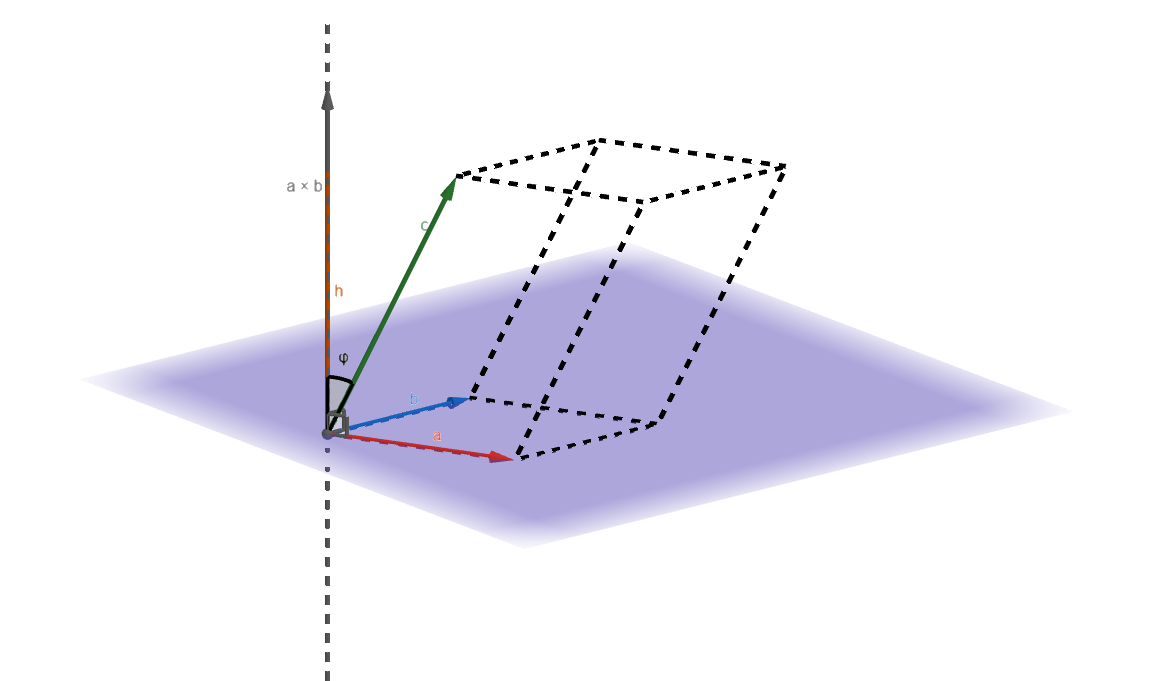
\includegraphics[height=7cm]{Images/Chapter_1/1-6-1.png}
          \end{center}

          \(\vec a \vec b \vec c = (\vec a \times \vec b) \cdot \vec c\),
          пусть \(\vec a \neq \vec 0\), \(\vec b \neq \vec 0\), \(\vec c \neq \vec 0\) (Если какой-либо вектор --- нулевой, то и произведение, и объём --- тоже нулевые)

          Пусть \(\vec a \nparallel \vec b\) (Иначе и произведение, и объём равны нулю)

          Построим \(\vec a \times \vec b\)
          \begin{itemize}
              \item \(\vec a, \vec b, \vec c\) --- правая тройка \(\Leftrightarrow \varphi = \angle(\vec a \times \vec b, \vec c) < 90^{\circ} \Leftrightarrow \cos\varphi > 0 \Leftrightarrow \vec a \vec b \vec c > 0\)
              \item \(\vec a, \vec b, \vec c\) --- левая тройка \(\Leftrightarrow \varphi = \angle(\vec a \times \vec b, \vec c) > 90^{\circ} \Leftrightarrow \cos\varphi < 0 \Leftrightarrow \vec a \vec b \vec c < 0\)
          \end{itemize}

          \(V := V(\text{параллелепипед, построенный на } \vec a, \vec b, \vec c) = \\
          = S(\text{параллелограмм, построенный на } \vec a, \vec b) \cdot h\), где \(h\) - высота параллелограмма.

          \(h = |\proj_{\vec a \times \vec b}\vec c| = ||\vec c| \cos \varphi|\)

          \(S(\text{параллелограмм, построенный на } \vec a, \vec b) = |\vec a \times \vec b|\)

          \(V = |\vec a \times \vec b| \cdot ||\vec c| \cos \varphi| = |(\vec a \times \vec b) \cdot \vec c| = |\vec a \vec b \vec c|\) \(Q.E.D.\)
    \item \(\vec a \vec b \vec c = \vec b \vec c \vec a = \vec c \vec a \vec b = -\vec c \vec b \vec a = -\vec b \vec a \vec c = -\vec a \vec c \vec b\)

          \(\vec a, \vec b, \vec c\) --- правая тройка \(\Leftrightarrow \vec a \vec b \vec c = V(\text{параллелепипед, построенный на } \vec a, \vec b, \vec c)\),
          а объём не зависит от того, какой вектор выбрать первым, значит:

          \(V = \vec a \vec b \vec c = \vec b \vec c \vec a = \vec c \vec a \vec b\)

          То же самое, если \(\vec a, \vec b, \vec c\) --- левая тройка, но со знаком минус.

    \item Аддитивность по первому (с 2., по любому) аргументу:
          \((\vec a_1 + \vec a_2)\vec b \vec c = \vec a_1 \vec b \vec c + \vec a_2 \vec b \vec c\)

          \((\vec a_1 + \vec a_2)\vec b \vec c = (\text{по 2.}) = \vec b \vec c (\vec a_1 + \vec a_2) =
          (\vec b \times \vec c) \cdot (\vec a_1 + \vec a_2) =
          (\vec b \times \vec c) \cdot \vec a_1 + (\vec b \times \vec c) \cdot \vec a_2 =
          \vec b \vec c \vec a_2 + \vec b \vec c \vec a_1 = (\text{по 2.}) =
          \vec a_1 \vec b \vec c + \vec a_2 \vec b \vec c\) \(Q.E.D.\)
    \item Однородность по первому (с 2., по любому) аргументу:
          \((\lambda\vec a)\vec b \vec c = \lambda(\vec a \vec b \vec c)\)

          \((\lambda\vec a)\vec b \vec c = (\text{по 2.}) = \vec b \vec c (\lambda\vec a) =
          (\vec b \times \vec c) \cdot (\lambda\vec a) =
          \lambda((\vec b \times \vec c) \cdot \vec a) =
          \lambda(\vec b \vec c \vec a) = (\text{по 2.}) =
          \lambda(\vec a \vec b \vec c)\) \(Q.E.D.\)
\end{enumerate}

Координатное представление:

\(\vec a \vec b \vec c = (\vec a \times \vec b) \cdot \vec c =
\begin{vmatrix}
    \vec i & \vec j & \vec k \\
    a_1    & a_2    & a_3    \\
    b_1    & b_2    & b_3
\end{vmatrix} \cdot \vec c =
\begin{vmatrix}
    c_1 & c_2 & c_3 \\
    a_1 & a_2 & a_3 \\
    b_1 & b_2 & b_3
\end{vmatrix} =
\begin{vmatrix}
    a_1 & a_2 & a_3 \\
    b_1 & b_2 & b_3 \\
    c_1 & c_2 & c_3
\end{vmatrix}\)

Доказательство аддитивности векторного произведения:

\(\forall \vec a_1, \vec a_2, \vec b \in V_3\)

\((\vec a_1 + \vec a_2)\vec b \vec c = ((\vec a_1 + \vec a_2) \times \vec b) \cdot \vec c = \vec a_1 \vec b \vec c + \vec a_2 \vec b \vec c\)

Пусть \(\vec c = \vec i\). Тогда: \((\vec a_1 + \vec a_2)\vec b \vec c = ((\vec a_1 + \vec a_2) \times \vec b) \cdot \vec i = ((\vec a_1 + \vec a_2) \times \vec b)_x\)

\(m = 1, 2:\; (\vec a_m \times \vec b) \cdot \vec c = (\vec a_m \times \vec b) \cdot \vec i = (\vec a_m \times \vec b)_x\)

\((\vec a_1 + \vec a_2)\vec b \vec c = \vec a_1 \vec b \vec c + \vec a_2 \vec b \vec c \Leftrightarrow ((\vec a_1 + \vec a_2) \times \vec b)_x = (\vec a_1 \times \vec b)_x + (\vec a_2 \times \vec b)_x\)

Повторим то же самое, но с \(\vec c = \vec j\) и \(\vec c = \vec k\).

\(\begin{rcases}
    ((\vec a_1 + \vec a_2) \times \vec b)_x = (\vec a_1 \times \vec b)_x + (\vec a_2 \times \vec b)_x \\
    ((\vec a_1 + \vec a_2) \times \vec b)_y = (\vec a_1 \times \vec b)_y + (\vec a_2 \times \vec b)_y \\
    ((\vec a_1 + \vec a_2) \times \vec b)_z = (\vec a_1 \times \vec b)_z + (\vec a_2 \times \vec b)_z
\end{rcases} \Leftrightarrow (\vec a_1 + \vec a_2) \times \vec b = (\vec a_1 \times \vec b) + (\vec a_2 \times \vec b)\) \(Q.E.D.\)

Двойное векторное произведение

\(\vec a \times (\vec b \times \vec c) = \vec b(\vec a \cdot \vec c) - \vec c(\vec a \cdot \vec b)\)
\begin{itemize}
    \item \(\vec b \nparallel \vec c\):
          \begin{center}
              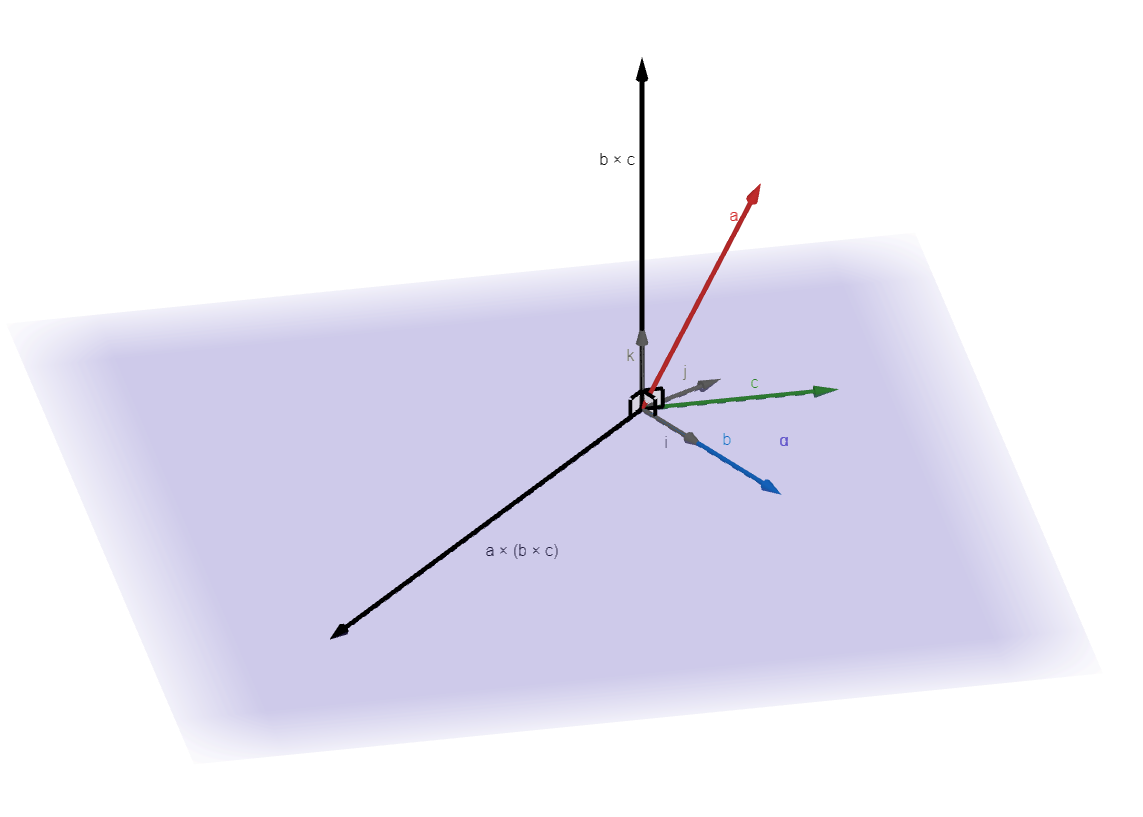
\includegraphics[height=7cm]{Images/Chapter_1/1-7-1.png}
          \end{center}
          Проведём плоскость \(\alpha(\vec b, \vec c) \Rightarrow \vec b \times \vec c \perp \alpha\)

          \(\vec a \times (\vec b \times \vec c) \perp \vec b \times \vec c \Rightarrow \vec a \times (\vec b \times \vec c) \in \alpha\)

          Введём ДСК, где \(\vec i = \frac{\vec b}{|\vec b|}\), \(\vec j \in \alpha\), \(\vec k \perp \alpha\). Тогда:

          \(\vec b = (b_1, 0, 0);\; \vec c = (c_1, c_2, 0);\; \vec a = (a_1, a_2, a_3)\)

          \(\vec b \times \vec c = (b_1, 0, 0) \times (c_1, c_2, 0) = (0, 0, b_1 c_2)\)

          \(\vec a \times (\vec b \times \vec c) = (a_1, a_2, a_3) \times (0, 0, b_1 c_2) = (a_2 b_1 c_2, -a_1 b_1 c_2, 0)\)

          \(\vec b(\vec a \cdot \vec c) - \vec c(\vec a \cdot \vec b) = \vec b a_1 c_1 + \vec b a_2 c_2 - \vec c a_1 b_1 =
          (b_1(a_1 c_1 + a_2 c_2) - c_1 a_1 b_1, -c_2 a_1 b_1, 0) =
          (a_2 b_1 c_2, -a_1 b_1 c_2, 0) = \vec a \times (\vec b \times \vec c)\) \(Q.E.D.\)
    \item \(\vec b \parallel \vec c\):

          \(\vec b \times \vec c = \vec 0\)

          \(\exists \lambda \in \mathbb{R}: \vec b = \lambda \vec c\)

          \(\begin{rcases}
              \vec b(\vec a \cdot \vec c) = \lambda c(\vec a \cdot \vec c) \\
              \vec c(\vec a \cdot \vec b) = \vec c(\vec a \cdot \lambda\vec c) = \lambda \vec c(\vec a \cdot \vec c)
          \end{rcases} \Rightarrow \vec b(\vec a \cdot \vec c) - \vec c(\vec a \cdot \vec b) = \vec 0 = \vec b \times \vec c\) \(Q.E.D.\)
\end{itemize}


\section{Прямая на плоскости, плоскость и прямая в пространстве}
\subsection{Линейное уравнение}

На плоскости (в пространстве) в ДСК \(Oxy\) (\(Oxyz\)) уравнение \(Ax + By + C = 0\), \(A^2 + B^2 \neq 0\) (\(Ax + By + Cz + D = 0\), \(A^2 + B^2 + C^2 \neq 0\)) --- алгебраическое уравнение первого порядка или линейное уравнение.

Любое линейное уравнение на плоскости (в пространстве) определяет прямую (плоскость), и наоборот, любая прямая (плоскость) на плоскости (в пространстве) может быть описана линейным уравнением.

Доказывать будем для прямой в плоскости. Доказательство для прямой в пространстве полностью аналогично.
\begin{enumerate}
    \item Уравнение \(\rightarrow\) прямая:
          \begin{center}
              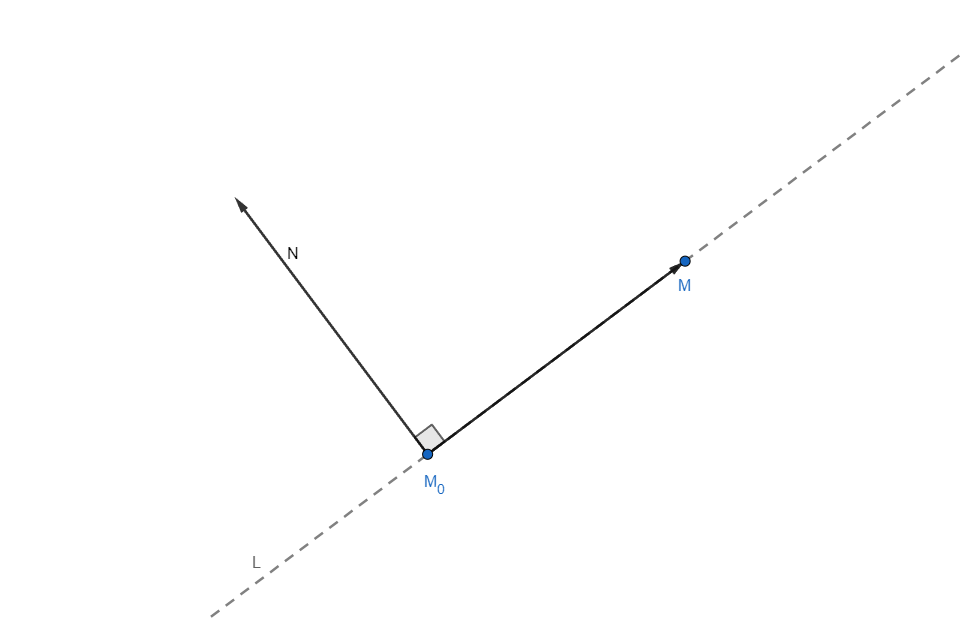
\includegraphics[height=7cm]{Images/Chapter_1/2-1-1.png}
          \end{center}
          \(Ax + By + C = 0\), \(A^2 + B^2 \neq 0\)
          Не умаляя общности, пусть \(B \neq 0\). Тогда \(M_0(x_0, y_0) = (0, \frac{-C}{B})\) - удовлетворяет уравнению.

          Пусть \(M(x, y) \neq M\) - тоже удовлетворяет уравнению. Тогда \(A(x - x_0) + B(y - y_0) = 0\).

          \(\overrightarrow{M_0 M} = (x - x_0, y - y_0)\)

          \(\vec N := (A, B) \neq 0\)

          \(M_0(x_0, y_0) = (0, \frac{-C}{B}) \Leftrightarrow \overrightarrow{M_0 M} \cdot \vec N = 0 \Leftrightarrow \vec N \perp \overrightarrow{M_0 M} \Rightarrow \\
          \Rightarrow \forall M(x, y) \text{, удовлетворяющих } A(x - x_0) + B(y - y_0) = 0: M \in L \perp \vec N, M_0 \in L\)

          И наоборот, если \(M \in L\), то \(\overrightarrow{M_0 M} \perp \vec N \Rightarrow M \text{ удовлетворяет } A(x - x_0) + B(y - y_0) = 0\)

          \(Ax + By + C = 0\) Определяет прямую \(L\) и никакую другую, т.к. Если \(M \notin L\), то \(\overrightarrow{M_0 M} \not\perp \vec N \Rightarrow M \text{ не удовлетворяет } A(x - x_0) + B(y - y_0) = 0\) \(Q.E.D.\)
    \item Прямая \(\rightarrow\) уравнение:
          \begin{center}
              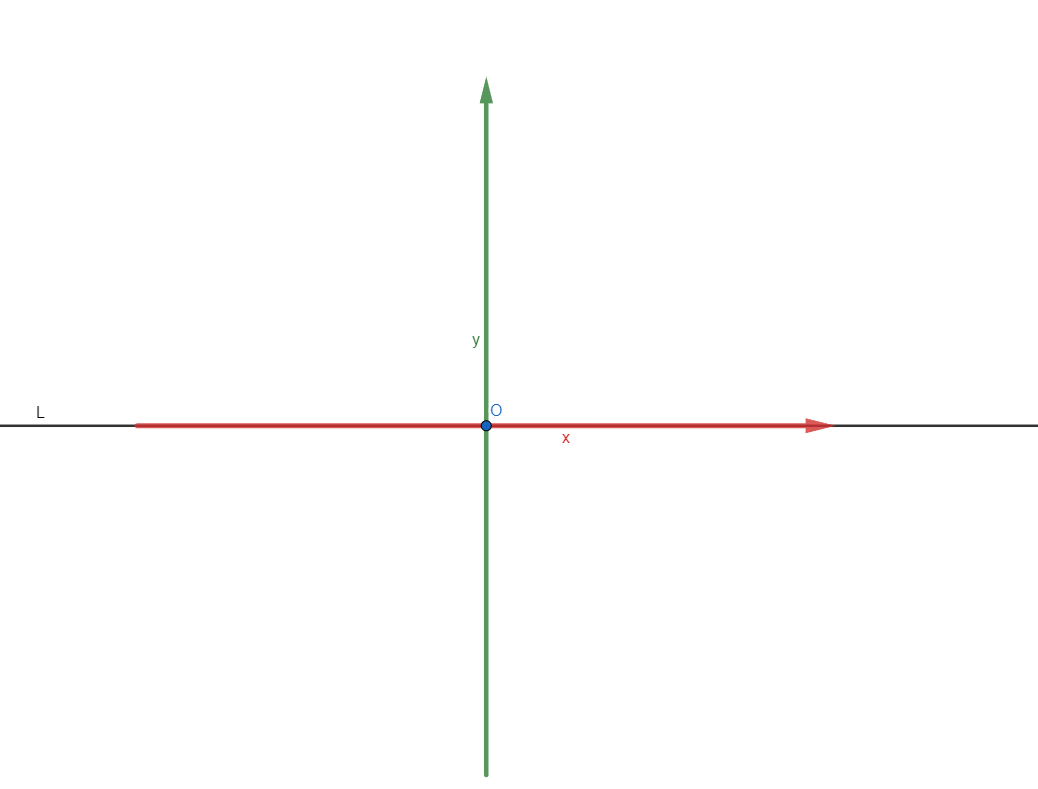
\includegraphics[height=7cm]{Images/Chapter_1/2-1-2.png}
          \end{center}
          Пусть \(L\) --- прямая на плоскости.

          Введём ДСК так, чтобы \(L\) совпадала с \(Ox\). Тогда очевидно, что линейное уравнение \(y = 0\) содержит все точки \(L\).

          Если есть ДСК, в которой \(L\) задаётся линейным уравнением, то в любой другой ДСК \(L\) будет задаваться линейным уравнением.
          Любые две ДСК связаны поворотом и сдвигом, значит нужно доказать, что при повороте и сдвиге линейное уравнение остаётся линейным уравнением.

          \begin{itemize}
              \item Сдвиг:
                    \begin{center}
                        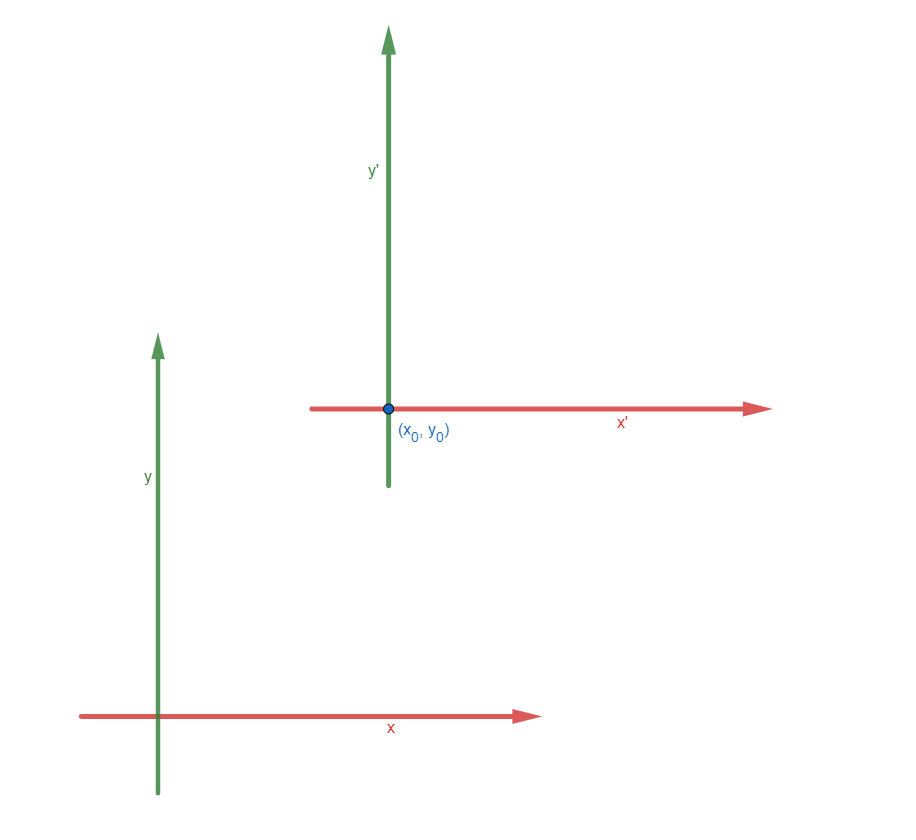
\includegraphics[height=7cm]{Images/Chapter_1/2-1-3.png}
                    \end{center}
                    \(x = x' + x_0\)

                    \(y = y' + y_0\)

                    \(A(x' + x_0) + B(y' + y_0) + C = 0 \Rightarrow Ax' + By' + (Ax_0 + By_0 + C) = 0\)

                    \(C' := (Ax_0 + By_0 + C)\)

                    \(Ax + By + C' = 0\) - тоже линейное уравнение.
              \item Поворот:
                    \begin{center}
                        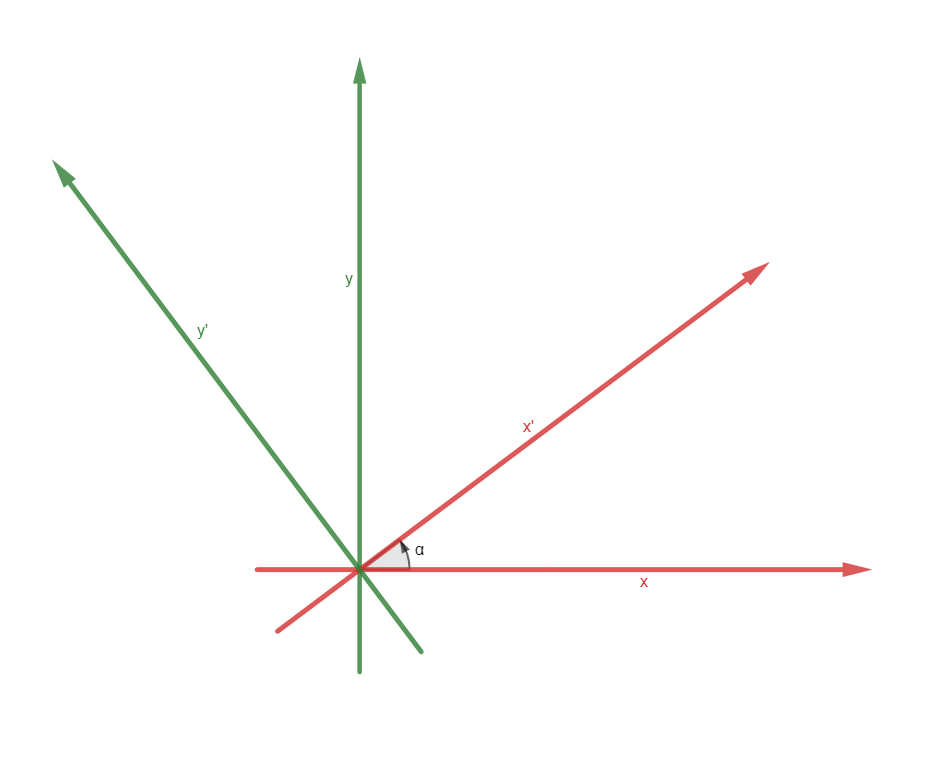
\includegraphics[height=7cm]{Images/Chapter_1/2-1-4.png}
                    \end{center}
                    \(x = x'\cos\alpha - y'\sin\alpha\)

                    \(y = x'\sin\alpha + y'\cos\alpha\)

                    \(A(x'\cos\alpha - y'\sin\alpha) + B(x'\sin\alpha + y'\cos\alpha) + C = 0 \Rightarrow (A\cos\alpha + B\sin\alpha)x' + (B\cos\alpha - A\sin\alpha)y' + C = 0\)

                    \(A' := A\cos\alpha + B\sin\alpha\)

                    \(B' := B\cos\alpha - A\sin\alpha\)

                    \(A'^2 + B'^2 = A^2 + B^2 \neq 0\), значит \(A'x + B'y + C = 0\) - тоже линейное уравнение.
          \end{itemize}
          Значит если прямая задаётся линейным уравнением в ДСК, то в любой другой ДСК эта прямая будет задаваться линейным уравнением \(\quad Q.E.D.\)
\end{enumerate}

\(Ax + By + C = 0\), \(A^2 + B^2 \neq 0\) --- Общее уравнение прямой на плоскости, \(\vec N = (A, B)\) --- Вектор нормали.

\(Ax + By + Cz + D = 0\), \(A^2 + B^2 + C^2\neq 0\) --- Общее уравнение плоскости в пространстве, \(\vec N = (A, B, C)\) --- Вектор нормали.

\subsection{Способы задания}
\begin{center}
    \begin{longtable}[t]{|p{5.5cm}|p{5.5cm}|p{5.5cm}|}
        \hline
        Прямая в плоскости
         &
        Плоскость в пространстве
         &
        Прямая в пространстве
        \\
        \hline
        Общее уравнение:
        \begin{center}
            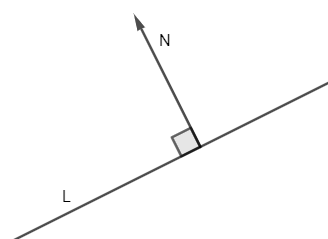
\includegraphics[width=5.5cm]{Images/Chapter_1/2-2-1.png}
        \end{center}
        \fbox{\(Ax + By + C = 0\)}

        \(A^2 + B^2 \neq 0\)

        \(\vec N = (A, B)\) --- нормаль. \(\vec N \perp L\).

        \(C = 0 \Rightarrow L \cap (0, 0)\)
         &
        Общее уравнение:
        \begin{center}
            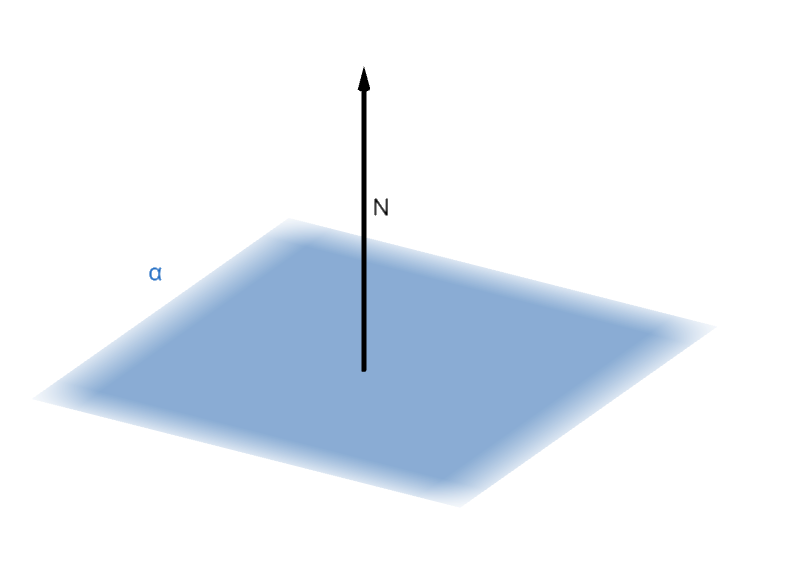
\includegraphics[width=5.5cm]{Images/Chapter_1/2-2-10.png}
        \end{center}
        \fbox{\(Ax + By + Cz + D = 0\)}

        \(A^2 + B^2 + C^2 \neq 0\)

        \(\vec N = (A, B, C)\) --- нормаль. \(\vec N \perp \alpha\).

        \(C = 0 \Rightarrow \alpha \cap (0, 0, 0)\)
         &
        Пересечение плоскостей:
        \begin{center}
            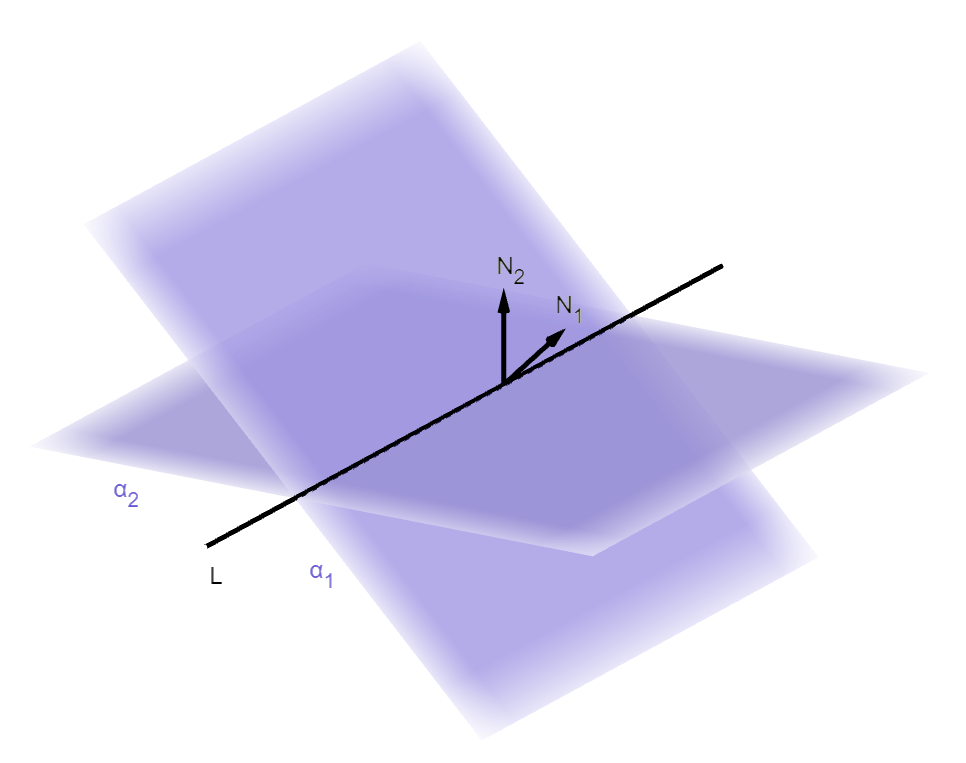
\includegraphics[width=5.5cm]{Images/Chapter_1/2-2-18.png}
        \end{center}
        \(L = \alpha_1 \cap \alpha_2\)

        \scriptsize\fbox{\(L:
            \begin{cases}
                A_1 x + B_1 y + C_1 z + D_1 = 0 \\
                A_2 x + B_2 y + C_2 z + D_2 = 0
            \end{cases}\)}\normalsize

        \(A_i^2 + B_i^2 + C_i^2 \neq 0\)

        \(\vec N_1 \nparallel \vec N_2\)
        \\
        \hline
        Уравнение в отрезках:
        \begin{center}
            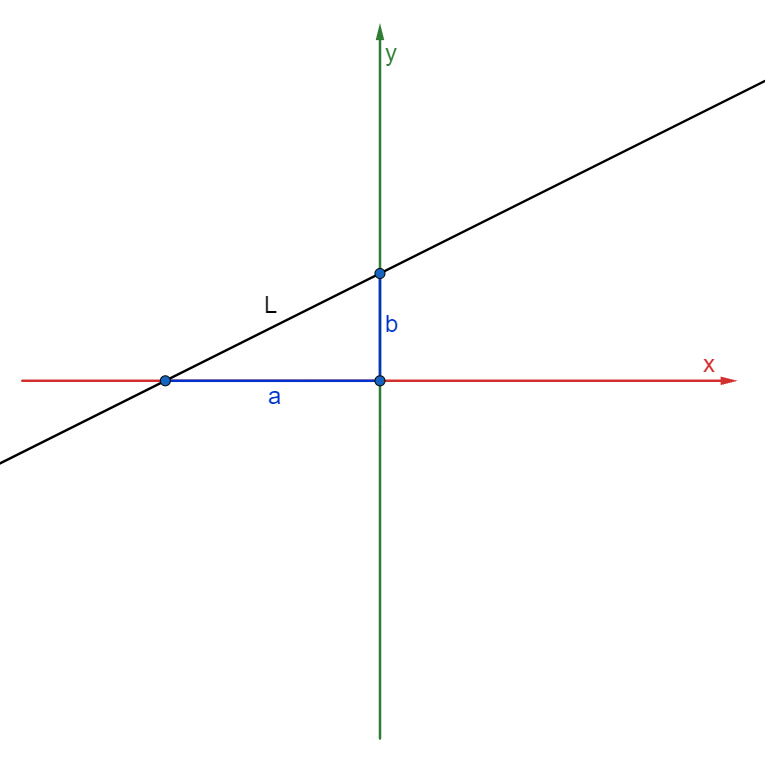
\includegraphics[width=5.5cm]{Images/Chapter_1/2-2-2.png}
        \end{center}
        \((0, 0) \notin L\)

        \fbox{\(\dfrac{x}{a} + \dfrac{y}{b} = 1\)}

        \(a^2 + b^2 \neq 0\)
         &
        Уравнение в отрезках:
        \begin{center}
            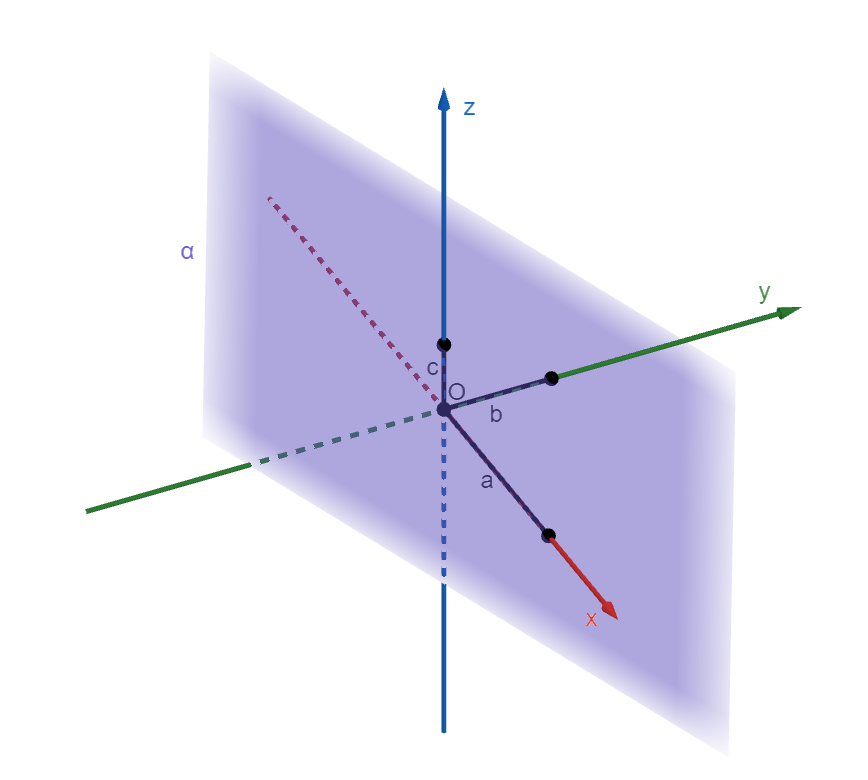
\includegraphics[width=5.5cm]{Images/Chapter_1/2-2-11.png}
        \end{center}
        \((0, 0, 0) \notin \alpha\)

        \fbox{\(\dfrac{x}{a} + \dfrac{y}{b} + \dfrac{z}{c} = 1\)}

        \(a^2 + b^2 + c^2 \neq 0\)
         &
        Пересечение плоскостей \(\rightarrow\) каноническое уравнение:
        \begin{center}
            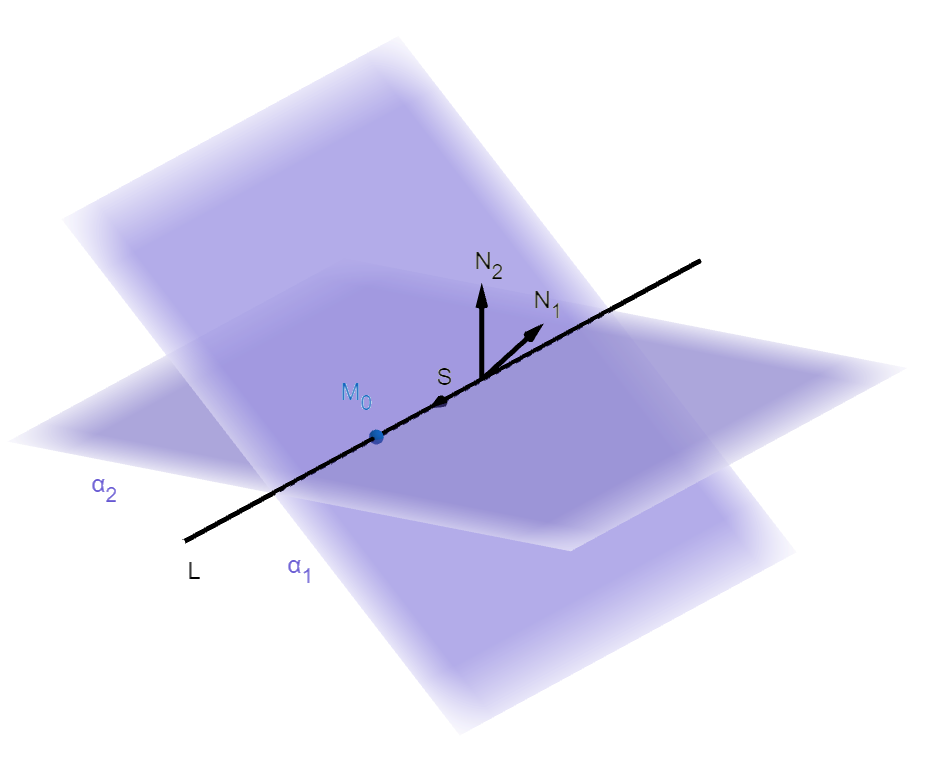
\includegraphics[width=5.5cm]{Images/Chapter_1/2-2-19.png}
        \end{center}
        \(\vec S \perp \vec N_1, \vec S \perp \vec N_2\)

        \(\vec S = \vec N_1 \times \vec N_2\)

        Пусть \(M_0 = (x_0, y_0, 0) = L \cap Oz\)

        Тогда решим систему:

        \small\fbox{\(L:
            \begin{cases}
                A_1 x_0 + B_1 y_0 + D_1 = 0 \\
                A_2 x_0 + B_2 y_0 + D_2 = 0
            \end{cases}\)}\normalsize

        Если не получилось, то \(M_0 = (x_0, 0, z_0) = L \cap Oy\)

        Cнова не получилось: \(M_0 = (0, y_0, z_0) = L \cap Ox\)
        \\
        \hline
        Уравнение через нормаль и точку:
        \begin{center}
            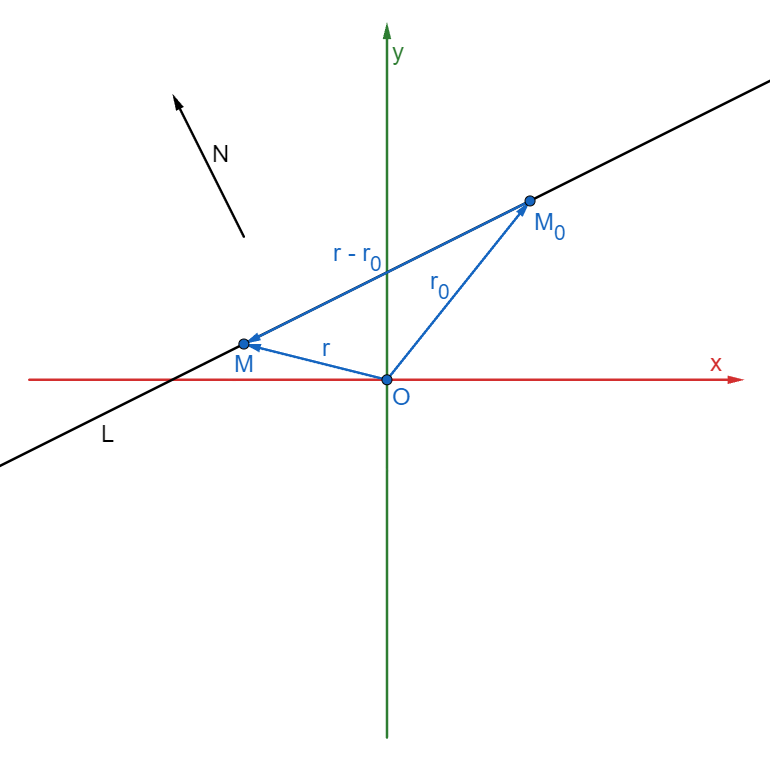
\includegraphics[width=5.5cm]{Images/Chapter_1/2-2-3.png}
        \end{center}
        \(M_0(x_0, y_0) \in L\)

        \(\vec N(A, B) \perp L\)

        \(M(x, y) \in L\)

        \(\vec r_0 = \overrightarrow{OM_0} = (x_0, y_0)\)

        \(\vec r = \overrightarrow{OM} = (x, y)\)

        \(\overrightarrow{M_0M} = \vec r - \vec r_0 \perp \vec N \Leftrightarrow\)

        \(\Leftrightarrow\) \fbox{\((\vec r - \vec r_0) \cdot \vec N = 0\)} \(\Leftrightarrow\)

        \small\(\Leftrightarrow\)\fbox{\(A(x - x_0) + B(y - y_0) = 0\)}\normalsize

        \(\)
         &
        Уравнение через нормаль и точку:
        \begin{center}
            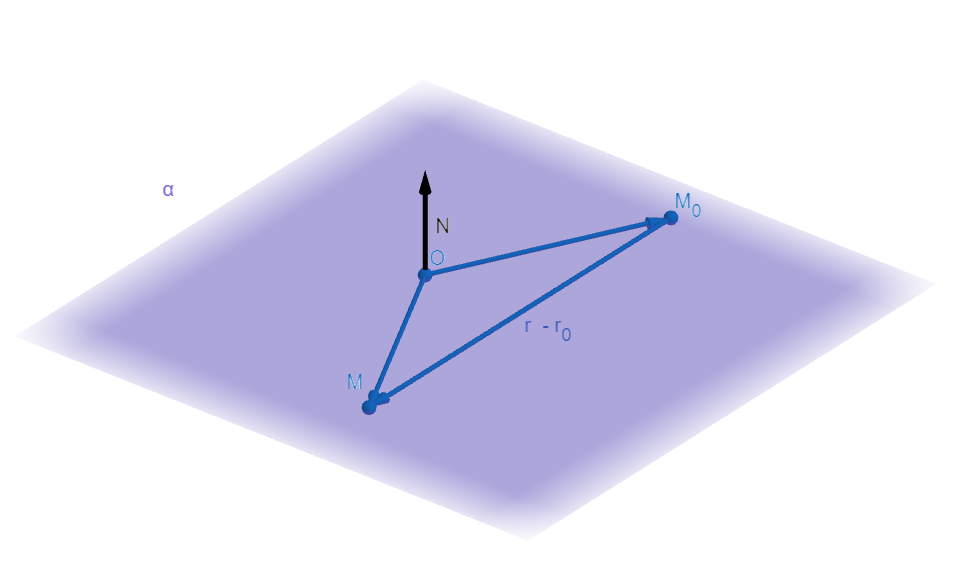
\includegraphics[width=5.5cm]{Images/Chapter_1/2-2-12.png}
        \end{center}
        \(M_0(x_0, y_0, z_0) \in \alpha\)

        \(\vec N(A, B, C) \perp \alpha\)

        \(M(x, y, z) \in \alpha\)

        \(\vec r_0 = \overrightarrow{OM_0} = (x_0, y_0, z_0)\)

        \(\vec r = \overrightarrow{OM} = (x, y, z)\)

        \(\overrightarrow{M_0M} = \vec r - \vec r_0 \perp \vec N \Leftrightarrow\)

        \(\Leftrightarrow\) \fbox{\((\vec r - \vec r_0) \cdot \vec N = 0\)}\(\Leftrightarrow\)

        \scriptsize\(\Leftrightarrow\)\fbox{\(A(x - x_0) + B(y - y_0) + C(z - z_0) = 0\)}\normalsize

        \(\)
         &
        Каноническое уравнение \(\rightarrow\) пересечение плоскостей:

        \scriptsize\(L:
        \begin{cases}
            l(x - x_0) + m(y - y_0) = 0 \\
            l(x - x_0) + n(z - z_0) = 0
        \end{cases}\)\normalsize

        Где \((l, m, n) = \vec S\) - направляющий вектор прямой \(L\),

        \((x_0, y_0, z_0) = M_0 \in L\)
        \\
        \hline
        Каноническое / параметрическое уравнение:
        \begin{center}
            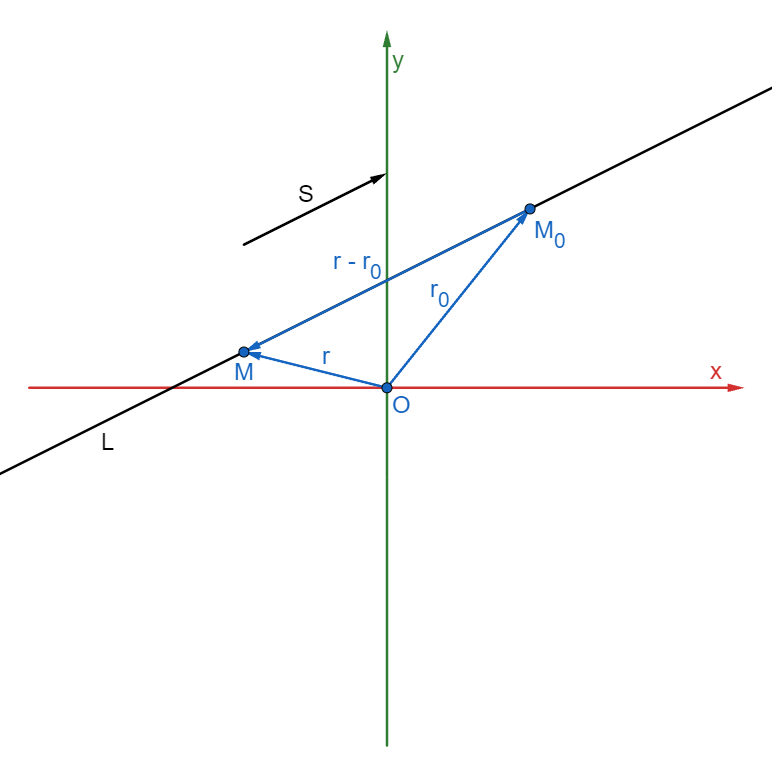
\includegraphics[width=5.5cm]{Images/Chapter_1/2-2-4.png}
        \end{center}
        \(M_0(x_0, y_0) \in L\)

        \(\vec S(l, m) \parallel L\)

        \(M(x, y) \in L\)

        \(\vec r_0 = \overrightarrow{OM_0} = (x_0, y_0)\)

        \(\vec r = \overrightarrow{OM} = (x, y)\)

        \(\overrightarrow{M_0M} = \vec r - \vec r_0 \parallel \vec S \Leftrightarrow\)

        \(\Leftrightarrow \exists t \in \mathbb{R}: \vec r - \vec r_0 = t \vec S \Leftrightarrow\)

        \(\Leftrightarrow\)\fbox{\(\dfrac{x - x_0}{l} = \dfrac{y - y_0}{m} = t\)}

        \fbox{\(\vec r = \vec r_0 + t \vec S\)}

        \fbox{
            \(
            \begin{cases}
                x = x_0 + tl \\
                y = y_0 + tm
            \end{cases}
            \)
        }

        \(\)
         &
        Условие принадлежности четырёх точек плоскости:
        \begin{center}
            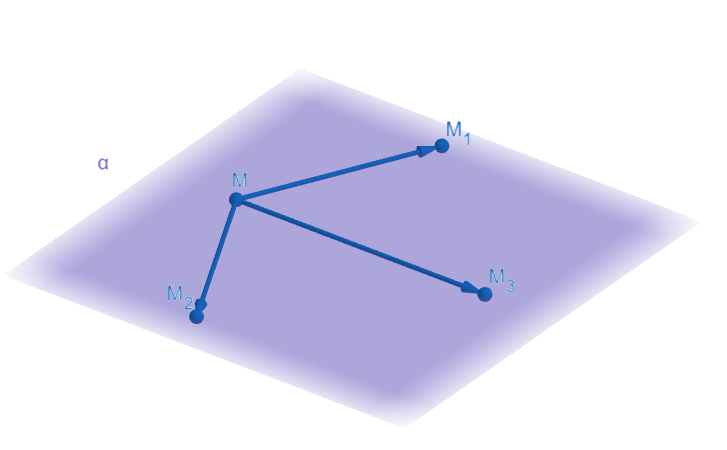
\includegraphics[width=5.5cm]{Images/Chapter_1/2-2-13.png}
        \end{center}
        \(M, M_1, M_2, M_3 \in \alpha\):

        \fbox{\(\overrightarrow{MM_1}\overrightarrow{MM_2}\overrightarrow{MM_3} = 0\)}
         &
        Каноническое / параметрическое уравнение:
        \begin{center}
            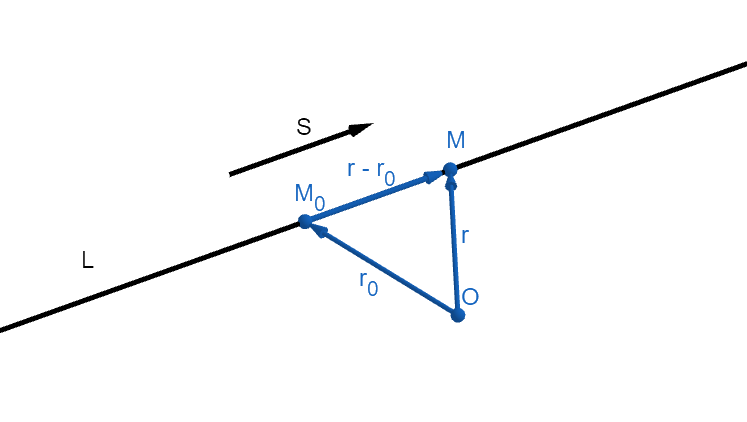
\includegraphics[width=5.5cm]{Images/Chapter_1/2-2-20.png}
        \end{center}
        \(M_0(x_0, y_0, z_0) \in L\)

        \(\vec S(l, m, n) \parallel L\)

        \(M(x, y, z) \in L\)

        \(\vec r_0 = \overrightarrow{OM_0} = (x_0, y_0, z_0)\)

        \(\vec r = \overrightarrow{OM} = (x, y, z)\)

        \(\overrightarrow{M_0M} = \vec r - \vec r_0 \parallel \vec S \Leftrightarrow\)

        \scriptsize\(\Leftrightarrow\)\fbox{\(\dfrac{x - x_0}{l} = \dfrac{y - y_0}{m} = \dfrac{z - z_0}{n} = t\)}\normalsize

        \fbox{\(\vec r = \vec r_0 + t \vec S\)}

        \fbox{
            \(
            \begin{cases}
                x = x_0 + tl \\
                y = y_0 + tm \\
                z = z_0 + tn
            \end{cases}
            \)
        }

        \(\)
        \\
        \hline
        Нормальное уравнение:
        \begin{center}
            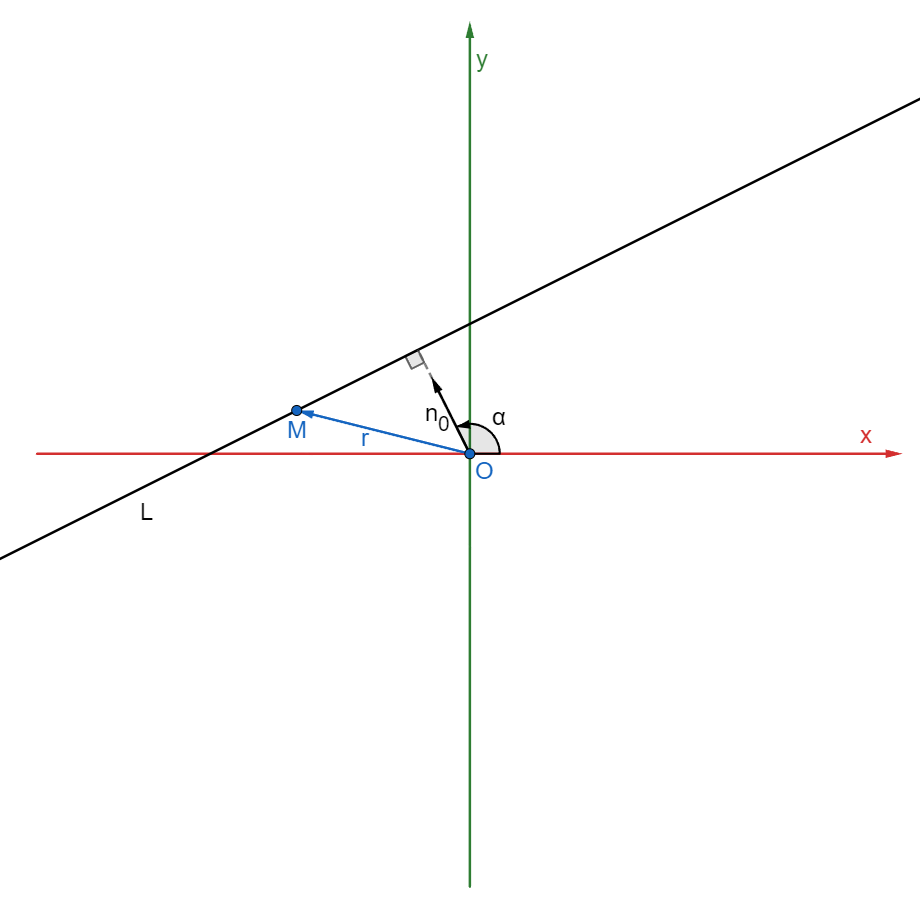
\includegraphics[width=5.5cm]{Images/Chapter_1/2-2-5.png}
        \end{center}
        \(O(0, 0) \notin L\)

        \(P = |O, L| > 0\)

        \(\vec n_0 \perp L\), \(|\vec n_0| = 1\)

        \(\vec n_0\) направлен в сторону \(L\) если его приложить к \(O\)

        \(\vec n_0 = (\cos \alpha, \sin \alpha)\)

        \(M(x, y) \in L\)

        \(P = \proj_{\vec n_0} \vec r \Leftrightarrow\)

        \(\Leftrightarrow\) \fbox{\(\vec r \cdot \vec n_0 - P = 0\)}

        \fbox{\(x \cos \alpha + y \sin \alpha - P = 0\)}

        \(L: Ax + By + C = 0\), \(A^2 + B^2 \neq 0\)

        \(\vec N = (A, B) \perp L \Rightarrow\)

        \(\Rightarrow \vec n_0 = \dfrac{\pm \vec N}{|\vec N|} = \)

        \small\(= \pm \left(\dfrac{A}{\sqrt{A^2 + B^2}}, \dfrac{B}{\sqrt{A^2 + B^2}}\right)\)\normalsize

        \(C > 0: ``+"\)

        \(C < 0: ``-"\)

        \(\cos \alpha = \dfrac{\pm A}{\sqrt{A^2 + B^2}}\)

        \(\sin \alpha = \dfrac{\pm B}{\sqrt{A^2 + B^2}}\)

        \(P = \dfrac{\pm C}{\sqrt{A^2 + B^2}}\)
         &
        Нормальное уравнение:
        \begin{center}
            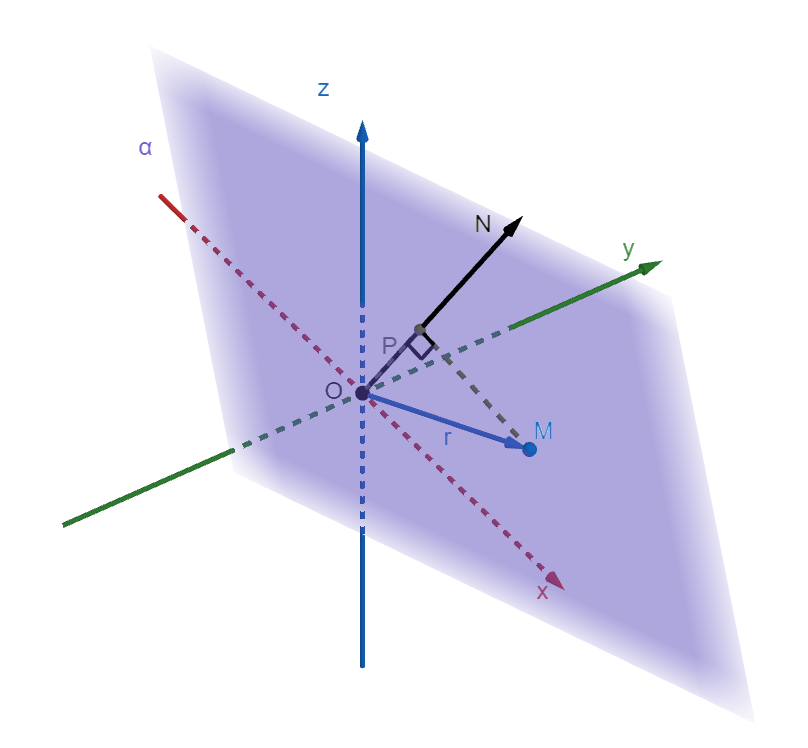
\includegraphics[width=5.5cm]{Images/Chapter_1/2-2-14.png}
        \end{center}
        \(O(0, 0, 0) \notin L\)

        \(P = |O, \alpha| > 0\)

        \(\vec n_0 \perp \alpha\), \(|\vec n_0| = 1\)

        \(\vec n_0\) направлен в сторону \(\alpha\) если его приложить к \(O\)

        \(\vec n_0 = (\cos \alpha, \cos \beta, \cos \gamma)\)

        \(M(x, y, z) \in \alpha\)

        \(P = \proj_{\vec n_0} \vec r \Leftrightarrow\)

        \(\Leftrightarrow\) \fbox{\(\vec r \cdot \vec n_0 - P = 0\)}

        \scriptsize\fbox{\(x \cos \alpha + y \cos \beta + z \cos \gamma - P = 0\)}\normalsize

        \(\alpha: Ax + By + Cz + D = 0\), \(A^2 + B^2 + C^2 \neq 0\)

        \(\vec N = (A, B, C) \perp L \Rightarrow\)

        \(\Rightarrow \vec n_0 = \dfrac{\pm \vec N}{|\vec N|}\)

        \(C > 0: ``+"\)

        \(C < 0: ``-"\)

        \(\cos \alpha = \dfrac{\pm A}{\sqrt{A^2 + B^2 + C^2}}\)

        \(\cos \beta = \dfrac{\pm B}{\sqrt{A^2 + B^2 + C^2}}\)

        \(\cos \gamma = \dfrac{\pm C}{\sqrt{A^2 + B^2 + C^2}}\)

        \(P = \dfrac{\pm D}{\sqrt{A^2 + B^2 + C^2}}\)
         &

        \\
        \hline
        Расстояние от точки до прямой:
        \begin{center}
            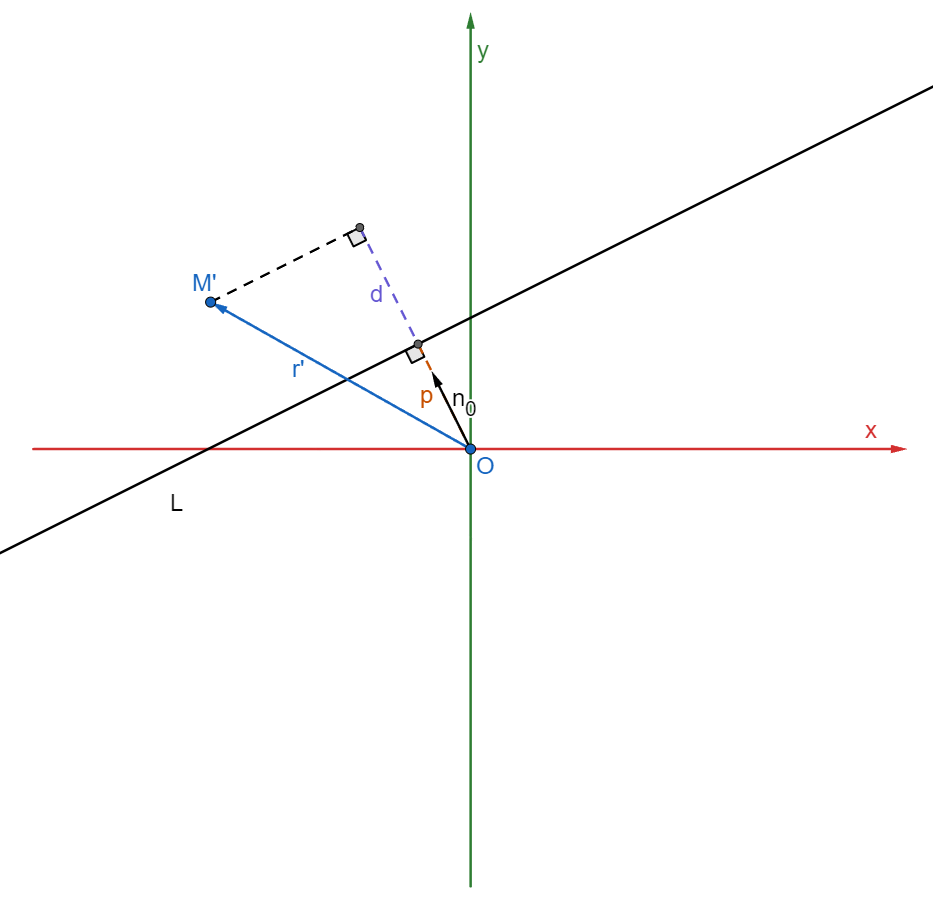
\includegraphics[width=5.5cm]{Images/Chapter_1/2-2-6.png}
        \end{center}
        \(M(x', y')\)

        \(\vec{r'} = \overrightarrow{OM'} = (x', y')\)

        \(L\) задана нормальным уравнением

        \(\proj_{\vec n_0} \vec{r'} - P = \delta\) --- отклонение

        \(\delta > 0\), если \(M'\) и \(O\) лежат по разные стороны от \(L\)

        \(\delta < 0\), если \(M'\) и \(O\) лежат по одну сторону от \(L\)

        \(d = |M', L| = |\delta| = \)

        \(=\) \fbox{\(|\vec{r'} \cdot \vec n_0 - P|\)} \(=\)

        \small\(=\) \fbox{\(|x' \cos \alpha + y' \sin \alpha - P|\)} \(=\)\normalsize

        \(L: Ax + By + C = 0\)

        \fbox{\(d = \dfrac{|Ax' + By' + C|}{\sqrt{A^2 + B^2}}\)}

        \small Работает даже если \(O \in L\)\normalsize
         &
        Расстояние от точки до плоскости:
        \begin{center}
            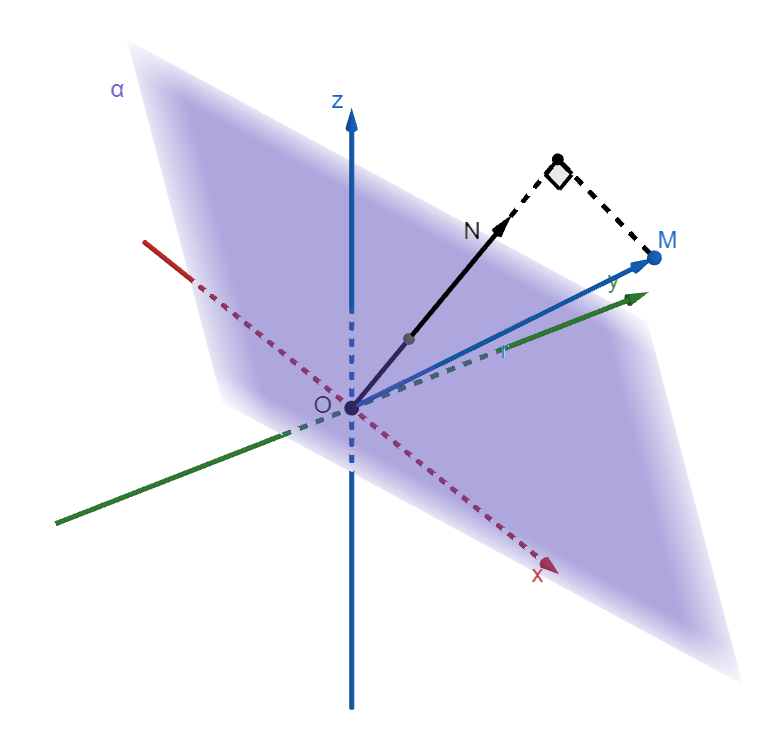
\includegraphics[width=5.5cm]{Images/Chapter_1/2-2-15.png}
        \end{center}
        \(M(x', y', z')\)

        \(\vec{r'} = \overrightarrow{OM'} = (x', y', z')\)

        \(\alpha\) задана нормальным уравнением

        \(\proj_{\vec n_0} \vec{r'} - P = \delta\) --- отклонение

        \(\delta > 0\), если \(M'\) и \(O\) лежат по разные стороны от \(\alpha\)

        \(\delta < 0\), если \(M'\) и \(O\) лежат по одну сторону от \(\alpha\)

        \(d = |M', \alpha| = |\delta| = \)

        \(=\) \fbox{\(|\vec{r'} \cdot \vec n_0 - P|\)} \(=\)

        \scriptsize\(=\) \fbox{\(|x' \cos \alpha + y' \cos \beta + z' \cos \gamma - P|\)} \(=\)\normalsize

        \(\alpha: Ax + By + Cz + D = 0\)

        \small\fbox{\(d = \dfrac{|Ax' + By' + Cz' + D|}{\sqrt{A^2 + B^2 + C^2}}\)}\normalsize

        \small Работает даже если \(O \in \alpha\)\normalsize
         &
        Расстояние от точки до прямой:
        \begin{center}
            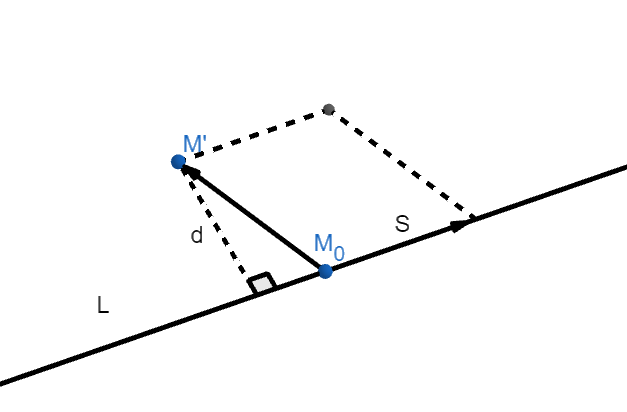
\includegraphics[width=5.5cm]{Images/Chapter_1/2-2-21.png}
        \end{center}
        \(d = |M', L| = \)

        \small\(= h(\)параллелограмма, построенного на \(\vec S\) и \(\overrightarrow{M_0 M'}) =\)\normalsize

        \(=\) \fbox{\(\dfrac{|\vec S \times \overrightarrow{M_0 M'}|}{|\vec S|}\)}
        \\
        \hline
        Полярное уравнение:
        \begin{center}
            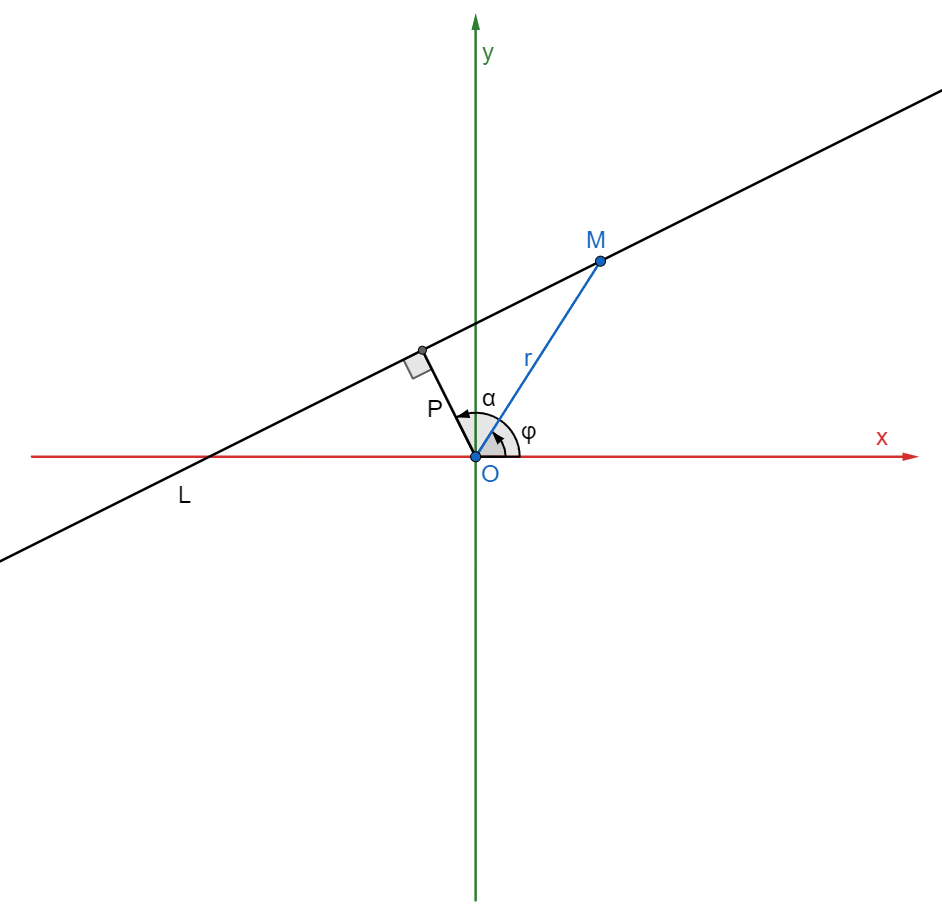
\includegraphics[width=5.5cm]{Images/Chapter_1/2-2-7.png}
        \end{center}
        \(O(0, 0) \notin L\)

        (Если \(O \in L\), то \(L\) распадается на 2 луча и точку \(O\))

        \(M(x, y) \in L\)

        \((x, y) \leftrightarrow (\varphi, r)\):

        \(
        \begin{cases}
            x = r \cos \varphi \\
            y = r \sin \varphi
        \end{cases}
        \)

        \(L\) задана нормальным уравнением:

        \small\(x \cos \alpha + y \sin \alpha - P = 0 \Leftrightarrow\)

        \scriptsize\(\Leftrightarrow r \cos \varphi \cos \alpha - r \sin \varphi \sin \alpha - P = 0 \Leftrightarrow\)

        \small\(\Leftrightarrow r \cos (\varphi - \alpha) - P = 0 \Leftrightarrow\)\normalsize

        \fbox{\(r = \dfrac{P}{\cos(\varphi - \alpha)}\)}

        \(r > 0\)

        \(P > 0\)

        \(\cos(\varphi - \alpha) > 0\)
         &
        \multicolumn{2}{p{11cm}}{

        Взаимное расположение прямой и плоскости в пространстве:

        \(\alpha: Ax + By + Cz + D = 0\), \(A^2 + B^2 + C^2 \neq 0\)

        \(L: \vec S = (l, m, n), M(x_0, y_0, z_0)\)

        \textbullet \(
        \left[\begin{array}{ll}
                  L \parallel \alpha \\
                  L \subset \alpha
              \end{array}\right .\)
        \(\Leftrightarrow \vec S \perp \vec N \Leftrightarrow \vec S \cdot \vec N = 0 \Leftrightarrow\)

        \(\)

        \(\Leftrightarrow Al + Bm + Cn = 0\)

        \textbullet \(L \subset \alpha \Leftrightarrow\)
        \(\begin{cases}
              \vec S \cdot \vec N = 0 \\
              M_0 \in \alpha
          \end{cases} \Leftrightarrow\)

        \(\Leftrightarrow
        \begin{cases}
            Al + Bm + Cn = 0 \\
            Ax_0 + By_0 + Cz_0 + D = 0
        \end{cases}\)

        \textbullet \(
        \begin{cases}
            L \parallel \alpha \\
            L \not\subset \alpha
        \end{cases} \Leftrightarrow
        \begin{cases}
            Al + Bm + Cn = 0 \\
            Ax_0 + By_0 + Cz_0 + D \neq 0
        \end{cases}\)

        \textbullet \(L \cap \alpha = Q\):
        \begin{center}
            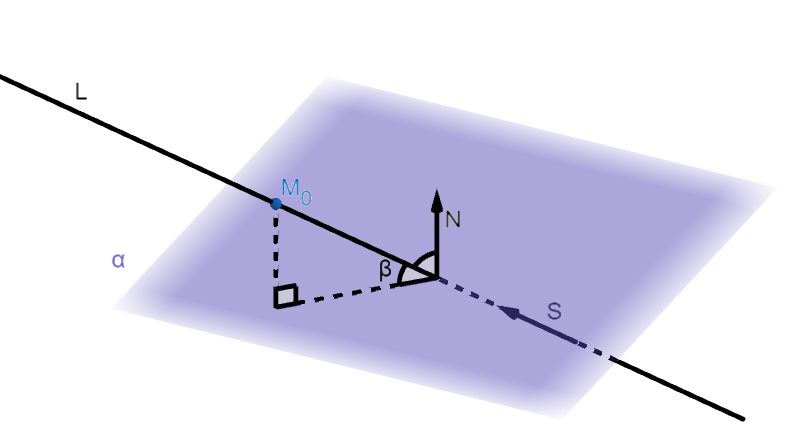
\includegraphics[width=7cm]{Images/Chapter_1/2-2-22.png}
        \end{center}
        \(Q(x_Q, y_Q, z_Q) \in L \Leftrightarrow
        \begin{cases}
            x_Q = x_0 + l t_Q \\
            y_Q = y_0 + m t_Q \\
            z_Q = z_0 + n t_Q
        \end{cases}\)

        \small\(Q \in \alpha \Leftrightarrow A(x_0 + l t_Q) + B(y_0 + m t_Q) + C(z_0 + n t_Q) + D = 0\)\normalsize

        \(\Leftrightarrow\)\fbox{\(t_Q = - \dfrac{Ax_0 + By_0 + Cz_0 + D}{Al + Bm + Cn}\)}

        \(\sin\angle(L, \alpha) = \cos(90^\circ - \angle(L, \alpha)) = \cos\angle(\vec N, \vec S) = \)

        \(=\) \fbox{\(\dfrac{\vec N \cdot \vec S}{|\vec N||\vec S|}\)}
        }\vline
        \\
        \hline
        Взаимное расположение прямых на плоскости:
        \textbullet \(L_1 \parallel L_2\):
        \begin{center}
            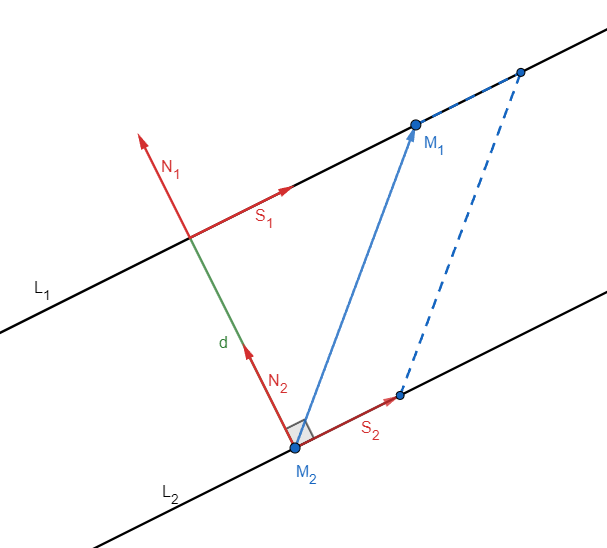
\includegraphics[width=5.5cm]{Images/Chapter_1/2-2-8.png}
        \end{center}
        \(L_1 \parallel L_2 \Leftrightarrow\)

        \(\Leftrightarrow \vec N_1 \parallel \vec N_2 \Leftrightarrow\)

        \(\Leftrightarrow \vec S_1 \parallel \vec S_2 \Leftrightarrow\)

        \(\Leftrightarrow\)\fbox{\(\dfrac{A_1}{A_2} = \dfrac{B_1}{B_2} \Leftrightarrow \dfrac{m_1}{m_2} = \dfrac{n_1}{n_2}\)}

        \(d = |L_1, L_2|\)(парам. ур.)\(=\)

        \small\(= h(\)параллелограмма, построенного на \(\vec S_2\) и \(\overrightarrow{M_2 M_1}) =\)\normalsize

        \(=\) \fbox{\(\dfrac{|\vec S_2 \times \overrightarrow{M_2 M_1}|}{|\vec S_2|}\)} \(=\)

        \(= |M_1, L_2|\)

        \textbullet \(L_1 = L_2 \Leftrightarrow\)

        \(\Leftrightarrow\)\fbox{\(\dfrac{A_1}{A_2} = \dfrac{B_1}{B_2} = \dfrac{C_1}{C_2}\)}

        \textbullet \(L_1 \cap L_2 = Q\):
        \begin{center}
            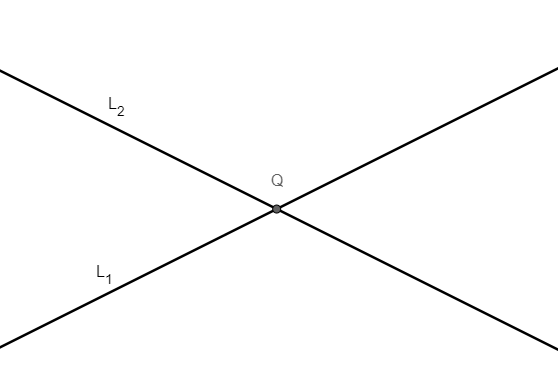
\includegraphics[width=5.5cm]{Images/Chapter_1/2-2-9.png}
        \end{center}
        \(L_1 \cap L_2 \Leftrightarrow \dfrac{A_1}{A_2} \neq \dfrac{B_1}{B_2}\)

        \small\(Q:
        \begin{cases}
            A_1 x + B_1 y + C_1 = 0 \\
            A_2 x + B_2 y + C_2 = 0
        \end{cases}
        \)\normalsize

        \(\Delta =
        \begin{vmatrix}
            A_1 & B_1 \\
            A_2 & B_2
        \end{vmatrix} =\)

        \(= A_1 B_2 - A_2 B_1 \neq 0 \Leftrightarrow\)

        \(\Leftrightarrow \exists ! \; Q\)
         &
        Взаимное расположение плоскостей в пространстве:

        \textbullet \(\alpha_1 \parallel \alpha_2\):
        \begin{center}
            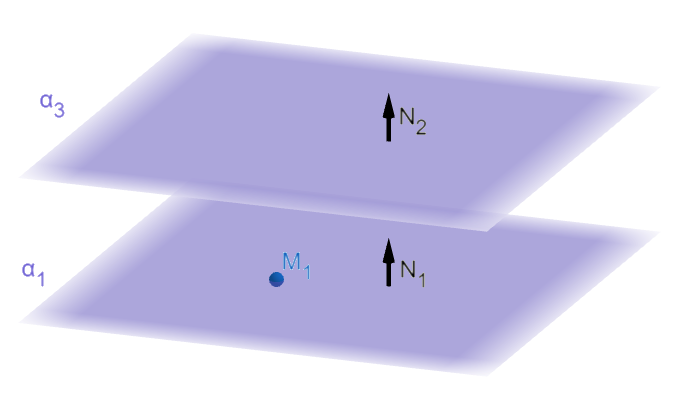
\includegraphics[width=5.5cm]{Images/Chapter_1/2-2-16.png}
        \end{center}
        \(\alpha_1 \parallel \alpha_2 \Leftrightarrow \vec N_1 \parallel \vec N_2 \Leftrightarrow\)

        \(\Leftrightarrow\) \fbox{\(\dfrac{A_1}{A_2} = \dfrac{B_1}{B_2} = \dfrac{C_1}{C_2}\)}

        \(d = |\alpha_1, \alpha_2|\)

        \(M_1 \in \alpha_1 \Rightarrow d = |M_1, \alpha_2|\)

        \(\alpha_1, \alpha_2\) заданы нормальным уравнением:

        \small\(d =
        \begin{cases}
            |P_1 - P_2|, \vec n_{0_1} = \vec n_{0_2} \\
            P_1 + P_2, \vec n_{0_1} = -\vec n_{0_2}  \\
        \end{cases}\)\normalsize

        \textbullet \(\alpha_1 = \alpha_2\):

        \fbox{\(\dfrac{A_1}{A_2} = \dfrac{B_1}{B_2} = \dfrac{C_1}{C_2} = \dfrac{D_1}{D_2}\)}

        \textbullet \(\alpha_1 \cap \alpha_2 = L\):
        \begin{center}
            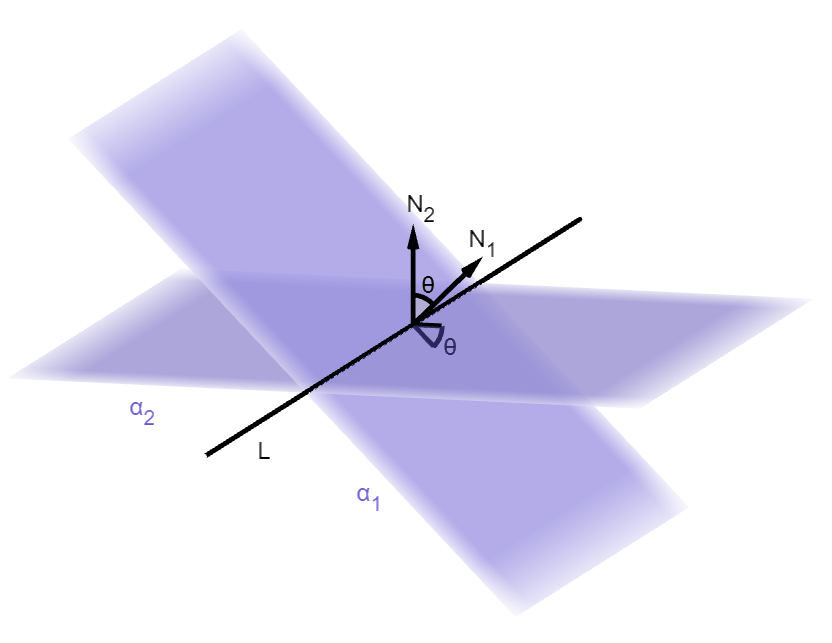
\includegraphics[width=5.5cm]{Images/Chapter_1/2-2-17.png}
        \end{center}
        \small\(L:\)

        \(\begin{cases}
              A_1 x + B_1 y + C_1 z + D_1 = 0 \\
              A_2 x + B_2 y + C_2 z + D_2 = 0
          \end{cases}\)\normalsize

        \(\Rightarrow
        \left[
        \begin{array}{lll}
            \dfrac{A_1}{A_2} \neq \dfrac{B_1}{B_2} \\
            \dfrac{B_1}{B_2} \neq \dfrac{C_1}{C_2} \\
            \dfrac{A_1}{A_2} \neq \dfrac{C_1}{C_2}
        \end{array}
        \right .\)

        \(\theta = \angle(\alpha_1, \alpha_2)\)

        \(|\cos\theta| = \dfrac{|\vec N_1 \cdot \vec N_2|}{|\vec N_1||\vec N_2|}\)
         &
        Взаимное расположение прямых в пространстве:

        \small\textbullet \(\left[
        \begin{array}{ll}
            L_1 \parallel L_2 \\
            L_1 = L_2
        \end{array}\right .\Leftrightarrow \vec S_1 \parallel \vec S_2 \Leftrightarrow\)\normalsize

        \(\Leftrightarrow\) \fbox{\(\dfrac{l_1}{l_2} = \dfrac{m_1}{m_2} = \dfrac{n_1}{n_2}\)}

        \small\textbullet\(L_1 = L_2 \Leftrightarrow
        \begin{cases}
            \vec S_1 \parallel \vec S_2 \\
            M_1 \in L_2
        \end{cases} \Leftrightarrow\)\normalsize

        \(\Leftrightarrow \vec S_1 \parallel \vec S_2 \parallel \overrightarrow{M_1 M_2} \Leftrightarrow\)

        \scriptsize\fbox{\(\Leftrightarrow
            \begin{cases}
                \dfrac{l_1}{l_2} = \dfrac{m_1}{m_2} = \dfrac{n_1}{n_2} \\
                \dfrac{l_1}{x_1 - x_2} = \dfrac{m_1}{y_1 - y_2} = \dfrac{n_1}{z_1 - z_2}
            \end{cases}\)}\normalsize

        \textbullet \(
        \begin{cases}
            L_1 \parallel L_2 \\
            L_1 \neq L_2
        \end{cases} \Leftrightarrow\)

        \(\Leftrightarrow
        \begin{cases}
            \vec S_1 \parallel \vec S_2 \\
            M_1 \notin L_2
        \end{cases}\Leftrightarrow\)

        \(\Leftrightarrow
        \begin{cases}
            \vec S_1 \parallel \vec S_2 \\
            \vec S_1 \nparallel \overrightarrow{M_1 M_2}
        \end{cases}\)

        \(d = |L_1, L_2| = |M_1, L_2| =\)

        \(= \dfrac{|\vec S \times \overrightarrow{M_1 M_2}|}{|\vec S|}\)

        \textbullet\(L_1 \cap L_2 = Q \Leftrightarrow\)

        \(\Leftrightarrow\)\fbox{\(
            \begin{cases}
                \vec S_1 \nparallel \vec S_2 \\
                \vec S_1 \vec S_2 \overrightarrow{M_1 M_2} = 0
            \end{cases}\)}

        \(\cos\angle(L_1, L_2) = \dfrac{\vec S_1 \cdot \vec S_2}{|\vec S_1||\vec S_2|}\)

        \textbullet \(L_1 \skewed L_2:\)

        \begin{center}
            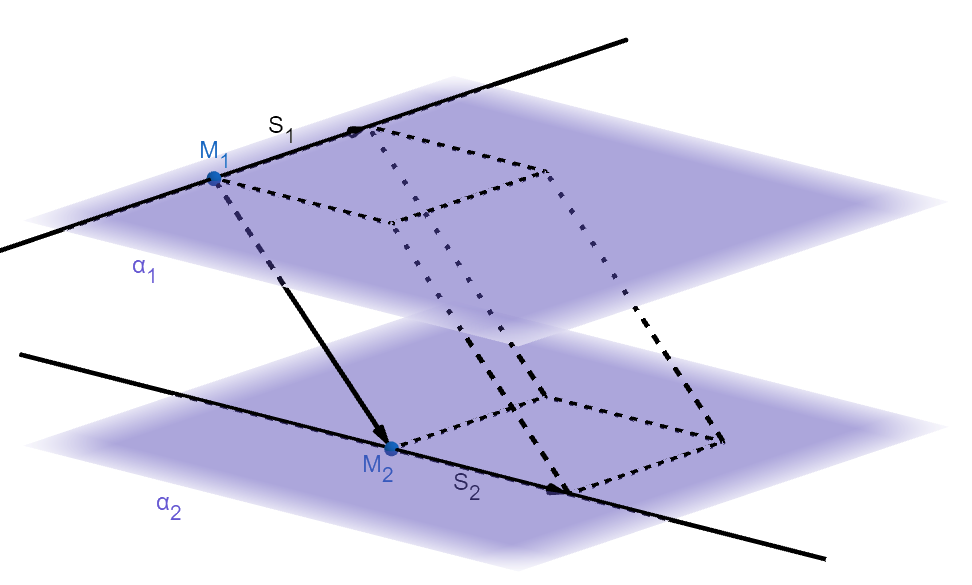
\includegraphics[width=5.5cm]{Images/Chapter_1/2-2-23.png}
        \end{center}

        \(\vec S_1 \vec S_2 \overrightarrow{M_1 M_2} \neq 0 \Rightarrow\)

        \(\Rightarrow \exists \alpha_1, \alpha_2:
        \begin{cases}
            \alpha_1 \parallel \alpha_2 \\
            L_1 \subset \alpha_1        \\
            L_2 \subset \alpha_2
        \end{cases}\)
        \\ & &
        \(|L_1, L_2| = |\alpha_1, \alpha_2| = h(\)параллелепипед, построенный на \(\vec S_1, \vec S_2, \overrightarrow{M_1 M_2}) = \)

        \(=\)\fbox{\(\dfrac{|\vec S_1 \vec S_2 \overrightarrow{M_1 M_2}|}{|\vec S_1 \times \vec S_2|}\)}

        \begin{center}
            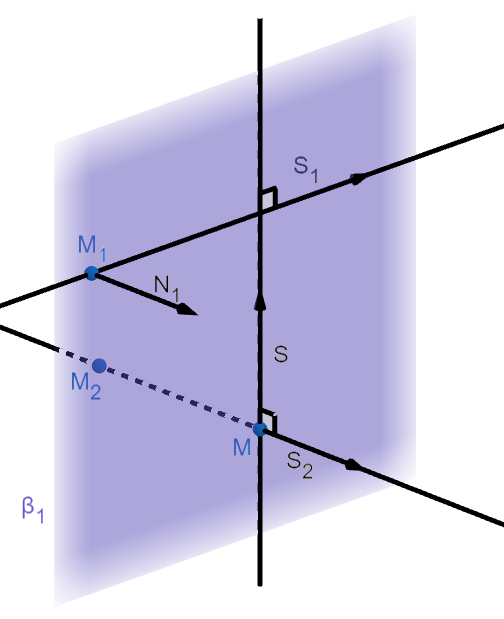
\includegraphics[width=5.5cm]{Images/Chapter_1/2-2-24.png}
        \end{center}
        \(L(M, \vec S):
        \begin{cases}
            L \perp L_1 \\
            L \perp L_2
        \end{cases}\)

        \(\vec S = \vec S_1 \times \vec S_2\)

        \(\beta_1(\vec S_1, \vec S, M_1) \Rightarrow\)

        \(\Rightarrow\)\fbox{\(M = L_2 \cap \beta_1\)}

        \(\vec N_1 = \vec S_1 \times \vec S =\)

        \(= \vec S_1 \times (\vec S_1 \times \vec S_2)\)
        \\
        \hline
    \end{longtable}
\end{center}


\subsection{Проекция точки на плоскость и прямую}
\begin{center}
    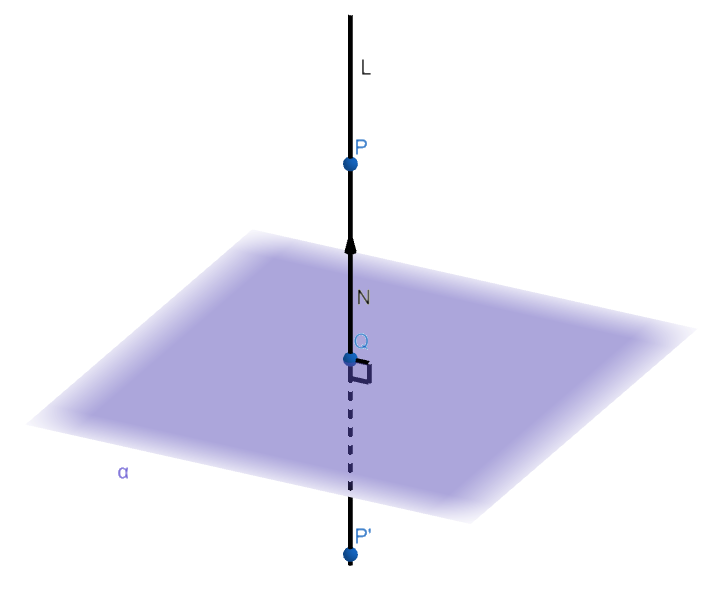
\includegraphics[height=7cm]{Images/Chapter_1/2-3-1.png}
\end{center}
\(PQ \perp \alpha\), \(Q \in \alpha\)

\(\alpha: Ax + By + Cz + D = 0\), \(\vec N = (A, B, C)\)

\(P(P_1, P_2, P_3)\)

\(L(P, \vec N):
\begin{cases}
    x = P_1 + t A \\
    y = P_2 + t B \\
    z = P_3 + t C
\end{cases} \Rightarrow Q = L \cap \alpha \Rightarrow\)

\(\Rightarrow A(P_1 + t_Q A) + B(P_2 + t_Q B) + C(P_3 + t_Q C) + D = 0 \Rightarrow\)\fbox{\(t_Q = - \dfrac{AP_1 + BP_2 + CP_3 + D}{A^2 + B^2 + C^2}\)}

\(P'\) --- отражение \(P\) относительно \(\alpha \Rightarrow P' = 2Q - P\)
\begin{center}
    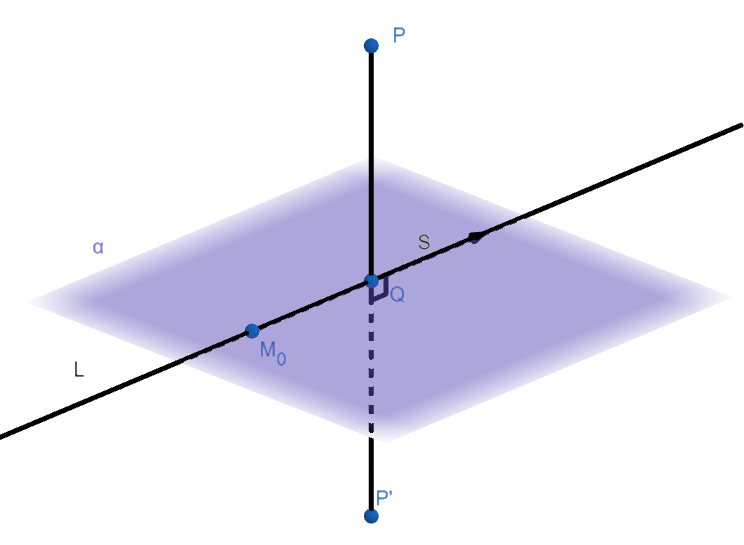
\includegraphics[height=7cm]{Images/Chapter_1/2-3-2.png}
\end{center}
\(PQ \perp L(M_0, \vec S = (l, m, n))\), \(Q \in L\)

\(P = (P_1, P_2, P_3)\)

\(\alpha(P, \vec S): l(x - P_1) + m(y - P_2) + n(z - P_3) = 0\)
\(L:
\begin{cases}
    x = x_0 + t l \\
    y = y_0 + t m \\
    z = z_0 + t n
\end{cases}\)

\(Q = \alpha \cap L \Rightarrow l((x_0 + t_Q l) - P_1) + m((y_0 + t_Q m) - P_2) + n((z_0 + t_Q n) - P_3) = 0\)

Находим из этого \(t_Q\) и подставляем в уравнение \(L\).

\(P'\) --- отражение \(P\) относительно \(L \Rightarrow P' = 2Q - P\)


\section{Кривые второго порядка (КВП)}
\subsection{Канонические уравнения КВП}
Кривая второго порядка --- множество точек на плоскости, декартовы координаты которых удовлетворяет алгебраическому уравнению 2-го порядка:

\(a_{11} x^2 + 2 a_{12} xy + a_{22} y^2 + 2 a_1 x + 2 a_2 y + a_0 = 0\), \((a_{11}^2 + a_{12}^2 + a_{22}^2 \neq 0)\)

КВП делятся на 2 вида:
\begin{enumerate}
    \item Невырожденные:
          \begin{itemize}
              \item Эллипс
              \item Парабола
              \item Гипербола
          \end{itemize}
    \item Вырожденные:
          \begin{itemize}
              \item Пара пересекающихся прямых
              \item Пара параллельных прямых
              \item Пара совпадающих прямых
              \item Точка
              \item Пустое множество
          \end{itemize}
\end{enumerate}

\begin{center}
    \begin{longtable}{|p{2.5cm}|p{4.5cm}|p{4.5cm}|p{4.5cm}|}
        \hline
         &
        Эллипс
         &
        Гипербола
         &
        Парабола
        \\
        \hline
        Опр. 1
         &
        ГМТ на плоскости, таких, что сумма расстояний до двух фиксированных точек плоскости --- величина постоянная и равная \(2a\).
        \begin{center}
            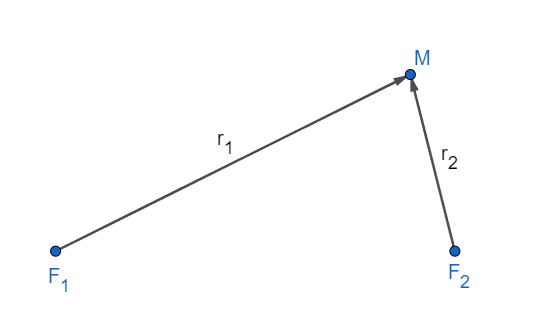
\includegraphics[width=4.5cm]{Images/Chapter_1/3-1-1.png}
        \end{center}
        \(r_1 + r_2 = 2a = \mathbf{const}\)
         &
        ГМТ на плоскости, таких, что модуль разности расстояний до двух фиксированных точек плоскости --- величина постоянная и равная \(2a\).
        \begin{center}
            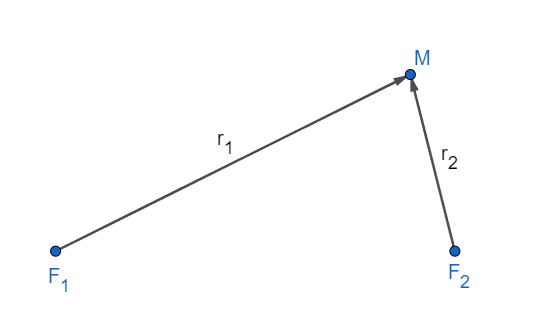
\includegraphics[width=4.5cm]{Images/Chapter_1/3-1-1.png}
        \end{center}
        \(|r_1 - r_2| = 2a = \mathbf{const}\)
         &
        ГМТ на плоскости, таких, что расстояние до фиксированной точки плоскости равно расстоянию до фиксированной прямой.
        \begin{center}
            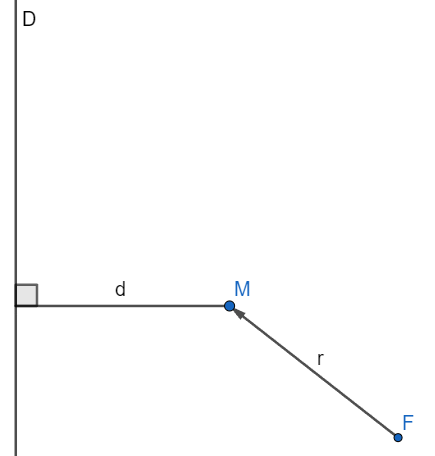
\includegraphics[width=4.5cm]{Images/Chapter_1/3-1-2.png}
        \end{center}
        \(r = d\)
        \\
        \hline
        Уравнение в ДСК
         &
        \begin{center}
            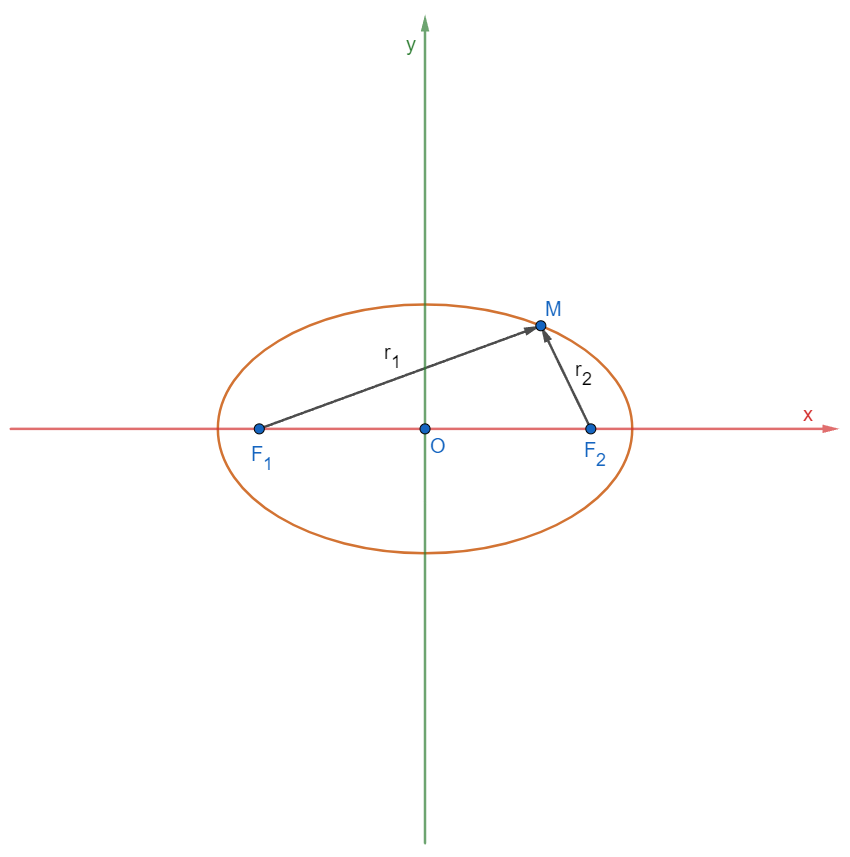
\includegraphics[width=4.5cm]{Images/Chapter_1/3-1-3.png}
        \end{center}
        \(F_{1, 2}\) --- фокусы

        \(F_1(-c, 0)\), \(F_2(c, 0)\)

        \fbox{\(\dfrac{x^2}{a^2} + \dfrac{y^2}{b^2} = 1\)}

        \(a^2 = b^2 + c^2\), \(a > c\)

        \(r_1, r_2\) --- фокальные радиусы

        \(a\) --- большая полуось

        \(b\) --- малая полуось
         &
        \begin{center}
            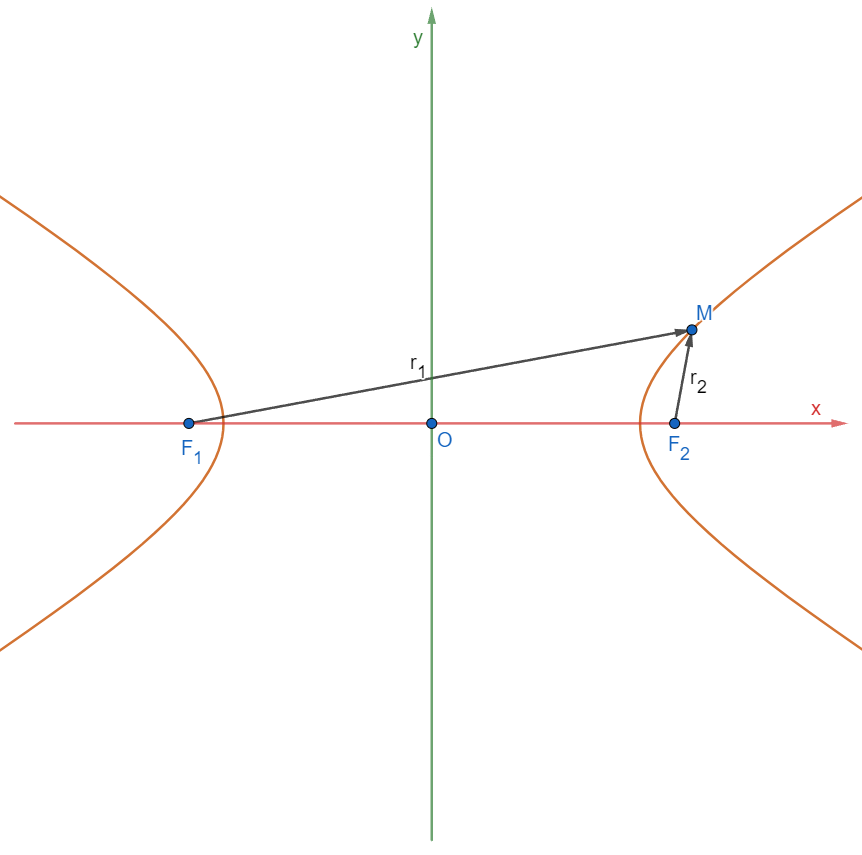
\includegraphics[width=4.5cm]{Images/Chapter_1/3-1-4.png}
        \end{center}
        \(F_{1, 2}\) --- фокусы

        \(F_1(-c, 0)\), \(F_2(c, 0)\)

        \fbox{\(\dfrac{x^2}{a^2} - \dfrac{y^2}{b^2} = 1\)}

        \(c^2 = a^2 + b^2\), \(a < c\)

        \(r_1, r_2\) --- фокальные радиусы

        \(a\) --- действительная полуось

        \(b\) --- мнимая полуось

        Имеет асимптоты --- \(y = \pm \dfrac{b}{a} x\)

        \(\)
         &
        \begin{center}
            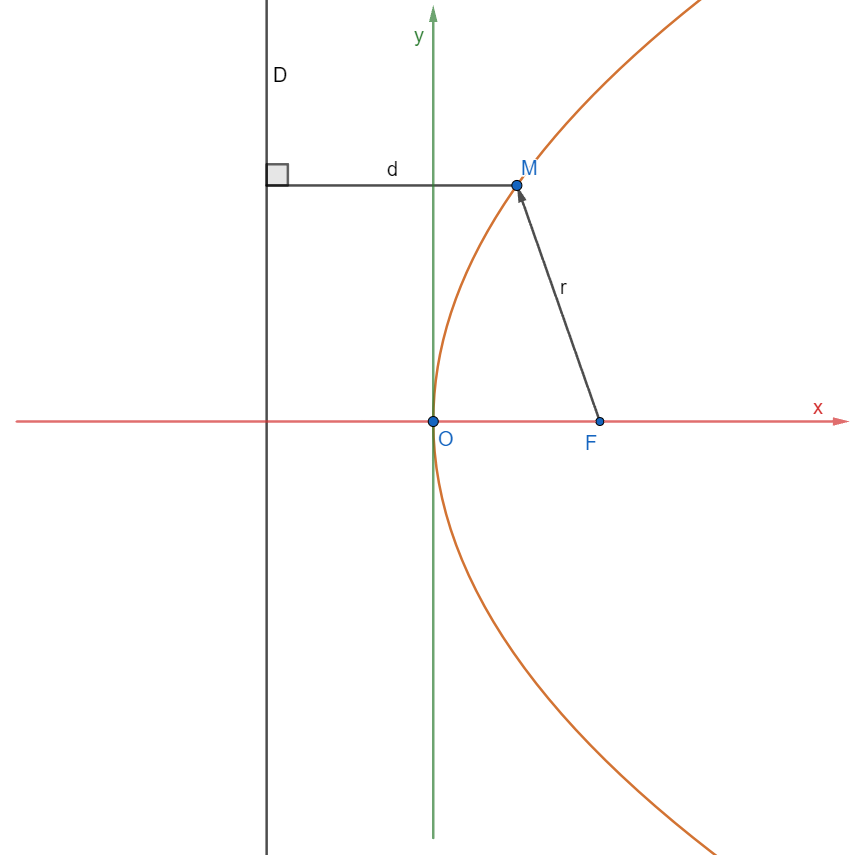
\includegraphics[width=4.5cm]{Images/Chapter_1/3-1-5.png}
        \end{center}
        \(F\) --- фокус, \(D\) --- директриса

        \(F\left(\dfrac{p}{2}, 0\right)\), \(D: x = -\dfrac{p}{2}\)

        \fbox{\(y^2 = 2px\)}

        \(p = |F, D|\)

        \(p\) --- фокальный параметр
        \\
        \hline
        \(\varepsilon\) --- Эксцентриситет
         &
        \(\varepsilon = \dfrac{c}{a} < 1\)
         &
        \(\varepsilon = \dfrac{c}{a} > 1\)
         &
        \(\varepsilon = 1\)
        \\
        \hline
        \(r_{1, 2}\) --- фокальные радиусы
         &
        \(r_{1, 2} = a \pm \varepsilon x\)

        \(M(x, y) \in\) эллипсу
         &
        Правая ветвь:

        \(r_{1, 2} = \varepsilon x \pm a\)

        Левая ветвь:

        \(r_{1, 2} = -\varepsilon x \mp a\)

        \(M(x, y) \in\) гиперболе
         &
        \(r = x + \dfrac{p}{2}\)
        \\
        \hline
        Директрисы
         &
        \begin{center}
            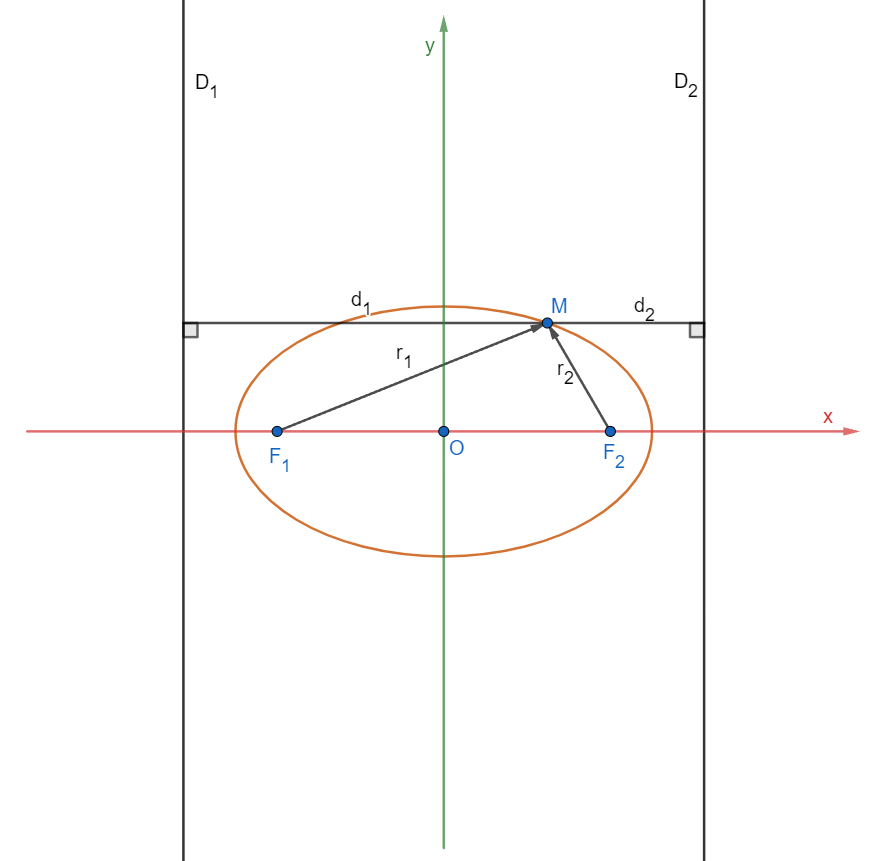
\includegraphics[width=4.5cm]{Images/Chapter_1/3-1-6.png}
        \end{center}
        \(D_{1, 2}: x = \mp \dfrac{a}{\varepsilon}\)

        \(\dfrac{r_1}{d_1} = \dfrac{r_2}{d_2} = \varepsilon = \dfrac{r}{d}\)
         &
        \begin{center}
            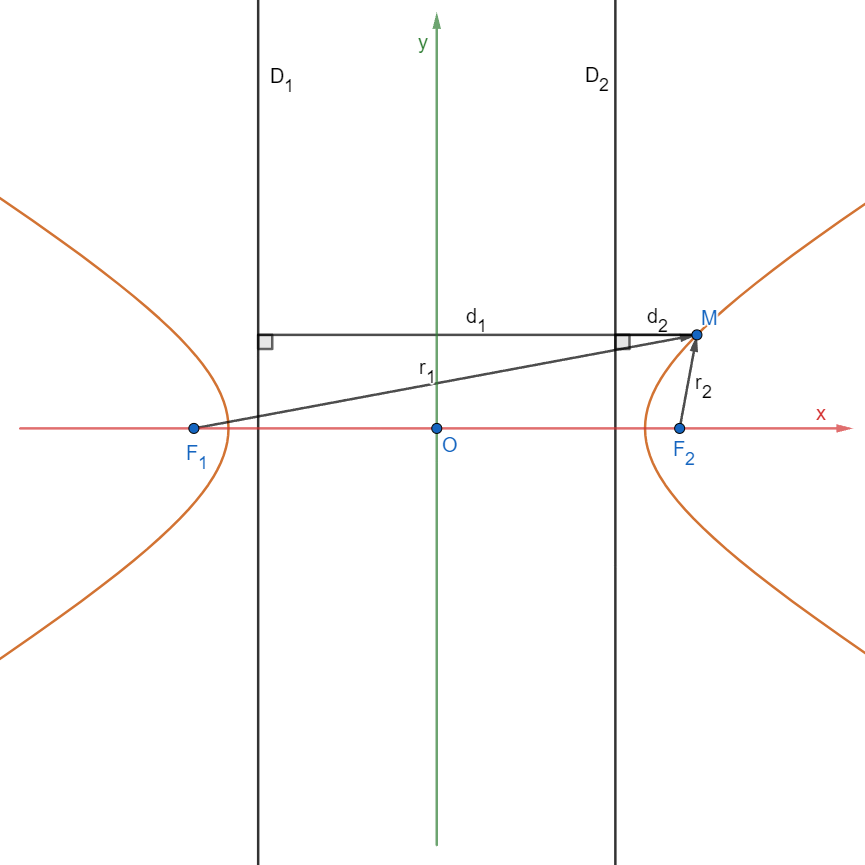
\includegraphics[width=4.5cm]{Images/Chapter_1/3-1-7.png}
        \end{center}
        \(D_{1, 2}: x = \mp \dfrac{a}{\varepsilon}\)

        \(\dfrac{r_1}{d_1} = \dfrac{r_2}{d_2} = \varepsilon = \dfrac{r}{d}\)
         &
        \(\dfrac{r}{d} = 1 = \varepsilon\)
        \\
        \hline
        Опр. 2
         &
        ГМТ на плоскости, таких, что отношение расстояния до фиксированной точки плоскости к расстоянию до прямой --- величина постоянная и меньшая единицы.

        \(\varepsilon = \mathbf{const} = \dfrac{r}{d} < 1\)
        \begin{center}
            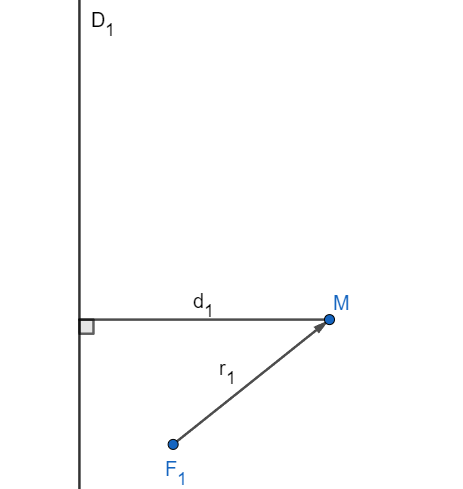
\includegraphics[width=4.5cm]{Images/Chapter_1/3-1-8.png}
        \end{center}
         &
        ГМТ на плоскости, таких, что отношение расстояния до фиксированной точки плоскости к расстоянию до прямой --- величина постоянная и большая единицы.

        \(\varepsilon = \mathbf{const} = \dfrac{r}{d} > 1\)
        \begin{center}
            \includegraphics[width=4.5cm]{Images/Chapter_1/3-1-9.png}
        \end{center}
         &
        ГМТ на плоскости, таких, что отношение расстояния до фиксированной точки плоскости к расстоянию до прямой --- величина постоянная и равная единице.

        \(\varepsilon = \mathbf{const} = \dfrac{r}{d} = 1\)
        \begin{center}
            \includegraphics[width=4.5cm]{Images/Chapter_1/3-1-2.png}
        \end{center}
        \\
        \hline
        Полярное уравнение
         &
        \begin{center}
            \includegraphics[width=4.5cm]{Images/Chapter_1/3-1-10.png}
        \end{center}
        Начало ПСК в одном из фокусов, ось направлена в сторону соответствующей директрисы.

        \(r = \dfrac{P}{1 + \varepsilon \cos\varphi}\)

        \(P\) --- фокальный параметр.

        \(P = \varepsilon \cdot q = \dfrac{b^2}{a}\)

        \(q = |F, D| = \dfrac{a}{\varepsilon} - c\)

        \(P\) --- Длина перпендикуляра от \(F\) до эллипса

        Директрисы:

        \(r = \dfrac{\pm \dfrac{a}{\varepsilon} - c}{\cos\varphi}\)

        Если ось направлена в противоположную сторону, то меняем знак косинуса.
         &
        \begin{center}
            \includegraphics[width=4.5cm]{Images/Chapter_1/3-1-11.png}
        \end{center}
        Начало ПСК в одном из фокусов, ось направлена в сторону соответствующей директрисы.

        \(r = \dfrac{\pm P}{1 \pm \varepsilon \cos\varphi}\)

        Ветвь, более близкая к фокусу: \(``+"\)

        Ветвь, более далёкая от фокуса: \(``-"\)

        \(P\) --- фокальный параметр.

        \(P = \varepsilon \cdot q = \dfrac{b^2}{a}\)

        \(q = |F, D| = c - \dfrac{a}{\varepsilon}\)

        \(P\) --- Длина перпендикуляра от \(F\) до гиперболы.

        Директрисы:

        \(r = \dfrac{\pm \dfrac{a}{\varepsilon} + c}{\cos\varphi}\)

        Если ось направлена в противоположную сторону, то меняем знак косинуса.
         &
        \begin{center}
            \includegraphics[width=4.5cm]{Images/Chapter_1/3-1-12.png}
        \end{center}
        Начало ПСК в фокусе, ось направлена в сторону директрисы.

        \(r = \dfrac{P}{1 + \varepsilon \cos\varphi} = \)

        \(= \dfrac{P}{1 + \cos\varphi}\)

        \(P\) --- Длина перпендикуляра от \(F\) до параболы

        Если ось направлена в противоположную сторону, то меняем знак косинуса.
        \\
        \hline
        Касательные
         &
        \begin{center}
            \includegraphics[width=4.5cm]{Images/Chapter_1/3-1-13.png}
        \end{center}
        \(M(x_0, y_0) \in\) эллипсу

        \(\dfrac{x x_0}{a^2} + \dfrac{y y_0}{b^2} = 1\)
         &
        \begin{center}
            \includegraphics[width=4.5cm]{Images/Chapter_1/3-1-14.png}
        \end{center}
        \(M(x_0, y_0) \in\) гиперболе

        \(\dfrac{x x_0}{a^2} - \dfrac{y y_0}{b^2} = 1\)
         &
        \begin{center}
            \includegraphics[width=4.5cm]{Images/Chapter_1/3-1-15.png}
        \end{center}
        \(M(x_0, y_0) \in\) параболе

        \(y y_0 = P(x + x_0)\)
        \\
        \hline
        Оптические свойства
         &
        \begin{center}
            \includegraphics[width=4.5cm]{Images/Chapter_1/3-1-16.png}
        \end{center}
        Любой луч, вышедший из одного фокуса, отразившись, пройдёт через другой фокус.
         &
        \begin{center}
            \includegraphics[width=4.5cm]{Images/Chapter_1/3-1-17.png}
        \end{center}
        Любой луч, вышедший из одного фокуса, отразившись, пройдёт по прямой, проходящей через другой фокус.
         &
        \begin{center}
            \includegraphics[width=4.5cm]{Images/Chapter_1/3-1-18.png}
        \end{center}
        Любой луч, вышедший из фокуса, отразившись, пройдёт по прямой, параллельной оси параболы.
        \\
        \hline
        Другие свойства
         &
        \begin{center}
            \includegraphics[width=4.5cm]{Images/Chapter_1/3-1-19.png}
        \end{center}
        \(\dfrac{MN}{M'N} = \dfrac{b}{a}\)

        Любой эллипс --- сжатая по какой-то оси окружность.
         &
        \begin{center}
            \includegraphics[width=4.5cm]{Images/Chapter_1/3-1-20.png}
        \end{center}
        \(\dfrac{y^2}{b^2} - \dfrac{x^2}{a^2} = 1\) --- сопряжённая гипербола. Имеет те же асимптоты.
         &

        \\
        \hline
    \end{longtable}
\end{center}
Доказательство свойств (на примере гиперболы, эллипс доказывается полностью аналогично):
\begin{itemize}
    \item Каноническое уравнение

          По определению: \(|r_1 - r_2| = 2a\)

          \(F_1(-c, 0)\), \(F_2(c, 0)\), \(c > a\)

          \(r_1 = \sqrt{(x + c)^2 + y^2}\), \(r_2 = \sqrt{(x - c)^2 + y^2}\)

          Пусть \(r_1 > r_2\) (правая ветвь) \(\Rightarrow r_1 = 2a + r_2 \Rightarrow r_1^2 = 4a^2 + 4ar_2 + r_2^2 \Rightarrow\)

          \(\Rightarrow (x + c)^2 + y^2 = 4a^2 + 4ar_2 + (x - c)^2 + y^2 \Rightarrow xc = a^2 + ar_2 \Rightarrow r_2 = \dfrac{xc}{a} - a\)

          \(\varepsilon = \dfrac{c}{a} \Rightarrow\) \fbox{\(r_2 = x \varepsilon - a\)} --- зависимость фокального радиуса от \(x\)

          \(r_2^2 = (x - c)^2 + y^2 \Rightarrow (x - c)^2 + y^2 = \dfrac{x^2 c^2}{a^2} - 2xc + a^2 \Rightarrow x^2\left(1 - \dfrac{c^2}{a^2}\right) + y^2 = a^2 - c^2 \Rightarrow\)

          \(\Rightarrow \dfrac{x^2(a^2 - c^2)}{a^2} + y^2 = a^2 - c^2 \Rightarrow \dfrac{x^2}{a^2} - \dfrac{y^2}{c^2 - a^2} = 1 \Rightarrow\) \fbox{\(\dfrac{x^2}{a^2} - \dfrac{y^2}{b^2} = 1\)} \(Q.E.D.\)

          Из \(r_2 = -2a + r_1\) аналогично можно получить \(r_1 = x \varepsilon + a\). Значит \fbox{\(r_{1, 2} = x \varepsilon \pm a\)}

          Если \(r_1 < r_2\) (левая ветвь): \fbox{\(r_{1, 2} = -x \varepsilon \mp a\)}

    \item Директрисы:

          \(D_2: x = \pm \dfrac{a}{\varepsilon}\), \(d_2 = |M, D_2| = \left|x - \dfrac{a}{\varepsilon}\right|\)

          Правая ветвь: \(r_2 = x \varepsilon - a \Rightarrow \dfrac{r_2}{d_2} = \dfrac{x \varepsilon - a}{x - \dfrac{a}{\varepsilon}} = \varepsilon \dfrac{x - \dfrac{a}{\varepsilon}}{x - \dfrac{a}{\varepsilon}} = \varepsilon\)

          Левая ветвь: \(r_2 = -x \varepsilon + a \Rightarrow \dfrac{r_2}{d_2} = \dfrac{-x \varepsilon + a}{-x + \dfrac{a}{\varepsilon}} = \varepsilon \dfrac{-x + \dfrac{a}{\varepsilon}}{-x + \dfrac{a}{\varepsilon}} = \varepsilon\)

          \(\dfrac{r_2}{d_2} = \varepsilon \Rightarrow D_2\) --- директриса \(Q.E.D.\)

          Для \(r_1\) и \(D_1\) заменить \(x\) на \(-x\)

    \item Определение 2:

          Пусть известно \(Q = |F, D|\) и \(\varepsilon = \dfrac{r}{d} > 1\)

          Проведём ДСК, в которой \(D \parallel Oy\). Давайте найдём параметры канонического уравнения, считая, что \(D: x = \dfrac{a}{\varepsilon}\), а \(F = (c, 0)\).

          \(\begin{rcases}
              c - \dfrac{a}{\varepsilon} = Q \\
              \dfrac{c}{a} = \varepsilon
          \end{rcases} \Rightarrow c = Q + \dfrac{a}{\varepsilon} \Rightarrow a \varepsilon = Q + \dfrac{a}{\varepsilon} \Rightarrow a \left(\varepsilon - \dfrac{1}{\varepsilon}\right) = Q \Rightarrow\) \fbox{\(a = \dfrac{\varepsilon Q}{\varepsilon^2 - 1}\)} \(\Rightarrow\)

          \(\Rightarrow\) \fbox{\(c = \dfrac{\varepsilon^2 Q}{\varepsilon^2 - 1}\)}

          Мы в узнали чему равны \(a\) и \(c\) из известных нам \(\varepsilon\) и \(Q\), значит точки, удовлетворяющие 2-му определению, удовлетворяют \(\dfrac{x^2}{a^2} - \dfrac{y^2}{b^2} = 1\), а \(D\) --- очевидно директриса гиперболы. \(Q.E.D.\)

    \item Асимптоты:

          Найдём \(y(x)\) для I координатной четверти: \(\dfrac{x^2}{a^2} - \dfrac{y^2}{b^2} = 1 \Rightarrow y = b \sqrt{\dfrac{x^2}{a^2} - 1}\)

          Найдём угловой коэффициент асимптоты \(k = \lim\limits_{x \to +\infty}\dfrac{y(x)}{x}\):

          \(k = \lim\limits_{x \to +\infty} \dfrac{b \sqrt{\dfrac{x^2}{a^2} - 1}}{x} = \lim\limits_{x \to +\infty} \dfrac{b x \sqrt{\dfrac{1}{a^2} - \dfrac{1}{x^2}}}{x} = \dfrac{b}{a}\)

          Найдём ординату пересечения асимптоты и оси ординат \(m = \lim\limits_{x \to +\infty}(y(x) - kx)\):

          \(\lim\limits_{x \to +\infty} \left(b \sqrt{\dfrac{x^2}{a^2} - 1} - \dfrac{b}{a}x\right) = b \lim\limits_{x \to +\infty} \left(\sqrt{\dfrac{x^2}{a^2} - 1} - \dfrac{x}{a}\right) =\)

          \(=b \lim\limits_{x \to +\infty} \left(\dfrac{\dfrac{x^2}{a^2} - 1 - \dfrac{x^2}{a^2}}{\sqrt{\dfrac{x^2}{a^2} - 1} + \dfrac{x}{a}} \right) = b \lim\limits_{x \to +\infty} \left(\dfrac{-1}{\sqrt{\dfrac{x^2}{a^2} - 1} + \dfrac{x}{a}} \right) = 0\)

          Значит асимптота: \(y = \dfrac{b}{a} x\)

          По симметрии получаем \(y = \pm \dfrac{b}{a} x\) \(Q.E.D.\)

    \item Полярное уравнение:

          Зададим ПСК\((r, \varphi)\), у которой полюс \(O'= F_2 = (c, 0)\), а ось направлена в сторону \(-x\).

          \(x = c - r \cos \varphi\)

          Правая ветвь: \(r = r_2 = x \varepsilon - a\)

          \(r = \varepsilon(c - r \cos \varphi) - a = \varepsilon c - \varepsilon r \cos \varphi - a \Rightarrow r(1 + \varepsilon \cos \varphi) = \varepsilon c - a = \varepsilon \left(c - \dfrac{a}{\varepsilon}\right) = P \Rightarrow r = \dfrac{P}{1 + \varepsilon \cos \varphi}\)

          Левая ветвь: \(r = r_2 = - x \varepsilon + a\)

          \(r = - \varepsilon(c - r \cos \varphi) + a = - \varepsilon c + \varepsilon r \cos \varphi + a \Rightarrow r(1 - \varepsilon \cos \varphi) = a - \varepsilon c = \varepsilon \left(\dfrac{a}{\varepsilon} - c\right) = -P \Rightarrow r = \dfrac{-P}{1 - \varepsilon \cos \varphi}\)

          Если ось направлена в противоположную сторону, то \(\cos(2 \pi - \varphi) = - \cos \varphi\), и \(\cos \varphi\) в формулы записывается со знаком минус.

          Аналогично, если у ПСК полюс в \(F_1\).

    \item Касательные

          Формула касательной к функции в точке \(M_0(x_0, y_0)\): \(y = f'(x_0)(x - x_0) + y_0\)

          \(\dfrac{x^2}{a^2} - \dfrac{y^2}{b^2} = 1 \Rightarrow \dfrac{x^2}{a^2} - \dfrac{f(x)^2}{b^2} = 1 \Rightarrow (\)Возьмём производную обеих сторон\() \Rightarrow\)

          \(\Rightarrow \dfrac{2x}{a^2} - \dfrac{2 f(x) f'(x)}{b^2} = 0 \Rightarrow \dfrac{2 f(x) f'(x)}{b^2} = \dfrac{2x}{a^2}\)

          Подставим \(x_0\): \(\dfrac{2 f(x_0) f'(x_0)}{b^2} = \dfrac{2x_0}{a^2} \Rightarrow \dfrac{y_0 f'(x_0)}{b^2} = \dfrac{x_0}{a^2} \Rightarrow f'(x_0) = \dfrac{x_0 b^2}{y_0 a^2}\)

          Подставим в формулу для касательной: \(y = \dfrac{x_0 b^2}{y_0 a^2}(x - x_0) + y_0=\)

          \(= \dfrac{x_0 b^2 (x - x_0) + y_0^2 a^2}{y_0 a^2} \Rightarrow\)

          \(\Rightarrow y y_0 a^2 = x x_0 b^2 - x_0^2 b^2 + y_0^2 a^2 \Rightarrow \dfrac{x x_0}{a^2} - \dfrac{y y_0}{b^2} = \dfrac{x_0^2}{a^2} - \dfrac{y_0^2}{b^2} = 1\) \(Q.E.D.\)

    \item Оптические свойства

          Пусть \(M_0(x_0, y_0)\) лежит на гиперболе. Тогда:

          \(\vec r_1 = \overrightarrow{F_1 M_0} = (x_0 + c, y_0)\), \(\vec r_2 = \overrightarrow{F_2 M_0} = (x_0 - c, y_0)\)

          Проверим, что биссектриса между \(\vec r_1\) и \(\vec r_2\) параллельна касательной в точке \(M_0\), то есть перпендикулярна перпендикуляру касательной \(\vec N = \left(\dfrac{x_0}{a^2}, -\dfrac{y_0}{b^2}\right)\).

          Биссектриса между \(\vec r_1\) и \(\vec r_2\): \(|\vec r_1|\vec r_2 + |\vec r_2| \vec r_1 = (\varepsilon x_0 + a) \vec r_2 + (\varepsilon x_0 - a) \vec r_1 =\)

          \(=((x_0 - c)(\varepsilon x_0 + a) + (\varepsilon x_0 - a)(x_0 + c), y_0(\varepsilon x_0 + a) + y_0(\varepsilon x_0 - a)) =\)

          \(= (2\varepsilon x_0^2 - 2ac, 2 \varepsilon x_0 y_0) \sim \left(x_0^2 - \dfrac{ac}{\varepsilon}, x_0 y_0\right)\)

          Скалярно перемножим с \(\vec N\): \(\left(x_0^2 - \dfrac{ac}{\varepsilon}\right)\dfrac{x_0}{a^2} - x_0 y_0 \dfrac{y_0}{b^2} = \dfrac{x_0^3}{a^2} - \dfrac{x_0 c}{\varepsilon a} - \dfrac{x_0 y_0^2}{b^2} =\)

          \(= x_0 \left(\dfrac{x_0^2}{a^2} - \dfrac{y_0^2}{b^2}\right) - x_0 = x_0 - x_0 = 0 \Rightarrow N \perp\) биссектрисе \(Q.E.D.\)
\end{itemize}

\subsection{Приведение КВП к каноническому виду}
\(a_{11} x^2 + 2 a_{12} x y + a_{22} y^2 + 2 a_1 x + 2 a_2 y + a_0 = 0\), \(a_{11}^2 + a_{12}^2 + a_{22}^2 \neq 0\)

Очевидно, что КВП не меняет своего типа при повороте и сдвиге.

\begin{enumerate}
    \item Если \(a_{12} \neq 0\), подберём такой угол поворота \(\alpha\), чтобы в новом уравнении \(a_{12}' = 0\).

          Выразим старые координаты через новые:

          \(x = x' \cos \alpha - y' \sin \alpha\), \(y = x' \sin \alpha + y' \cos \alpha\), \(\alpha \in \left(-\dfrac{\pi}{2}, \dfrac{\pi}{2}\right) \setminus \{0\}\)

          Выразим \(a_{12}'\) через старые коэффициенты, \(\sin \alpha = S_\alpha\) и \(\cos \alpha = C_\alpha\) и приравняем к \(0\):

          \(a_{12} = -2 a_{11} C_\alpha S_\alpha + 2 a_{12} (C_\alpha^2 S_\alpha^2) + 2 a_{22} C_\alpha S_\alpha = 0\)

          \((a_{22} - a_{11}) \tan \alpha + a_{12} (1 - \tan^2 \alpha) = 0\)

          \(\tan^2 \alpha + \dfrac{a_{22} - a_{11}}{a_{12}} \tan \alpha - 1 = 0\) ~--- квадратное уравнение относительно \(\tan \alpha\)

          Дискриминант \(D = \left(\dfrac{a_{22} - a_{11}}{a_{12}}\right) ^ 2 + 4 > 0\) ~--- 2 решения

          По теореме Виета \(\tan \alpha_1 \cdot \tan \alpha_2 = -1 \Rightarrow \alpha_1 \in \left(0, \dfrac{\pi}{2}\right)\), \(\alpha_2 \in \left(-\dfrac{\pi}{2}, 0\right)\), \(\alpha_1 - \alpha_2 = 90^\circ\)

          \(\alpha_{1, 2} = \arctan\left(\dfrac{-\dfrac{a_{22} - a_{11}}{a_{12}} \pm \sqrt{\left(\dfrac{a_{22} - a_{11}}{a_{12}}\right) ^ 2 + 4}}{2}\right)\)

          Начало координат \(O' = O\)

    \item \(a_{11}' x'^2 + a_{22} y'^2 + 2 a_1' x' + 2 a_2' y' + a_0 = 0\)
          Есть два случая:
          \begin{enumerate}
              \item \(\begin{cases}
                        a_{11}' \neq 0 \\
                        a_{22}' \neq 0
                    \end{cases}\)

                    \(a_{11}' x'^2 + 2 a_1' x' = a_{11}' \left(x'^2 + 2 \dfrac{a_1'}{a_{11}'} x'\right) = a_{11}' \left(x' + \dfrac{a_1'}{a_{11}'}\right)^2 - \dfrac{a_1'^2}{a_{11}'} = a_{11}' x''^2 - \dfrac{a_1'^2}{a_{11}'}\)

                    Сделаем сдвиг ДСК:

                    \(x'' = x' + \dfrac{a_1'}{a_{11}'}\)

                    \(y'' = y' + \dfrac{a_2'}{a_{22}'}\)

                    Начало координат \(O''\left(-\dfrac{a_1'}{a_{11}'}, -\dfrac{a_2'}{a_{22}'}\right)\)

                    Получим \(a_{11}' x''^2 + a_{22}' y''^2 + a_0' = 0 \Leftrightarrow a_{11}' x''^2 + a_{22}' y''^2 = -a_0'\)

                    Есть два случая:
                    \begin{enumerate}
                        \item \(a_0' \neq 0\)

                              \(\alpha = \dfrac{a_{11}'}{a_0'}\), \(\beta = \dfrac{a_{22}'}{a_0'}\)

                              \(\alpha x''^2 + \beta y''^2 = 1\)

                              Есть три случая:
                              \begin{enumerate}
                                  \item \(\alpha > 0\), \(\beta > 0\) ~--- Эллипс

                                  \item \(\alpha < 0\), \(\beta < 0\) ~--- Пустое множество

                                  \item \(\alpha \beta < 0\) ~---  Гипербола
                              \end{enumerate}
                        \item \(a_0' = 0\)

                              \(\alpha x''^2 = y''^2\), \(\alpha \neq 0\)

                              Есть два случая:
                              \begin{enumerate}
                                  \item \(\alpha > 0 \Rightarrow y'' = \pm \sqrt \alpha x''\) ~--- Пара пересекающихся прямых

                                  \item \(\alpha < 0 \Rightarrow y'' = x'' = 0\) ~--- Точка
                              \end{enumerate}
                    \end{enumerate}

              \item Не умаляя общности \(a_{22}' = 0\)

                    \(a_{11}' x'^2 + 2 a_1' x' + 2 a_2' y' + a_0 = 0\)

                    Есть два случая:
                    \begin{enumerate}
                        \item \(a_2' \neq 0\)

                              Сделаем сдвиг ДСК:

                              \(x'' = x' + \dfrac{a_0}{a_{11}'}\)

                              \(y'' = y' + \dfrac{a_0}{2 a_2'}\)

                              Начало координат \(O''\left(-\dfrac{a_0}{a_{11}'}, -\dfrac{a_0}{2 a_2'}\right)\)

                              Получим \(a_{11}' x''^2 + 2 a_2' y''^2 = 0 \Leftrightarrow x''^2 = \alpha y''\), \(\alpha \neq 0\) ~--- Парабола
                        \item \(a_2' = 0\)

                              \(x'' = x' + \dfrac{a_0}{a_{11}'}\)

                              \(a_{11}' x''^2 + a_0' = 0 \Rightarrow x''^2 = \alpha\)

                              Есть три случая:
                              \begin{enumerate}
                                  \item \(\alpha > 0 \Rightarrow x'' = \pm \sqrt \alpha\) ~--- Пара параллельных прямых

                                  \item \(\alpha = 0 \Rightarrow x''^2 = 0 \Leftrightarrow x'' = 0\) ~--- Прямая

                                  \item \(\alpha < 0\) ~--- Пустое множество
                              \end{enumerate}
                    \end{enumerate}
          \end{enumerate}
\end{enumerate}

\chapter{Линейная алгебра}
\section{Основные алгебраические структуры}
\subsection{Операции, группа, кольцо, поле}
\subsubsection{Законы композиции.}

$f: A \times B \rightarrow C$ - функция отображения.

$\forall (a,b): a \in A, b \in B: \exists! c \in C$ --- \deff{закон внешней композиции.}

$f: A \times A \rightarrow A$ --- \deff{закон внутренней композиции} или алгебраическая операция.

\subsubsection{Ассоциативность, коммутативность алгебраических операций.}

Возьмем операцию $*: A \times A \rightarrow A$:

$a * b = b * a$ --- \deff{коммутативность}.

$a * (b *c) = (a * b) *c$ --- \deff{ассоциативность}.


\subsubsection{Алгебраическая структура, группа, кольцо, поле. Свойства.}

\deff{Алгебраическая структура} --- множество с набором $\Omega$ --- операция и отношений на ней, с некоторой системой аксиом. Обозначают $(A, \Omega)$

\deff{Группа} (A, \{+\}):

\begin{enumerate}
    \item $a+(b+c) = (a+b)+c$ --- ассоциативность.
    \item $\exists 0:\forall a: a + 0 = 0+ a =a$.
    \item $\exists$  обратного: $\forall a: \exists (-a): a+ (-a) = 0$.
\end{enumerate}

Если группа обладает еще и коммутативностью, то такая группа --- \deff{абелева}.

\deff{Кольцо} (A, \{+, $\cdot$\}):

\begin{enumerate}
    \item Абелева групппа по сложению.
    \item $a \cdot (b+c) = a\cdot b + a\cdot c$ --- левая дистрибутивность.
    \item $(b+c)\cdot a  = b \cdot a + c \cdot a$  --- правая дистрибутивность.
    \item $a \cdot (b\cdot c) = (a\cdot b)\cdot c$ --- ассоциативность умножения
\end{enumerate}

\deff{Поле}  (A, \{+, $\cdot$\}):
\begin{enumerate}
    \item Абелева групппа по сложению.
    \item Абелева групппа по умножению.
    \item $a(b+c) = ab+ac$ --- дистрибутивность.
\end{enumerate}

\textbf{Замечание.} У нуля нет обратного и это нормально!

Свойства кольца:

\begin{enumerate}
    \item $0 \cdot a = 0$
    \item $a+x = a+ y \rightarrow x=y$
    \item $a + x = b$ имеет единственное решение
    \item $0$ --- единственнен.
    \item $1$ --- единственна в кольце с единицой.
\end{enumerate}

\subsection{Линейное пространство, алгебра, свойства.}

$K - $ поле, $V$ - множество. $+: V \times V \rightarrow V$, $\cdot: K\times V \rightarrow V$. Если все, что сказано ниже выполнено  $\forall \phi, \lambda \in K, a,b \in V$.

\begin{enumerate}
    \item аксиомы
    \item аббелевой
    \item для V
    \item по сложению.
    \item $ \phi(\lambda(a)) = \lambda(\phi(a))$.
    \item $\lambda (a+b) = \lambda a + \lambda b$.
    \item $a ( \phi + \lambda) = a\phi + a \lambda $.
    \item $\exists 1: a \cdot 1 =a$.
\end{enumerate}

То тогда такую систему называют \deff{линейным пространством}.

Если добавить еще одну операцию $\times: V \times V \rightarrow V$.

\begin{enumerate}
    \item $(a+b)\times c = a \times c + b \times c $

          $c\times (a+b) = c \times a + c \times b$

    \item $\lambda (a \times b) = (\lambda a )\times b = a \times (\lambda b)$
\end{enumerate}

То такую структуру называют \deff{алгеброй}.

\begin{enumerate}
    \item добавим коммутативность $\times$ --- коммутативная алгебра.

    \item добавим ассоциативность $\times$ --- ассоциативная алгебра.

    \item добавим единицу --- унитальная алгебра.

    \item добавим обратное --- алгебра с делением.
\end{enumerate}

\subsection{Нормированные линейные пространства и алгебры.}

\deff{Нормированное пространство} --- линейное пространство над $\mathbb{R}$ с нормой.

\deff{Норма} $||\cdot||:V \rightarrow \mathbb{R}$, удовлетворящее:

\begin{enumerate}
    \item $||x|| + ||y||\leq ||x+y||$.
    \item $||x||\geq 0$, причем $||x||=0 \Leftrightarrow$ $x = 0$.
    \item  $||\alpha x|| = |\alpha|||x||$.
\end{enumerate}

Алгебра называется \deff{нормированной}, если существует норма согласованная с умножением:

$||ab||\leq ||a|| \cdot ||b||$.

\subsection{Отношение эквивалентности, фактор-структуры.}



\deff{Бинарное отношение} $\sim$ на множестве $X$ --- \deff{отношение эквивалентности}, если оно
\begin{itemize}
    \item Рефлексивно: $\forall x\in X~x\sim x$.
    \item Симметрично: $\forall x,y\in X~x\sim y\leftrightarrow y\sim x$.
    \item Транзитивно: $\forall x,y,z\in X~x\sim y\land y\sim z\rightarrow x\sim z$.
\end{itemize}
Если $\sim$ --- бинарное отношение на $X$, то множества $M_a=\{x\in X\mid x\sim a\}$ называются классами эквивалентности , а множество $X/\sim=\{M_a\mid a\in X\}$ --- \deff{фактормножеством} (или {факторпространством}) $X$ по $\sim$.

\thmm{Свойства классов эквивалентности.}
\begin{enumerate}
    \item $\forall a\in X~M_a\neq\varnothing$.
    \item $\forall a,b\in X$ выполнено либо $M_a=M_b$, либо $M_a\cap M_b=\varnothing$.
    \item $\bigcup\limits_{a\in X}M_a=X$.
\end{enumerate}

Если у нас есть множество $X$, а $M$ --- какое-то множество, состоящее из непустых взаимно непересекающихся подмножеств $X$, в объединении дающих $X$. Тогда $M$ называется \deff{разбиением} $X$.


Любое разбиение $X$ является факторпространством $X$ по некоторому отношению эквивалентности. Доказательство этого тривиально, если вы представите отношения как ребра в графе, а классы эквивалентности - компоненты


\section{Линейное пространство комплексных чисел}
\subsection{Основные определения}
\deff{Множество комплексных чисел} - линейное пространство \(\mathbb{R}^2\) с евклидовой нормой.(мы его так вводим).
Получаем первый вариант записи комплексных чисел - Декартову форму записи: $$(x; y)=z\in\mathbb{C}; x, y\in\mathbb{R}$$
Евклидову норму \(|z|=||(x;y)||_2=\sqrt{x^2 + y^2}\) называют модулем комплексного числа.

Представив комплексные числа таким образом, мы видим их геометрическую интерпретацию, как радиус-векторов на плоскости (модуль числа - длина радиус-вектора). В качестве базиса будем использовать вектора \((1;0)\) - вещественную единицу и \((0;1)\) - мнимую единицу, обозначаемую $i$.

\deff{Алгебраическая форма записи} - ещё один вариант записи комплексных чисел:
$$z=(x;y)=x+iy$$
При этом \(x=Re\,z\) - вещественная часть числа, а \(y=Im\,z\)ч - мнимая часть.

При \(x=0\) число становится чисто мнимым.

При \(y=0\) число можно отождествлять с вещественным числом \(x\).

Теперь можем ввести полярную систему координат с центром, совпадающим с центром декартовой системы координат и осью вдоль оси \(Re\,z\). Тогда для каждого ненулевого комплексного числа получим \(r\) и\(\varphi\). Для \(z=x+iy\neq0\) модуль числа \(r=\sqrt{x^2 + y^2}\), а \(\varphi\) - аргумент - такой угол, что \(\tan{\varphi}= x/y\) (Функция аргумента имеет своё обозначение \(\varphi=Arg(x+iy)\) или \(\varphi=\arg_k(x+iy)\), если хотим аргумент, как многозначную функцию и \(\varphi=\arg(x+iy)\) или \(\varphi=\arg_0(x+iy)\), если хотим получить главный аргумент, то есть значение аргумента лежащее в \([-\pi;\pi)\) или в \([0;2\pi)\) в зависимости от выбранного диапазона).
\begin{center}
    \includegraphics[width=5cm]{Images/Chapter_2/2-2-1.png}
\end{center}
Заметим, что тогда \(x=r\cos{\varphi}\), а \(y=r\sin{\varphi}\). Тогда получим третий вариант записи комплексного числа - Тригонометрическую форму записи: $$z=x+iy=r(\cos{\varphi}+i\sin{\varphi})$$
\subsection{Комплексные = алгебра с нормой.}

То, что это линейное пространство и так понятно (очевидно, что все 8 аксиом выполнены, тк мы до этого доказывали, что \(R^2\) --- линейное пространство). Давайте докажем, что комплексные - это \deff{нормированная алгебра}.

Значит, мы хотим создать такую операцию умножения, что она будет согласованно с нормой. Посмотрим, тогда чему должно быть равно \(i\cdot i = i^2\).

Тогда давайте предположим, что сейчас \(i\cdot i = \lambda + \phi i\).

Посмотрим, чему у нас будет равна вот такая норма:

$$ ||i^2+ix|| = ||i(i+x) || \leq ||i|| ||i+x|| = \sqrt{1+x^2}$$

Должно выполняться последнее, если мы хотим, чтобы норма была согласованна с умножением. Но мы знаем что  \(i\cdot i = \lambda + \phi i\)! Подставим:

$$||i^2+ix|| = || \lambda + \phi i + ix|| = \sqrt{\lambda^2 + (\phi+x)^2} \leq \sqrt{1+x^2}$$

$$\lambda^2 + \phi^2+2\phi x+x^2 \leq 1+x^2$$

$$\lambda^2 + \phi^2+2\phi x \leq 1$$

Заметим, что, если \(\phi\neq 0\), тогда слева многочлен от \(x\)~--- прямая, с углом наклона не 0. Откуда в какой-то момент она пересечет 1 и будет принимать значения больше 1.

Откуда получаем, что \(\phi=0\). Откуда $i^2 = \lambda$.

Посмотрим на \(\sqrt{(\lambda+1)^2+4}=||\lambda + 2i + 1||=||(i+1)^2||\leq \sqrt{2}^2 = 2\).

\(\lambda^2+2\lambda+1+4=4\), откуда  \(\lambda^2+2\lambda+1=0 \), откуда \(\lambda = -1\).

Мы  только что доказали, что \(i^2 =-1\)!!!

Теперь тогда покажем, как будет происходить умножение ниже:
\subsection{Основные действия с комплексными числами}
Немного действий, определённых для $\mathbb{C}$:
\begin{enumerate}
    \item \textbf{Сложение/вычитание} -- аналогично сложению/вычитанию векторов
          $$(x_1 + iy_1) + (x_2 + iy_2) = (x_1 + x_2) + i(y_1 + y_2)$$
          $$(x_1 + iy_1) - (x_2 + iy_2) = (x_1 - x_2) + i(y_1 - y_2)$$
    \item \textbf{Умножение} -- например, как умножение алгебраических форм записи
          $$(x_1 + iy_1) * (x_2 + iy_2) = (x_1x_2 - y_1y_2) + i(x_1y_2 + x_2y_1)$$

          Оно так задается из-за того, что мы хотим диструбтивность для того, чтобы комплексные числа были алгеброй с нормой.Распишем в тригонометрической форме перемножение двух комплексных чисел:
          $$r_1(\cos{\varphi_1}+i\sin{\varphi_1}) * r_2(\cos{\varphi_2}+i\sin{\varphi_2}) =$$
          $$=r_1r_2((\cos{\varphi_1}\cos{\varphi_2} - \sin{\varphi_1}\sin{\varphi_2}) + i(\cos{\varphi_1}\sin{\varphi_2} + \sin{\varphi_1}\cos{\varphi_2}) =$$
          $$=r_1r_2(\cos{(\varphi_1 + \varphi_2)} + i\sin{(\varphi_1 + \varphi_2)})$$
          Видим, что при умножении комплексных чисел их аргументы складываются, а модули перемножаются.
    \item \textbf{Сопряжение} -- для всех комплексных чисел $z=x+iy$ существует комплексно сопряжённое ему $\overline{z}=x-iy$. Несколько весьма простых, но полезных фактов с сопряжёнными числами:
          \begin{itemize}
              \item $\overline{\overline{z}} = z$
              \item $z=\overline{z} \Leftrightarrow (x+iy)=(x-iy) \Leftrightarrow y=0 \Leftrightarrow z\in \mathbb{R}$
              \item $z\overline{z}=(x + iy)(x - iy)=(x^2 + y^2)=|z|^2$
              \item $z+\overline{z}=(x + iy) + (x - iy)= 2x = 2 \cdot Re\,z$
              \item $z-\overline{z}=(x + iy) - (x - iy)= 2iy = 2i \cdot Im\,z$
          \end{itemize}
    \item \textbf{Обратное} -- зная свойства сопряжения можно получить формулу для числа обратного комплексному $z$ это будет $z^{-1}=\frac{\overline{z}}{|z|^2}$. Несложно убедиться, что $z*z^{-1}=1$, что и требовалось от обратного элемента.
    \item \textbf{*Деление} -- имея обратное число деление построить несложно:
          $$\frac{z_1}{z_2} = z_1 \cdot z_2^{-1}$$
          Такое деление будет весьма неудобным, хоть и рабочим, упростит его экспоненциальная форма записи комплексных чисел.
\end{enumerate}

\subsection{Экспоненциальная форма и её свойства. Формулы Эйлера и Муавра}

Сделаем заявление, в которое поверим и в дальнейшем будем активно использовать:
$$e^{i\varphi}=\cos{\varphi} + i\sin{\varphi}; \varphi\in\mathbb{R}$$
Свойства:
\begin{enumerate}
    \item $e^{i*2\pi k} = 1; k\in\mathbb{Z}$
    \item $e^{i(\varphi + 2\pi k)} = e^{i\varphi}; k\in\mathbb{Z}$
    \item $e^{i(\varphi_1 + \varphi_2)} = e^{i\varphi_1} \cdot e^{i\varphi_2}$
    \item $e^{-i\varphi} = \frac{1}{e^{i\varphi}} = \overline{e^{i\varphi}}$
    \item $|e^{i\varphi}| = 1$
    \item $e^{i\varphi \cdot n} = (e^{i\varphi})^n; n\in\mathbb{Z}$
    \item \textbf{Формулы Эйлера:}
          $$\frac{e^{i\varphi}+e^{-i\varphi}}{2}=\cos{\varphi}$$
          $$\frac{e^{i\varphi}-e^{-i\varphi}}{2i}=\sin{\varphi}$$
\end{enumerate}

Введём ещё одну новую форму записи комплексного числа - Экспоненциальную:
$$z=r(\cos{\varphi}+i\sin{\varphi})=re^{i\varphi}$$
\textbf{Формула Муавра:}
$$z^n=r^n(\cos{n\varphi} + i\sin{n\varphi})=r^ne^{i\varphi \cdot n}; n\in\mathbb{N}$$
$$|z^n|=|z|^n=r^n$$
$$arg\,z^n=n \cdot arg\,z$$
Раз мы научились возводить комплексное число в целую степень, то хочется научиться находить и корень целой степени. Пусть $w=\sqrt[n]{z} \Leftrightarrow w^n=z=re^{i\varphi}$
$$w\in\mathbb{C}\Leftrightarrow w=|w|e^{i \cdot arg\,w}$$
$$w^n=|w|^ne^{in \cdot arg\,w}=re^{i\varphi} \Leftrightarrow$$
$$\Leftrightarrow
    \begin{cases}
        |w|=\sqrt[n]{r}                                  \\
        arg\,w=\frac{\varphi+2\pi k}{n} & k\in\mathbb{Z} \\
    \end{cases}
$$
Получили, что $arg\,w=\frac{\varphi+2\pi k}{n}=\frac{\varphi}{n} + \frac{2\pi}{n}k$ а значит, что корень целой степени n даёт n различных решений, которые лежат на плоскости на одной окружности, через равные углы $\frac{2\pi}{n}$

\subsection{Некоторые функции комплексной переменной}
\subsubsection{Комплексная экспонента}
$$\exp{z}=e^z=e^x \cdot e^{iy}=e^x(\cos{y}+i\sin{y}); \,z = x + iy;\,x, y\in\mathbb{R}$$
Свойства:
\begin{enumerate}
    \item $e^{z + 2\pi ki} = e^z$ -- $2\pi i$ периодичность
    \item $|e^z| = e^x=e^{Re\,z}$
    \item $e^{z_1 + z_2} = e^{z_1} \cdot e^{z_2}$
    \item $e^{-z} = \frac{1}{e^z}$
    \item Аналогично формулам Эйлера введём sin и cos комплексной переменной:
          $$\cos{z}=\frac{e^{iz}+e^{-iz}}{2}$$
          $$\sin{z}=\frac{e^{iz}-e^{-iz}}{2i}$$
\end{enumerate}
Аналогично вещественным тригонометрическим можем ввести $tg\,z, ctg\,z$, обратные тригонометрические и гиперболические функции комплексного переменного. Например:
$$ch\,z=\frac{e^z+e^{-z}}{2}$$
$$sh\,z=\frac{e^z-e^{-z}}{2}$$
Пусть $Re\,z\in[a_1; a_2]$, а $Im\,z\in[b_1; b_2]$, то есть $z$ лежит внутри некого прямоугольника на комплексной плоскости. В какой области будет лежать $\exp{z}$? Заметим, что модули итоговых чисел ограничены $[a_1; a_2]$, а аргументы $[b_1; b_2]$. Получается, что $\exp{z}$ лежит в неком угловом секторе.
\subsubsection{Логарифм комплексного числа}
Пусть $\ln{z}=w=x+iy$, тогда
$$z=|z|e^{i(\arg{z}+2\pi k)}=re^{i\varphi}$$
$$z=e^{w}=e^x e^{iy}$$
Получим, что $|z|=e^x\in\mathbb{R}$, то есть $x=\ln{|z|}$. А $y=\arg{z}+2\pi k$.

Видим, что в формуле присутствует $2\pi k$, что говорит нам о многозначности логарифма комплексного числа. Приведём общую формулу:
$$\ln_k{z}=w=\ln{|z|}+i(\arg_0{z}+2\pi k) = \ln{|z|}+i \cdot \arg_k{z}; \, k\in\mathbb{Z}$$
Из этой формулы можем получить несколько небольших формул:
$$\ln_0{z}=\ln{|z|}+i \cdot \arg_0{z}$$
$$\ln_k{z}=\ln_0{z}+2\pi ki$$
$\ln_0{z}$ -- главное значение логарифма

Из-за многозначности логарифма есть большая опасность неправильно воспользоваться им, например может быть, что $\ln{z_1z_2}\neq\ln{z_1} + \ln{z_2}$ или $\ln{z^k}\neq k\ln{z}$.
Приведём пример подобной ошибки:
Пусть $\arg{z}\in[0;2\pi)$, $z_1=-1$, $z_2=-i$, $k=0$

$\ln_0{z_1}=\ln{|-1|}+i\arg_0{(-1)}=\ln{1} + \pi i$

$\ln_0{z_2}=\ln{|-i|}+i\arg_0{(-i)}=\ln{1} + \frac{3\pi}{2} i$

В сумме получилось $\frac{5\pi}{2}i + 2\ln{1}$

$\ln_0{z_1z_2}=\ln_0{i}=\ln{|i|} + i\arg_0{i} = \ln{1} + \frac{\pi}{2}i$

$\frac{5\pi}{2}i + 2\ln{1}=\ln{1} + \frac{\pi}{2}i \Leftrightarrow \ln{1}=2\pi i$

\subsubsection{Комплексное число в натуральной степени}
Пусть $w=z^n=r^ne^{in\varphi}$, где $n\in\mathbb{N}$
Рассмотрим, во что перейдёт $z$, лежащий в угловом секторе при возведении в степень. Модуль числа будет возведён в степень $n$, а аргумент умножится на $n$. Если изначальный сектор был ограничен окружностями с радиусами $a_1$ и $a_2$, а так же лучами с полярными углами $b_1$ и $b_2$, то он перейдёт в другой угловой сектор, ограниченный окружностями с радиусами $a_1^n$ и $a_2^n$, а так же лучами с полярными углами $nb_1$ и $nb_2$.

\subsubsection{Комплексное число в комплексной степени}
Пусть $k\in\mathbb{Z}$, $b\in\mathbb{C}$ -- константа

$w=z^b=e^{b\ln_k{z}}$ -- обобщённая степенная функция

$w=b^z=e^{z\ln_k{b}}$ -- обобщённая показательная функция

Заметим, что стандартные свойства натурального логарифма \textbf{не выполняются}. Например $b^{z_1 + z_2} \neq b^{z_1} b^{z_2}$.

\section{Линейные пространства.}
\subsection{Основные определения.}
В этом разделе мы будем рассматривать линейные пространства над $\mathbb C$ и иногда $\mathbb R$.  Обозначать над чем мы будем $K$.
\subsubsection{Линейная оболочка, линейная независимость векторов.}
Говорят, что вектор $u$ является \deff{линейной комбинацией} векторов $(v_1;v_2;\ldots;v_n)$, если  $\exists\alpha_1;\alpha_2;\ldots;\alpha_n\in K u=\sum\limits_{i=1}^n\alpha_i\cdot v_i$.

Если все \(\lambda_k = 0\), то линейная комбинация называется \deff{тривиальной}

Система векторов \(v_1, \ldots, v_m \in V\) называется \deff{линейной независимой}, если любая нулевая линейная комбинация тривиальна \(\defLeftrightarrow \sum\limits_{k = 1}^{m}\lambda_k v_k = 0 \Leftrightarrow \forall k \in \{1, \ldots, m\}: \lambda_k = 0\)

В противном случае, система векторов называется \deff{линейно зависимой}, т.е. \(\exists\) набор \(\lambda_1, \ldots, \lambda_m\) не все нули таких, что \(\sum\limits_{k = 1}^{m} \lambda_k v_k = 0\).

\(\spann (v_1,v_2,\ldots,v_n) \) это \deff{линейная оболочка} векторов, то есть такое множество, что любой ее вектор можно разложить через линейную комбинацию $v_1,v_2,\ldots,v_n$.

\subsubsection{Теорема о линейно независимых системах векторов}
\thmm{Теорема}

\begin{enumerate}
    \item \(v_1, \ldots, v_m\) -линейно зависима \(\Leftrightarrow\) по крайней мере один из векторов --- это линейная комбинация остальных

    \item Если некоторая подсистема системы векторов \(v_1, \ldots, v_m\) - линейно зависима, то система векторов \(v_1, \ldots, v_m\) --- линейно зависима
    \item
          \(\begin{rcases*}
              v_1, \ldots, v_m - \text{линейно независима} \\
              v_1, \ldots, v_{m + 1} - \text{линейно зависима}
          \end{rcases*} \Rightarrow\) \(v_{m + 1}\) --- линейная комбинация \(v_1, \ldots, v_m\)
\end{enumerate}

\textbf{Доказательство}

\begin{enumerate}
    \item
          \fbox{\(\Rightarrow\)} \(v_1, \ldots, v_m\) --- линейно зависима, т.е. \(\exists\) нетривиальный набор \(\lambda_1, \ldots, \lambda_m\) такой, что \(\sum\limits_{k = 1}^{m} \lambda_k v_k = 0\)

          н.у.о. пусть \(\lambda_m \neq 0\), тогда \(\lambda_m v_m = -\sum\limits_{k = 1}^{m - 1} \lambda_k v_k\)

          \(v_m = \sum\limits_{k = 1}^{m - 1} \left(- \dfrac{\lambda_k}{\lambda_m} \right) v_k = \sum\limits_{k = 1}^{m - 1} \lambda_k' v_k \defLeftrightarrow v_m \) --- линейная комбинация \(v_1, \ldots, v_m\)

          \fbox{\(\Leftarrow\)} н.у.о. пусть \(v_m = \sum\limits_{k = 1}^{m - 1} \lambda_k v_k\), тогда \(\sum\limits_{k = 1}^{m - 1} \lambda_k v_k - v_m = 0\)

          \(\exists \lambda_1, \ldots, \lambda_{m - 1}, \lambda_m \neq 0\) такой, что \(\sum\limits_{k = 1}^{m} \lambda_k v_k = 0 \defLeftrightarrow v_1, \ldots, v_m \) --- линейно зависима \hfill Q.E.D.


    \item

          н.у.о. пусть \(v_1, \ldots, v_{m'}\) --- линейно зависима \(m' < m\), тогда

          \(\exists\) нетривиальный набор \(\lambda_1, \ldots, \lambda_{m'}: \sum\limits_{k = 1}^{m'} \lambda_k v_k = 0\)

          При \(\lambda_{m' + 1} = 0, \ldots, \lambda_m = 0:\) набор \(\lambda_1, \ldots, \lambda_m\) --- нетривиален

          \(\Rightarrow  \sum\limits_{k = 1}^{m} \lambda_k v_k = 0 \defLeftrightarrow v_1, \ldots, v_m\) --- линейно зависима \hfill Q.E.D.

    \item

          \(v_1, \ldots, v_m, v_{m + 1}\) --- линейно зависима \(\Rightarrow \exists\) нетривиальный набор \(\lambda_1, \ldots, \lambda_{m + 1}: \sum\limits_{k = 1}^{m} \lambda_k v_k + \lambda_{m+1} v_{m+1} = 0\)

          Если \(\lambda_{m + 1} = 0\), тогда набор \(\lambda_1, \ldots, \lambda_m\) --- нетривиален и \(\sum\limits_{k = 1}^{m} \lambda_k v_k = 0 \defLeftrightarrow v_1, \ldots, v_m \) --- линейно зависима. Противоречие.

          Иначе \(v_{m+1} = \sum\limits_{k = 1}^{m} \left( - \dfrac{\lambda_k}{\lambda_{m + 1}} \right) v_k = \sum\limits_{k = 1}^{m} \lambda_k' v_k \defLeftrightarrow v_{m + 1}\) --- линейная комбинация \(v_1, \ldots, v_m\) \hfill Q.E.D.
\end{enumerate}

\textbf{Следствия:}

\begin{enumerate}
    \item Если система линейно независима, то любая подсистема линейно независима.

    \item Если система содержит \(0\) вектор, либо пару пропорциональных векторов, то система линейно зависима.
\end{enumerate}



\subsubsection{Теорема о прополке.}

Любую систему векторов \(v_1, \ldots, v_m\), в которой хотя бы один из векторов ненулевой, можно заменить на линейно независимую систему векторов \(v_{j_1}, \ldots, v_{j_k}\) с сохранением линейной оболочки. \(\spann (v_1, \ldots, v_m) = \spann (v_{j_1}, \ldots, v_{j_k})\)

\begin{enumerate}
    \item[] \prooff{}
          Пусть \(s_0 = 0, s_1 = \spann (v_1), \ldots, s_m = \spann (v_1, \ldots, v_m)\)

          Тогда \(s_0 \subset s_1 \subset \ldots \subset s_m \subset V\).

          Идём от \(j = m\) до \(j = 2\).

          Если \(s_{j - 1} = s_j\), то \(v_j\) удаляем. При этом \(\spann (v_1, \ldots, v_j) = \spann (v_1, \ldots, v_{j - 1})\) сохраняется.

          Если \(s_{j - 1} \subset s_j\), то \(v_j \notin s_{j - 1}\), т.е. \(v_j\) --- не является линейной комбинацией \(v_1, \ldots, v_{j - 1}\).

          Продолжая так делать, получим, что никакой вектор из полученных не является линейной комбинацией других, то есть итоговое подмножество линейно независимо. В результате получается цепочка строго вложенных подмножеств \(s_0 \subset s_{j_1} \subset \ldots \subset s_{j_k} \subset s_m \subset V \)

          \(\Rightarrow s_m = \spann (v_{j_1}, \ldots, v_{j_k})\) \hfill Q.E.D.
\end{enumerate}

\subsection{Порождающая (полная) система векторов. Базис и размерность линейного пространства}

Система векторов \(v_1, \ldots, v_m \in V\) называется порождающей (полной), если любой вектор линейного пространства \(V\) раскладывается по этим векторам, т.е. является линейной комбинацией \(v_1, \ldots, v_m\). \(V = \spann (v_1, \ldots, v_m)\)

Если число \(v_1, \ldots, v_m\) конечно, то линейное пространство называется конечномерным.

\textbf{Теорема}

Следующие утверждения равносильны:

\begin{enumerate}
    \item \(v_1, \ldots, v_n \in V\) --- линейно независимая и порождающаяся система

    \item \(v_1, \ldots, v_n \in V\) --- линейно независимая система и максимальная по числу элементов

    \item \(v_1, \ldots, v_n \in V\) --- порождающая система и минимальная по числу элементов
\end{enumerate}

\textbf{Доказательство}

\fbox{\(1 \Rightarrow 2\)}
\(v_1, \ldots, v_n\) --- линейно независимая и порождающая система

Пусть \(u_1, \ldots, u_m\) --- линейно независима

Тогда \(\forall u \in V: v_1, \ldots v_n, u\) --- линейно зависима, т.к. \(v_1, \ldots, v_n\) --- порождающая система, то \(u\) --- линейная комбинация \(v_1, \ldots, v_n\), или \(\spann (v_1, \ldots, v_n, u) = V\)

\[
    \underbracket{u_m, v_1, \ldots, v_n}_{\substack{\text{линейно зависима} \\ n + 1}} \xrightarrow{\text{прополка}} \underbracket{u_m, v_1, \ldots}_{\substack{\text{линейно независима} \\ \spann (u_m, v_1, \ldots) = V \\ \le n}}
\]
\[
    \underbracket{u_{m - 1}, u_m, v_1, \ldots}_{\substack{\text{линейно зависима} \\  \le n}} \xrightarrow{\text{прополка}} \underbracket{u_{m - 1}, u_m, v_1, \ldots}_{\substack{\text{линейно независима} \\ \spann (u_{m - 1}, u_m, v_1, \ldots) = V \\ \le n}}
\]
\[\text{и т.д.}\]
\[
    \underbracket{u_1, \ldots, u_m, v_1, \ldots}_{\le n} - \text{линейно независима}
\]


\fbox{\(2 \Rightarrow 1\)}
\(v_1, \ldots, v_m\) --- линейно независимая система и максимальная по числу элементов

\(
\forall v \in V: \begin{rcases*}
    v_1, \ldots, v_n - \text{линейно независима} \\
    v_1, \ldots, v_n, v - \text{линейно зависима}
\end{rcases*} \Rightarrow v = \sum_{k = 1}^{n} \lambda_k v_k \Rightarrow v_1, \ldots, v_n - \text{порождающая}
\)

\fbox{\(1 \Rightarrow 3\)}
\(v_1, \ldots, v_n \in V\) --- линейно независимая и порождающаяся система

Пусть \(u_1, \ldots, u_m\) -- порождающая система \(m \ge n\)

\(\spann (u_1, \ldots, u_m) = V\)

\(\forall v \in V: u_1, \ldots, u_m, v\) --- линейно зависима

\[
    \underbracket{v_n, u_1, \ldots, u_m}_{\substack{\text{линейно зависима} \\ m + 1}} \xrightarrow{\text{прополка}} \underbracket{v_n, u_1, \ldots}_{\substack{\text{линейно независима} \\ \spann (v_n, u_1, \ldots) = V \\ \le m}}
\]
\[
    \underbracket{v_{n - 1}, v_n, u_1, \ldots}_{\substack{\text{линейно зависима} \\  \le m + 1}} \xrightarrow{\text{прополка}} \underbracket{v_{n - 1}, v_n, u_1, \ldots}_{\substack{\text{линейно независима} \\ \spann (v_{n - 1}, v_n, u_1, \ldots) = V \\ \le m}}
\]
\[\text{и т.д.}\]
\[
    \underbracket{v_1, \ldots, v_n, u, \ldots}_{n \le m} - \text{линейно независима}
\]

\fbox{\(3 \Rightarrow 1\)}

\(v_1, \ldots, v_n\) --- порождающая система и минимальная по числу элементов

Пусть \(v_1, \ldots, v_n\) --- линейно независима

Тогда \(\exists v_k\) --- линейная комбинация остальных \(\Rightarrow\) можно сделать прополку

\(v_1, \ldots, v_n \xrightarrow{\text{прополка}} v_{j_1}, \ldots, v_{j_k}\) --- порождающую систему с минимальным числом элементов (при прополке хотя бы один вектор уйдёт)

Но это противоречит тому, что \(v_1, \ldots, v_n\) --- минимальная по числу элементов \(\Rightarrow\) \(v_1, \ldots, v_n\) --- линейно независимая

\hfill Q.E.D.

Если система \(v_1, \ldots, v_n \in V\) удовлетворяет условиям теоремы, то она называется \deff{базисом} пространства \(V\).

Количество векторов \(n = \dim V = \) \deff{размерность линейного пространства} \(= \max\) возможное число линейно независимых векторов \(= \min\) число в порождающей системе векторов

\textbf{Теорема}

\begin{enumerate}
    \item \(\forall\) линейно независимую систему векторов в \(V\) можно дополнить до базиса пространства \(V\)

    \item из любой порождающей системы пространства \(V\) можно выделить базис пространства \(V\)
\end{enumerate}

\textbf{Доказательство}

\begin{enumerate}
    \item Пусть \(v_1, \ldots, v_m\) --- линейно независимая система

          Если \(\spann (v_1, \ldots, v_m) = V\), то \(v_1, \ldots, v_m\) --- базис

          Если \(\spann (v_1, \ldots, v_m) \subset V\), то \(\exists \ v_{m + 1} \neq 0 \in V\) и \(v_{m + 1} \notin \spann (v_1, \ldots, v_m)\)

          \(\Rightarrow v_{m + 1}\) --- не линейная комбинация остальных векторов

          \(\Rightarrow v_1, \ldots, v_{m + 1}\) --- линейно независимая система

          Повторяем рассуждения для \(v_1, \ldots, v_{m + 1}\)

          В итоге получаем \(v_1, \ldots, v_n\) --- линейно независимая система максимальная по числу элементов \(\Rightarrow v_1, \ldots, v_n\) --- базис

    \item \(\spann (v_1, \ldots, v_m) = V\), где \(v_1, \ldots, v_m\) --- порождающая система

          Если \(v_1, \ldots, v_m\) --- линейно независимая система \(\Rightarrow\) \(v_1, \ldots, v_m\) --- базис

          Если \(v_1, \ldots, v_m\) --- линейно зависимая система, то
          \[
              v_1, \ldots, v_m \xrightarrow{\text{прополка}} \underbracket{v_{j_1}, \ldots, v_{j_n}}_{\substack{\text{линейно независимая система} \\ \text{порождающая система} \\ n \le m \\ \spann (v_{j_1}, \ldots, v_{j_n}) = V}}
          \]

          \(\Rightarrow v_{j_1}, \ldots, v_{j_n}\) -- базис
\end{enumerate}

\hfill Q.E.D.

\subsection{Координаты вектора. Изоморфизм линейного пространства}

\(V\) --- линейное пространство над полем \(K (\mathbb{R}, \mathbb{C})\). \(\dim V = n\)

\(\forall x \in V: x = \sum\limits_{i = 1}^{n} x_i l_i\), где \(l = (l_1, \ldots, l_n)\) --- базис в \(V\) (порождающей системы)

\(x_i \in K\) --- координаты вектора \(x\) относительно базиса \(l\)

\(x \in V \longrightarrow x =
\begin{pmatrix}
    x_{1}  \\
    \vdots \\
    x_{n}
\end{pmatrix} \in K^n\), где \(
\begin{pmatrix}
    x_{1}  \\
    \vdots \\
    x_{n}
\end{pmatrix}
\) --- координатный столбец

\textbf{Утверждение}

\(\forall x \in V\) координаты относительно базиса \(e\) определяется единственным образом

\textbf{Доказательство}

\(e_1, \ldots, e_n \Rightarrow\) порождающая система, т.е. \(x\) раскладывается на координаты

Пусть \(x = \sum\limits_{i = 1}^{n} x_i e_i = \sum\limits x_i' e_i\)

\(\sum\limits_{i = 1}^{n} (x_i - x_i') e_i = 0\) --- нулевая линейная комбинация линейно независимых векторов \(\Leftrightarrow \forall i = 1 \ldots n: x_i - x_i' = 0\)

\hfill Q.E.D.

\[
    x \in V \xleftrightarrow{e} x \in K^n \\
\]
\[
    \text{взаимно однозначное соответствие (биекция)}
\]

\(V_1, V_2\) --- линейные пространства называются изоморфными (\(V_1 \cong V_2\)), если между \(V_1\) и \(V_2\) существует биекция и сохраняется линейность, т.е.
\begin{gather*}
    x \in V_1 \longleftrightarrow x' \in V_2 \\
    y \in V_1 \longleftrightarrow y' \in V_2 \\
    \forall \lambda \in K: x + \lambda y \in V_1 \longleftrightarrow x' + \lambda y' \in V_2
\end{gather*}

\textbf{Свойства изоморфизма}

\begin{enumerate}
    \item \(0 \in V \longrightarrow 0' \in V'\)

          \textbf{Доказательство:}

          \(\forall \lambda \in K: \lambda x \longleftrightarrow \lambda x'\)

          Пусть \(\lambda = 0\), тогда \(0 = 0 \cdot x \longleftrightarrow 0 \cdot x' = 0'\)
          \hfill Q.E.D.

    \item \(\forall x \in V \longleftrightarrow x' \in V'\)

          \(-x \in V\) --- противоположный элемент к \(x\)

          \(-x' \in V\) --- противоположный элемент к \(x'\)

          \(\Rightarrow -x \longleftrightarrow -x'\)

          \textbf{Доказательство:}

          \(\forall \lambda \in K: \lambda x \longleftrightarrow \lambda x'\)

          Пусть \(\lambda = -1\), тогда \(-x = -1 \cdot x \longleftrightarrow -1 \cdot x' = -x'\)
          \hfill Q.E.D.

    \item
          \(x_1, \ldots, x_m \in V; x_1' \ldots x_m' \in V'\)

          \(\forall k = 1 \ldots m: x_k \longleftrightarrow x_k'\)

          \(\Rightarrow \sum\limits_{k = 1}^{m} \alpha_k x_k \in V \longleftrightarrow \sum\limits_{k = 1}^{m} \alpha_k x_k' \in V'\)

          \textbf{Доказательство:}

          По методу математической индукции
          \hfill Q.E.D.

    \item \(\underbracket{x_1, \ldots
              , x_m}_{\text{линейно независимы}} \in V \longleftrightarrow \underbracket{x_1', \ldots, x_m'}_{\text{линейно независимы}} \in V'\)

          \textbf{Доказательство:}

          \(\alpha_k \in K\)

          \(\sum\limits_{k = 1}^{m} \alpha_k x_k = 0 \longleftrightarrow \sum\limits_{k = 1}^{m} \alpha_k x_k' = 0'\)

          т.к. \(\sum\limits_{k = 1}^{m} \alpha_k x_k \longleftrightarrow \sum\limits_{k = 1}^{m} \alpha_k x_k'\) (3 свойство) и \(0 \in V \longleftrightarrow 0' \in V'\) (1 свойство)

          \(\underbracket{x_1, \ldots
              , x_m}_{\text{линейно независимы}} \in V \Leftrightarrow \forall k = 1 \ldots m: \alpha_k = 0 \Leftrightarrow \underbracket{x_1', \ldots
              , x_m'}_{\text{линейно независимы}} \in V'\)
          \hfill Q.E.D.

    \item \(\underbracket{x_1, \ldots
              , x_m}_{\text{порождающая система}} \in V \longleftrightarrow \underbracket{x_1', \ldots, x_m'}_{\text{порождающая система}} \in V'\)

          \(x_1, \ldots, x_m \in V\) --- порождающая система \(\Leftrightarrow \forall x \in V: x = \sum\limits_{k = 1}^{m} \alpha_k x_k\)

          \(\forall x \in V: x = \sum\limits_{k = 1}^{m} \alpha_k x_k \longleftrightarrow \forall x' \in V': x' = \sum\limits_{k = 1}^{m} \alpha_k x_k'\)

          т.к. \(\sum\limits_{k = 1}^{m} \alpha_k x_k \longleftrightarrow \sum\limits_{k = 1}^{m} \alpha_k x_k'\) (3 свойство) и \(x \longleftrightarrow x'\)

          \(\forall x' \in V': x' = \sum\limits_{k = 1}^{m} \alpha_k x_k' \Leftrightarrow x_1', \ldots, x_m'\) --- порождающая система
          \hfill Q.E.D.

    \item \(\underbracket{e_1, \ldots, e_n}_{\text{базис } V} \longleftrightarrow \underbracket{e_1', \ldots, e_n'}_{\text{базис } V'}\)

          \textbf{Доказательство:}

          Из свойств 4 и 5 мы знаем, что если система векторов линейно независима и порождающая, то есть это базис.
          \hfill Q.E.D.
\end{enumerate}

\textbf{Теорема}

\(V_1, V_2\) --- линейные пространства над полем \(K\)

\(V_1 \cong V_2 \Leftrightarrow \dim V_1 = \dim V_2\)

\textbf{Доказательство}

\fbox{\(\Leftarrow\)}
\(\dim V_1 = \dim V_2 \Rightarrow e_1, \ldots, e_n\) --- базис в \(V_1\) и \(e_1', \ldots, e_n'\) --- базис в \(V_2\)

Построим изоморфизм из \(V_1\) в \(V_2\)


\[
    x = \sum\limits_{k = 1}^{n} x_i e_i \in V_1 \longleftrightarrow x = \begin{pmatrix}
        x_{1}  \\
        \vdots \\
        x_{n}
    \end{pmatrix} \in K^n \longleftrightarrow x' = \sum\limits_{k = 1}^{n} x_i e_i' \in V_2
\]

\[
    x \in V_1 \xleftrightarrow{\substack{\text{координатный} \\ \text{изоморфизм}}} x \in K^n \xleftrightarrow{\substack{\text{координатный} \\ \text{изоморфизм}}} x' \in V_2
\]

Проверим линейность \(\forall \lambda \in K\)

\[
    x + \lambda y \longleftrightarrow \sum\limits_{k = 1}^{n} x_i e_i + \lambda \sum\limits_{k = 1}^{n} y_i e_i = e_i (\sum\limits_{k = 1}^{n} x_i + \lambda \sum\limits_{k = 1}^{n} y_i) \longleftrightarrow \begin{pmatrix}
        x_{1} + \lambda y_1 \\
        \vdots              \\
        x_{n} + \lambda y_n
    \end{pmatrix} \longleftrightarrow
\]

\[
    \longleftrightarrow \sum\limits_{k = 1}^{n} x_i e_i' + \lambda \sum\limits_{k = 1}^{n} y_i e_i' = e_i' (\sum\limits_{k = 1}^{n} x_i + \lambda \sum\limits_{k = 1}^{n} y_i) \longleftrightarrow x' + \lambda y'
\]

\[
    x + \lambda y \longleftrightarrow x' + \lambda y'
\]

Биекция сохраняет свойство линейности \(\Rightarrow\) изоморфизм

\fbox{\(\Rightarrow\)}
Если \(V_1 \cong V_2\), то из 6 свойства изоморфизма мы знаем, что существует биекция между базисами этих систем \(\Rightarrow \dim V_1 = \dim V_2\)

\hfill Q.E.D.

\textbf{Следствие}

Изоморфизм конечномерных пространств --- отношение эквивалентности на множестве линейных конечномерных пространств

\(V_1 \sim V_2 \Leftrightarrow V_1 \cong V_2\)

\textbf{Доказательство}

\begin{enumerate}
    \item рефлексивность

          \(V_1 \sim V_1\), т.к. \(id_{V_1}\) --- изоморфизм

    \item симметричность

          \(V_1 \sim V_2 \Rightarrow V_2 \sim V_1\), т.к. \(\dim V_1 = \dim V_2\) по теореме выше

    \item транзитивность

          \(\begin{rcases*}
              V_1 \sim V_2 \\
              V_2 \sim V_3
          \end{rcases*} \Rightarrow\) \(V_1 \sim V_3\)

          по теореме выше

          \(\begin{rcases*}
              \dim V_1 = \dim V_2 \\
              \dim V_2 = \dim V_3
          \end{rcases*} \Rightarrow\) \(\dim V_1 = \dim V_3\)

\end{enumerate}
\hfill Q.E.D.

\subsection{Линейное подпространство. Ранг системы векторов}

\(L \subset V\) (подмножество), если \(L\) удовлетворяет \(1-8\) аксиомам линейного пространства над полем \(K\) относительно \(+, \cdot\), то \(L\) называется линейным подпространством пространства \(V\)

\textbf{Теорема} (критерий линейного подпространства)

\(L\) --- линейное подпространство \(V \Leftrightarrow \forall x, y \in L \subset V \ \forall \lambda \in K: x + \lambda y \in L\)

(\(L\) замкнуто относительно \(+, \cdot\))

\textbf{Доказательство}

\fbox{\(\Rightarrow\)}
т.к. \(L \subset V\) и выполняются 1-8 аксиомы

\fbox{\(\Leftarrow\)}
т.к. \(L \subset V\) выполнены все аксиомы кроме 3 и 4

Пусть \(x \in L \subset V\), тогда \(x + (-1) \cdot x \in L \Rightarrow o \in L \Rightarrow \exists\) нейтральный элемент в \(L\)

Пусть \(x = 0 \in L, y \in L \Rightarrow 0 + (-1) \cdot y = -y \in L \Rightarrow \exists\) противоположный элемент

\(\Rightarrow\) для \(L\) выполнены 1-8 аксиомы линейного пространства

\hfill Q.E.D.

\textbf{Замечания}

\begin{enumerate}
    \item \(L \subset V \Rightarrow 0 \in L\)

    \item \(\dim L \le \dim V\)
\end{enumerate}

\deff{Ранг системы векторов} \(\defLeftrightarrow \dim (\spann (v_1, \ldots, v_m)) = r = \rg (v_1, \ldots, v_m)\)

\(r\) --- число \(\max\) линейно независимых векторов в \(L = \spann (v_1, \ldots, v_m)\)

по теореме о «прополке»: \(\spann (v_1, \ldots, v_m) = \spann (v_{j_1}, \ldots, v_{j_r})\) --- линейно независимы

\(v_{j_1}, \ldots, v_{j_r}\) базис \(\spann (v_1, \ldots, v_m)\) --- база системы векторов \(v_1, \ldots, v_m\)

\deff{Элементарные преобразования системы векторов:}

\begin{enumerate}
    \item удаление/добавление нулевого вектора

    \item изменение порядка векторов

    \item замена любого векторов на него де, умноженный на скаляр (\(\lambda \in K, \lambda \neq 0: v_j \rightarrow \lambda v_j\))

    \item замена любого из векторов на его сумму с любым другим вектором системы (\(v_j \rightarrow v_j + v_k\))
\end{enumerate}

\textbf{Теорема}

\(\rg (v_1, \ldots, v_m)\) не меняется при элементарных преобразованиях

\begin{enumerate}
    \item[] \textbf{\uline{Доказательство:}}
    \item[1.] Заметим, что добавление/удаление нулевого вектора никак не влияет на span, а то есть на ранг.
    \item[2.] Заметим, что при перестановке у нас просто меняется порядок в разложении через эти вектора.
    \item[3.] Возьмем и умножим соответственное $a_i$ на $\lambda$.
    \item[4.] Аналогично прошлому пункту, немного поменяются коэффиценты.
\end{enumerate}
\hfill Q.E.D.

\subsection{\(L_1 + L_2, L_1 \cap L_2\), формула Грассмана, \(L_1 \oplus L_2\) (прямая сумма)}

\(L_1, L_2 \in V\) --- линейные подпространства пространства \(V\)

\(L_1 + L_2 = \{ x_1 + x_2 \in V : x_1 \in L_1, x_2 \in L_2 \}\)

\(L_1 \cap L_2 = \{ x \in V : x \in L_1, x \in L_2 \}\)

\textbf{Лемма.}

Докажем, что сумма и пересечение тоже линейные подпространства. %TODO

\textbf{Теорема} (формула Грассмана)

\(L_1, L_2 \in V\) --- линейные подпространства пространства \(V\)

\(\dim (L_1 + L_2) = \dim (L_1) + \dim (L_2) - \dim (L_1 \cap L_2)\)

\begin{enumerate}
    \item[]  \textbf{\uline{Доказательство:}}
    \item[1.] \(\dim (L_1 \cap L_2) = 0\)

          \(L_1 \cap L_2 = \{0\}\). А что это значит? Что мы должны доказать немного другую формулу: \(\dim (L_1 + L_2) = \dim (L_1) + \dim (L_2)\)

          Возьму $v_1,\ldots, v_n$ ---   базис $L_1$.

          Возьму $f_1,\ldots, f_m$ ---  базис $L_2$.

          Докажу, что $v_1,\ldots,v_n,f_1,\ldots,f_m$ --- базис для $L_1+ L_2$.


          \begin{itemize}
              \item Докажем линейную независимость. От противного. Пусть лин. зависимо, тогда напишем нетривиальную линейную комбинацию:
                    $$\sum\limits_{i=1}^n \alpha_i v_i + \sum\limits_{i=1}^m \alpha_{i+n} f_i =0$$

                    Заметим, что ненулевые элементы есть в обоих суммах, а что это значит? Перенесем в другую сторону и получим, что с одной стороны у нас есть ненулевой $v$ из $L_1$, с другой стороны он у нас из $L_2$. Откуда пересечение не пусто --- противоречие. Откуда линейно независима.

              \item Докажем порождаемость. Любой элемент суммы раскладывается (по определению) на элемент из $L_1$ и элемент из $L_2$. Откуда получили то, что нам надо.
          \end{itemize}
          Формула доказана!

    \item[2.]  \(\dim (L_1 \cap L_2) \neq 0\)
          Откуда возьму базис пересечения: \(e_1,\ldots e_k\).

          По теореме о дополнения до базиса, тк \(e_1,\ldots e_k\) лежит в $L_1$ и линейно независимо, то я могу дополнить до базиса \(L_1\), получу: \(e_1,\ldots e_k, v_1, \ldots v_{n-k}\)~--- базис $L_1$.

          Аналогично сделаю со вторым пространством и получу:\(e_1,\ldots e_k, f_1, \ldots f_{m-k}\) --- базис $L_2$.

          Теперь докажем, что \(e_1,\ldots,e_k,v_1,\ldots,v_{n-k}, f_1, \ldots, f_{m-k}\) --- базис суммы.

          \begin{itemize}
              \item Докажем линейную независимость. От противного. Пусть лин. зависимо, тогда напишем нетривиальную линейную комбинацию:
                    $$\sum\limits_{i=1}^{n-k} \alpha_i v_i + \sum\limits_{i=1}^{k}\alpha_{n-k+i}e_i +\sum\limits_{i=1}^{m-k}\alpha_{n+i}f_i =0$$
                    $$\sum\limits_{i=1}^{n-k} \alpha_i v_i + \sum\limits_{i=1}^{k}\alpha_{n-k+i}e_i =-\sum\limits_{i=1}^{m-k}\alpha_{n+i}f_i $$

                    Перенесем в другую сторону и получим, что с одной стороны у нас есть ненулевой $v$ из $L_1$, с другой стороны он у нас из $L_2$. Откуда левая сумма раскладывается по векторам из $e_1$(так как он лежит в пересечении).

                    $$\sum\limits_{i=1}^{n-k} \alpha_i v_i + \sum\limits_{i=1}^{k}\alpha_{n-k+i}e_i = \sum\limits_{i=1}^{k}\beta_{i}e_i$$

                    Перенесу налево, должна получиться линейная комбинация равная нулю, а такая из-за линейной независимости может быть только тривиальной, откуда альфы при $v$ равны 0, аналогично альфы при $f$ равны 0. Остались только $e$, ну а они тоже равны нулю. Откуда лин. независима
              \item Докажем порождаемость. Любой элемент суммы раскладывается (по определению) на элемент из $L_1$ и элемент из $L_2$. Откуда разложим на базисы $L_1,L_2$ (которые указаны выше). Сложим их и получили, что данный элемент это линейная комбинация. Откуда порождаема.
          \end{itemize}

\end{enumerate}



\hfill Q.E.D.

\(L_1, \ldots, L_m \subset V\) называются дизъюнктными, если \(x_1 + \cdots + x_n = 0\), где \(x_i \in L_i, i = 1 \ldots m \Leftrightarrow \forall i = 1 \ldots m: x_i = 0\)

\(L_1 + \cdots + L_m\) называется прямой суммой, если \(L_1, \ldots, L_m\) --- дизъюнктны

\(L_1 \oplus L_2 \oplus \ldots \oplus L_m\) --- прямая сумма линейного подпространства

\textbf{Теорема}

\[
    L = L_1 + \cdots + L_m = \sum\limits_{k = 1}^{m} L_k, L_k \subset V
\]

\[
    L = \bigoplus_{k = 1}^{m} L_k \Leftrightarrow \text{выполнению любого из 3-х утверждений}
\]

\begin{enumerate}
    \item \(\forall j = 1 \ldots m: L_j \cap \sum\limits_{k \neq j} L_k = \{0\}\)

    \item базис \(L = \) объединение базисов \(L_k\)

    \item \(\forall x \in L: \exists! x_k \in L_k: x = \sum\limits x_k\) (единственность представления суммы)
\end{enumerate}

\begin{enumerate}
    \item[]\prooff{}
          Давайте сначала докажем из определения дизъюнктности первый пункт.

          \fbox{\(\Rightarrow\)}  Мы знаем, что $v_1+v_2+\cdots+v_m=0$ возможно только если каждый из векторов --- $0$. Рассмотрим $v\in L_i\cap\sum\limits_{\substack{j=1\\j\neq i}}^mL_j$. Он, как несложно заметить, лежит в $L_i$, поэтому может быть записан как $v_i$. То есть $v\in\sum\limits_{\substack{j=1\\j\neq i}}^mL_j$, что значит, что его можно записать как сумму $\sum\limits_{\substack{j=1\\j\neq i}}^mv_j$. А это значит, что $-v_i+\sum\limits_{\substack{j=1\\j\neq i}}^mv_j=0$. По причине дизъюнктности, все слагаемые тут --- $0$. А значит $-v_i=0\Rightarrow v=0$. То есть любой $v\in L_i\cap\sum\limits_{\substack{j=1\\j\neq i}}^mL_j$ является $0$, что и требовалось доказать.\\

          \fbox{\(\Leftarrow\)}  Мы знаем, что $\forall i\in[1:m]~L_1\cap\sum\limits_{\substack{j=1\\j\neq i}}^mL_j=\{0\}$. Хочется доказать, что $v_1+v_2+\cdots+v_m=0\Leftrightarrow\forall i\in[1:m]~v_i=0$. Заметим, что $v_1+v_2+\cdots+v_m=0\Leftrightarrow\sum\limits_{\substack{j=1\\j\neq i}}^mx_j=-x_i$. Правая часть лежит в $\sum\limits_{\substack{j=1\\j\neq i}}^mL_j$, а левая --- в $L_i$. Это значит, что обе части лежат в их пересечении, а там лежит только $0$. Значит $v_i=0$. То же самое можно провести для любого $i$, получив, что все $v_i$ --- нули. Что и требовалось доказать.\\


          Теперь давайте докажем из определения дизъюнктности второй пункт.

          Мы знаем, что $v_1,\ldots, v_m=0$ возможно только если каждый из векторов  --- $0$. Рассмотрим базисы $L_i$. Возьмем все эти базисы. Очевидно они будут порождать нашу сумму. Теперь докажем линейную независимость.

          От противного. Пусть они линейно зависимы, тогда есть линейная комбинация этих базисов --- $\sum\limits \beta_i e_i+ \ldots + \sum\limits \beta_f + e_j = 0$
          Но, что это значит? Это значит, что есть  сумма $v_1,\ldots, v_m=0$ при этом где есть элементы не равные нулю (что следует из линейной независимости элемментов искомых матриц). Заметим, что мы этим доказали и сразу в обратную сторону.

          Теперь давайте докажем равносильность второго и третьего. Из второго третье --- расписать по базису каждый вектор и получить, что они совпали. Из третьего второе --- аналогично.

\end{enumerate}

\hfill Q.E.D.

\textbf{Следствие}

\(L = L_1 \oplus \ldots \oplus L_m \Leftrightarrow \dim L = \sum\limits_{i = 1}^{m} \dim L_i\)

\textbf{Доказательство}

по Грассману и мат. индукции
\hfill Q.E.D.

\[
    V = \bigoplus\limits_{i = 1}^{m} L_i \Rightarrow \forall x \in V: \exists! x_i \in L_i: x = \sum\limits_{i = 1}^{m} x_i
\]

\(x_i\) --- проекция элемента \(x\) на подпространство \(L_i\) параллельно \(\sum\limits_{j \neq i} L_j\)

\(L_i\) --- прямое дополнение

\deff{Линейным} (аффинным) многообразием называется множество точек пространства \(V: D = \{x \in V: x = x_0 + l, l \in L\}\), где \(L \subset V, x_0 \in V\) (сдвинутое линейное подпространство)

\deff{Размерность линейного многообразия}\(\defLeftrightarrow \dim D = \dim L\)

\textbf{Теорема}

\(P_1 = x_1 + L_1; P_2 = x_2 + L_2\), где \(L_1, L_2 \subset V\) --- линейные подпространства, \(x_1, x_2 \in V\)

\[
    P_1 = P_2 \Leftrightarrow
    \begin{cases*}
        L_1 = L_2 = L \\
        x_1 - x_2 \in L
    \end{cases*}
\]
\begin{enumerate}
    \item[] \prooff{}
          \fbox{\(\Leftarrow\)}
          $\forall p_1 \in P_1 = x_1 + l_1 = x_1-x_2 + l_1 + x_2 \in P_2$

          Так как $x_1-x_2 \in L = L_2, l_1 \in  L = L_2$. Откуда $P_1\subset P_2$. Аналогично $P_2 \subset P_1$, откуда получили искомое
          \fbox{\(\Rightarrow\)}
          Посмотрим на $x_1+0$. Он лежит в $P_1$, откуда есть ему эквивалентный $x_2+l_2$из $P_2$, исходя из того, что $P_1=P_2$. Тогда $x_1-x_2$ лежит в $L_2$.

          Посмотрим на $x_2+0$. Он лежит в $P_2$, откуда есть ему эквивалентный $x_1+l_1$из $P_1$, исходя из того, что $P_1=P_2$. Тогда $x_1-x_2$ лежит в $L_1$. Откуда он лежит в пересечении.

          Теперь рассмотрим любое $l_2 \in L_2$. Ему соответсвует элемент, как $x_2 + l_2$, с другой стороны это $x_1+l_1$. Тогда $x_1-x_2+l_1 = l_2$. Откуда любой $l_2$ содержится в $l_1$. То есть $L_2 \subset L_1$. Аналогично, $L_1 \subset L_2$, откуда получили то, что нам надо.


\end{enumerate}

\hfill Q.E.D.

\textbf{Следствие}

\(P = X_0 + L\)

\(\forall x \in P \Rightarrow P_x = x + L = P\)

\textbf{Доказательство}

\begin{enumerate}
    \item \(L = L\)

    \item \(x - x_0 \in L\)
\end{enumerate}

\hfill Q.E.D
\subsection{Фактор пространство лин. пространства}

Пусть у нас есть линейное подпространство $L$. Тогда отношение $x\sim y\Leftrightarrow x-y\in L$ является отношением эквивалентности, для любых векторов из $V$.

\deff{Факторпространство} пространства $V$ {по модулю} линейного {подпространства} $L$ $V\big|_L$ --- это фактормножество $V$ по отношению эквивалентности $\sim$ из предыдущего утверждения.

\thmm{Теорема}
$V\big|_L$ состоит из линейных многообразий на $L$.
\begin{enumerate}
    \item[] \prooff{}
          Если $x-y\in L$, то линейные многообразия $x+L$ и $y+L$ по одной из теорем ранее совпадают. То есть эквивалентные элементы порождают одинаковые многообразия.
\end{enumerate}


\thmm{Теорема}

$\dim V\big|_L=\dim V-\dim L$.
\begin{enumerate}
    \item[] \prooff{}
          Пусть $\{e_1;e_2;\ldots;e_m\}$ --- базис $L$. Дополним его до базиса $V$ векторами $\{f_1;f_2;\ldots;f_{n-m}\}$. Хочется доказать, что $\{f_1+L;f_2+L;\cdots;f_{n-m}+L\}$ --- базис $V\big|_L$.\\
          Докажем, что эта система порождающая. Нужно породить $v+L$. $v$ раскладывается по базису $\{e_1;e_2;\ldots;e_m;f_1;f_2;\ldots;f_{n-m}\}$ как $v=\sum\limits_{i=1}^m\alpha_ie_i+\sum\limits_{i=1}^{n-m}\beta_if_i$. Первая сумма лежит в $L$, то есть её можно выкинуть, многообразие останется таким же. А значит $v+L$ можно представить как $\sum\limits_{i=1}^{n-m}\beta_i(f_i+L)$, ведь по определению суммы многообразий это $\left(\sum\limits_{i=1}^{n-m}\beta_if_i\right)+L$.\\
          Теперь докажем линейную независимость. Рассмотрим нулевую линейную комбинацию $\sum\limits_{i=1}^{n-m}\beta_i(f_i+L)$. Она, как мы уже знаем, равна $\left(\sum\limits_{i=1}^{n-m}\beta_if_i\right)+L$. Это должно быть равно нейтральному элементу (то есть $L$). Когда эти линейные многообразия равны? Когда $\sum\limits_{i=1}^{n-m}\beta_if_i\in L$. То есть $\sum\limits_{i=1}^{n-m}\beta_if_i-\sum\limits_{i=1}^{m}\alpha_ie_i=0$. Но это же линейная комбинация векторов подсистемы $\{e_1;e_2;\ldots;e_m;f_1;f_2;\ldots;f_{n-m}\}$, а значит она линейно независима. А значит $\forall i\in[1:n-m]~\beta_i=0$, что значит, что линейная комбинация $\sum\limits_{i=1}^{n-m}\beta_i(f_i+L)$ тривиальна.
\end{enumerate}



\section{Матрицы}
\subsection{Основные понятия}
\textbf{\underline{def:} Матрица} --- множество некоторых объектов (элементов), записанных в виде таблицы (не обязательно числа).
\[ A = (a_{ij})_{m \times n} =
    \begin{pmatrix}
        a_{11} & \ldots & a_{1n} \\
        \vdots & \ddots & \vdots \\
        a_{m1} & \ldots & a_{mn}
    \end{pmatrix}\]
m --- число строк
n --- число столбцов
"Матрица размерности m на n"

Матрица, где $ \forall i,j\ a_{ij} \in \mathbb{R}(\mathbb{C}) $ --- числовая (вещественная/комплексная).


\( A =
\begin{pmatrix}
    A_{1} & \ldots & A_{m}
\end{pmatrix}\) --- столбцовый вид записи.
$A_j$ --- столбец матрицы.
\( A_j =
\begin{pmatrix}
    a_{1j} \\
    \vdots \\
    a_{mj}
\end{pmatrix}
\in \mathbb{R}^m(\mathbb{C}^m)\)

\( A =
\begin{pmatrix}
    S_1    \\
    \vdots \\
    S_m
\end{pmatrix}\) --- строчный вид записи.
$S_i$ --- строка матрицы.
\( S_i =
\begin{pmatrix}
    a_{i1} & \ldots & a_{in}
\end{pmatrix}
\in \mathbb{R}_n(\mathbb{C}_n)\)

\( span(A_1, \ldots, A_n) \subset \mathbb{R}^m(\mathbb{C}^m)\) --- пространство столбцов матрицы


\( A =
\begin{pmatrix}
    a_{11} & *      & *      \\
    *      & \ddots & *      \\
    *      & *      & a_{mn}
\end{pmatrix}\) --- главная диагональ.


\( A =
\begin{pmatrix}
    *      & *       & a_{1n} \\
    *      & \iddots & *      \\
    a_{m1} & *       & *
\end{pmatrix}\) --- побочная диагональ.

\( \forall i \neq j \quad a_{ij} = 0\:
\begin{pmatrix}
    a_{11} & 0      & 0      \\
    0      & \ddots & 0      \\
    0      & 0      & a_{mn}
\end{pmatrix} =
\begin{pmatrix}
    \alpha_{1} & 0      & 0          \\
    0          & \ddots & 0          \\
    0          & 0      & \alpha_{n}
\end{pmatrix}
= diag(\alpha_1, \ldots \alpha_n)
\) --- диагональная матрица.

\( E = diag(\alpha_1, \ldots \alpha_n), \forall i\: \alpha_i=1\) --- единичная матрица.

\( \forall A_{n \times n} \quad tr(A) = \displaystyle{\sum^{n}_{i=1}}a_i\) --- след матрицы (от англ. trace?)

\(
\begin{pmatrix}
    a_{11} & *      & *      \\
    0      & \ddots & *      \\
    0      & 0      & a_{nn}
\end{pmatrix}
\) --- верхнетреугольная матрица.

\(
\begin{pmatrix}
    a_{11} & 0      & 0      \\
    *      & \ddots & 0      \\
    *      & *      & a_{nn}
\end{pmatrix}
\) --- нижнетреугольная матрица.

\subsection{Основные операции с матрицами}
\(a_{ij} \in \mathbb{K} \newline
A_{m \times n}, B_{m \times n} \newline\)
\textbf{\underline{def:}} \( C = A + B = (c_{ij})\quad \forall i,j \  c_{ij}=a_{ij}+b_{ij} \newline\)
'+' --- сложение матриц (одной размерности)
\( \newline \mathbb{0} \) --- нейтральный элемент относительно сложения

\( \lambda \in \mathbb{K} \newline
C = \lambda A = (\lambda a_{ij})\)
$\newline \lambda \times$ --- умножение на скаляр.
\(\newline -1 A \) --- противоположная A матрица (не путать с обратной)


\textbf{Свойства:}
\begin{enumerate}
    \item $ A+B = B+A $
    \item $ (A+B)+C = A+(B+C) $
    \item $ \exists \ \mathbb{0} $
    \item $ \exists \ -A $
    \item $ \alpha(A + B) = \alpha A + \alpha B $
    \item $ (\alpha + \beta)A = \alpha A + \beta A $
    \item $ (\alpha \beta)A = \alpha( \beta A ) = \beta( \alpha A )$
    \item $ 1A = A $

\end{enumerate} => Линейное пространство (8 аксиом выполнены) $ M_{m \times n}$

\( E_{ij} =
\begin{pmatrix}
    0 & 0       & 0          & 0       & 0 \\
    0 & \ddots  & \vdots     & \iddots & 0 \\
    0 & \ldots  & a_{ij} = 1 & \ldots  & 0 \\
    0 & \iddots & \vdots     & \ddots  & 0 \\
    0 & 0       & 0          & 0       & 0
\end{pmatrix}
\) --- канонический базис пространства $ M_{m \times n}$
\( A = \displaystyle{\sum^m_{i=1}\sum^{n}_{j=1}a_{ij}E_{ij}} = (\alpha_{ij})_{m \times n} = \mathbb{0}_{m \times n} \Leftrightarrow a_{ij} = 0 \ \forall i,j\)

\( A =
\begin{pmatrix}
    a_{11} \\
    \vdots \\
    a_{1n} \\
    a_{21} \\
    \vdots \\
    a_{2n} \\
    a_{m1} \\
    \vdots \\
    a_{mn}
\end{pmatrix} \leftrightarrow \mathbb{R(C)}^{mn}
\quad \Rightarrow \quad A \cong \mathbb{K}^{mn}
\quad \Rightarrow \quad dim(M_{m \times n}) = mn\)

\textbf{\underline{def:}} Матрицы A и B согласованы, если число столбцов A совпадает с числом столбцов B.

Если A и B согласованы, то
\( A_{m \times k}, B_{k \times n} \newline
C = A \times B = A B = (C_{ij})_{m \times n} \quad C_{ij} = \displaystyle{\sum^{k}_{r=1}a_{ir}b_{rj}} \)
--- умножение

\textbf{\underline{def:}} Матрицы A и B перестановочны, если $ AB = BA $ (очевидно, должны быть квадратными)

A, B, C --- квадратные матрицы $ n \times n \newline
    \forall \lambda \in \mathbb{K}$
\begin{enumerate}
    \setcounter{enumi}{8}
    \item $ A(B+C) = AB + AC \newline
              (A+B)C = AC + BC $
\end{enumerate} => кольцо

\begin{enumerate}
    \setcounter{enumi}{9}
    \item $ \lambda (AB) = (\lambda A)B = A(\lambda B)$
\end{enumerate} => алгебра ($ M_{n \times n} $)

\begin{enumerate}
    \setcounter{enumi}{10}
    \item $ A(BC) = (AB)C$
\end{enumerate} => ассоциативная алгебра

\begin{enumerate}
    \setcounter{enumi}{12}
    \item $ \exists E \quad EA=AE=A$
\end{enumerate} => унитальная алгебра

(Обратный элемент может не существовать, так что без 12)

\textbf{Доказательства:} упражнение на дом :) Но вообще там несложно, просто глина


\subsection{Операция транспонирования}

\textbf{\underline{def:}} Операция транспонирования заменяет матрицу $ A_{m \times n} $ на $ A^T_{n \times m} $, где строки новой матрицы - столбцы исходной (проще говоря, отражение относительно главной диагонали)

\( B = A^T = (b_{ij}) = (a_{ji}) \)

\textbf{Свойства:}
\begin{enumerate}
    \item $ (A^T)^T = A $
    \item $ (A+\lambda B)^T = A^T+\lambda B^T $
    \item A и B согласованы $ (AB)^T = B^T A^T $ (!!! не путать, я так вторую попытку кр по матрицам слил)
\end{enumerate}

\textbf{\underline{def:}} $ A_{m \times n} $ называется симметрической, если $ A = A^T$

\textbf{\underline{def:}} $ A_{m \times n} $ называется кососимметрической, если $ A = -A^T$

\subsection{Обратная матрица}

\textbf{\underline{def:}}
\( A_{n \times n} \newline\)
Матрица $ A^{-1} $ называется обратной к $ A $, а $ A $ называется обратимой, если $ A^{-1}A = AA^{-1} = E $

Пока мы не знаем условий существования (в лекциях позже)

\textbf{Свойства:}
\begin{enumerate}
    \item $ A^{-1} $ --- единственная (док-во очевидное через ассоциативность)
    \item $ (A^{-1})^{-1} = A $ (из определения)
    \item $ \forall \lambda, \lambda \in \mathbb{K} \quad (\lambda A)^{-1} = \frac{1}{\lambda}A^{-1}$
    \item $ E^{-1} = E $
    \item $ (A^T)^{-1} = (A^{-1})^T $
    \item $ \exists B^{-1} \Rightarrow \exists (AB)^{-1} = B^{-1}A^{-1}$
\end{enumerate}

\subsection{Ранг матрицы}

\textbf{\underline{def:}} $ rg_{line}(A) = rg(S_1, \ldots S_n)$ --- строчный ранг матрицы A (берем строки как вектора, находим ранг системы векторов) $ 1 \leq rg_{line}(A) \leq n \  (A \neq \mathbb{0})$

\textbf{\underline{def:}} $ rg_{col}(A) = rg(A_1, \ldots A_m)$ --- столбцовый ранг матрицы A (берем строки как вектора, находим ранг системы векторов) $ 1 \leq rg_{col}(A) \leq m \  (A \neq \mathbb{0})$

\( A_j \quad 1 \leq i_1 < \ldots <i_k \leq m \newline
\widetilde{A}_j =
\begin{pmatrix}
    a_{i_1j} \\
    a_{i_2j} \\
    \vdots   \\
    a_{i_kj}
\end{pmatrix}
\) --- отрезок длины k столбца $ A_j $

\( S_i \quad 1 \leq j_1 < \ldots < j_k \leq n \newline
\widetilde{S}_i =
\begin{pmatrix}
    a_{ij_1} & a_{ij_2} & \ldots & a_{ij_k}
\end{pmatrix}
\) --- отрезок длины k строки $ S_i $




\textbf{\underline{Утверждение 1:}} $ A_1, A_2, \ldots A_n $ линейно зависимы => любые отрезки длины k $ \widetilde{A}_1 \ldots \widetilde{A}_n $ линейно зависимы.
\begin{enumerate}
    \item[] \prooff{}
          От противного: предполагаем, что независимы, но у нас уже есть нетривиальная линейная комбинация столбцов $ A_1, A_2, \ldots A_n $, равная нулю, и если мы удалим часть строк, линейная комбинация всё так же будет давать 0.

          То есть я беру коэффиценты из линейности верхней, подставляю их же в нижнюю и получаю, что она линейно независима.
\end{enumerate}


\textbf{\underline{Следствие:}} Отрезки длины k $ \widetilde{A}_1 \ldots \widetilde{A}_n $ линейно независимы => $ A_1, A_2, \ldots A_n $ линейно независимы.

\textbf{\underline{Утверждение 2:}}
\( rg_{line}(A) = k \quad S_{i_1} \ldots S_{i_k}\) --- база строк. Тогда, если $ \widetilde{A}_1 \ldots \widetilde{A}_n $ отрезки, отвечающие $ S_{i_1} \ldots S_{i_k} $, линейно зависимы, то и $ A_1, A_2, \ldots A_n $ линейно зависимы.

\begin{enumerate}
    \item[] \prooff{}
          н.у.о. $i_1,\ldots,i_k = 1,2,\ldots, k$. Значит все оставшиеся - линейно комбинация.
          Значит я любую строчку могу записать, как линейную комбинацию наших строк:

          $s_{k+l}= \sum\limits_{r=1}^k \alpha_{rl}s_r$. $a_{{k+l}_j}=\sum\limits_{r=1}^k \alpha_{rl}a_{r_j}$:

          $ \widetilde{A}_1 \ldots \widetilde{A}_n $ отрезки, отвечающие $ S_{i_1} \ldots S_{i_k} $, линейно зависимы $\Leftrightarrow$ $\exists \beta_j \in K$ не все нули.

          $\sum\limits_{j=1}^n{b_j \widetilde{A}_j}=0$. Докажем, что с этими же $\beta$

          $\sum\limits_{j=1}^n b_j A_j = 0$. Первые k - нули. Докажем, что и оставшиеся нули.

          Посмотим на $k+1$ координату: $\sum\limits_{j=1}^n \beta_j a_{k+1_{j}} = \sum\limits_{j=1}^n \beta_j \sum\limits_{r=1}^k \alpha_{r1}a_{r_{j}} = \sum\limits_{r=1}^k \alpha_{r_1}\sum\limits_{j=1}^n \beta_j a_{r_{j}} =0$

          Далее буду смотреть на следующие строчки и дальшнейшее доказательство будет аналогично.


\end{enumerate}

\deff{Теорема} (о ранге матрицы)

\( rg_{line}(A) = rg_{col}(A) = rg(A) \)
\begin{enumerate}
    \item[] \prooff{}
          $\rg A = k: 1 \leq k \leq n,m$

          н.у.о. Пускай первые k строк линейно независимы.

          Рассмотрим отрезки столбиков, соответствующие этим элементам.

          $$r = \rg (\widetilde{A}_1 \ldots \widetilde{A}_n) \leq k$$

          Теперь посмотрим на подматрицу, состоящую из базы столбцов внутренней матрицы (состоящей из базы строк и всех столбцов) и всех строк. Замечу, что у меня отрезки линейно независимые (которые соответствуют базе строк), откуда получил линейно независимую размера r. Откуда $rg_{col}\geq r$.

          Теперь посмотрю на все сочетания столбцов в внутренней матрицы, хотя бы из $k+1$ вектора. Замечу, что такие отрезки будут линейно зависимы (иначе наш ранг не $r$). А откуда соответствующие отрезки в столбцах искомой матрицы будут линейно зависимы по 2-ому утверждению. Откуда $rg_{col}\leq r$.

          Откуда получаю, что ранг столбцов меньше ранга строк. Заметим, что то же самое я могу повторить и для ранга строк. Откуда я получаю искомое.
\end{enumerate}

\textbf{Свойства ранга:}
\begin{enumerate}
    \item $ rg(A^T) = rg(A) $
    \item $ rg(\lambda A) = rg(A) $
    \item $ rg(A+B) \leq rg(A)+rg(B) $ (лайт версия т. Грассмана)
    \item A и B согласованы, $ rg(AB) \leq \min(rg(A),rg(B)) $
\end{enumerate}
\begin{enumerate}
    \item[] \textbf{\uline{Доказательство:}}
    \item[1.] Заметим, что у транспонированной столбцы и строки просто местами поменяются.
    \item[2.] тут даже говорить нечего...
    \item[3.] $rg(A+B) \leq \dim(L_1 + L_2) \leq \dim(L_1) +\dim(L_2)$
    \item[4.] Зафиксируйте A. Тогда столбики, полученные умножением на B будут лин. комбинацией, откуда $\rg (AB)\leq\rg A$. Транспонируйте произведение и повторите, получите $\rg (AB)\leq\rg (B)^T\leq \rg(B)$
\end{enumerate}

\textbf{\underline{def:}} Элементарными преобразованиями над строками(столбцами) матрицы A называются элементарные преобразования 1-4, которые производятся с ними (на записи звук пропал, но подозреваю, что как с векторами)

\textbf{Свойства ранга:}
\begin{enumerate}
    \setcounter{enumi}{4}
    \item rg(A) не меняется при элементарных преобразованиях над её строками/столбцами
\end{enumerate}

\textbf{\underline{Теорема:}}
\( A_{m \times n} \newline
rg(A) = k \newline
1 \leq k \leq min(n, m) \newline
\forall A\) может быть элементарными преобразованиями строк и перестановкой столбцов приведена к трапециевидной форме. Причем, число строк в трапециевидной форме равно k (соответственно, если число столбцов равно k, можно привести к треугольной форме)

\textbf{Матрица трапециевидной формы (н.у.о. n <= m:}

\(
\begin{pmatrix}
    a_{11} & *      & *      & * & * \\
    0      & \ddots & *      & * & * \\
    0      & 0      & a_{nn} & * & *
\end{pmatrix}
\) % TODO: доказательство НЕ НАПисано, мой мозг не воспринимает индексы в 7.40

\section{Системы линейных алгебраических уравнений (СЛАУ)}
\subsection{Основные определения и понятия, теорема Кронекера-Капелли.}
Обычно система записывается так:
\(\begin{cases}
    a_{11}x_1 + a_{12} + \cdots + a_{1n} x_n = b_1 \\

    a_{21}x_1 + a_{22} + \cdots + a_{2n} x_n = b_2 \\

    \vdots                                         \\

    a_{m1}x_1 + a_{m2} + \cdots + a_{mn} x_n = b_m \\
\end{cases}\)

\textbf{Матричная форма записи} --- \(Ax = b\), где

\(A = (a_{ij})_{m\times n} =
\begin{pmatrix}
    a_{11} & \ldots & a_{1n} \\
    \vdots & \ddots & \vdots \\
    a_{m1} & \ldots & a_{mn}
\end{pmatrix}\),
\(x = \begin{pmatrix}
    x_1 \\
    x_2 \\ \vdots \\ x_n \\
\end{pmatrix}\),
\(b = \begin{pmatrix}
    b_1 \\
    b_2 \\ \vdots \\ b_m \\
\end{pmatrix}\)

\(Ax = b\), где \(A = (A_1, \ldots, A_n)\) - столбики --- матричная запись.


\(Ax = b\) --- \textbf{система однородных линейных уравнений (СЛОУ) (однородная система)}, если \(b = \mathbb{0}\).

\(Ax = b\) --- \textbf{система неоднородных линейных уравнений (СЛНУ) (неоднородная система)}, если \(b \neq \mathbb{0}\).

Система \(Ax = b\) --- \textbf{совместная (разрешенная)}, если \(\exists x\), то есть существует решение.

Система \(Ax = b\) --- \textbf{несовместная (неразрешенная)}, если \(\not\exists x\), то есть решения не существует.

\textbf{Замечание}: СЛОУ всегда совместна, т.к. \(x = \mathbb{0}\) всегда является решением.

Система \(Ax = b\) --- \textbf{определенная}, если есть единственное решение.

Система \(Ax = b\) --- \textbf{неопределенная}, если есть более одного решения.

Система \(Ax = \mathbb{0}\) --- \textbf{тривиальная}, если она определённая, то есть единственное решение \(x = \mathbb{0}\).

\textbf{Общее решение системы} \(Ax = b\) --- \(\{\forall x | Ax = b\}\), то есть множество всех его решений.

\textbf{Частное решением системы} \(Ax = b\) --- какое-то конкретное решение \(x\), рассматриваемое в данном контексте.

\textbf{Расширенная матрица системы} --- \((A | b) =
\begin{pmatrix}[ccc|c]
    a_{11} & \ldots & a_{1n} & b_1    \\
    \vdots & \ddots & \vdots & \vdots \\
    a_{m1} & \ldots & a_{mn} & b_m
\end{pmatrix}\)

\textbf{Теорема Кронекера-Капелли}: \(Ax = b\) совместна \(\Leftrightarrow \rg(A) = \rg(A|b)\)

\begin{enumerate}
    \item[] \prooff{}
          \(Ax = b \Leftrightarrow \sum\limits_{i=1}^n x_i A_i = b\) --- линейная комбинация столбцов \(\Leftrightarrow b \in \spann(A_1, \ldots, A_n) \Leftrightarrow \spann(A_1, \ldots, A_n) = \spann(A_1,\ldots A_n, b)\)

          \(\rg(A) = \dim(\spann(A_1,\ldots, A_n)) = \dim(\spann(A_1, \ldots, A_n, b)) = \rg(A | b)\) \(Q.E.D.\)

\end{enumerate}


\subsection{Структура общего решения СЛОУ и СЛНУ. ФСР. Альтернатива Фредгольма.}

\textbf{Теорема}: \(Ax = \mathbb{0}\), \(u,v \in K^n\) --- решения СЛОУ \(\Rightarrow \forall \lambda \in K: \lambda u + v\) --- тоже решение СЛОУ.

\(u, v\) --- решения \(\Rightarrow Au = \mathbb{0}, Av = \mathbb{0}\)

\(A(\lambda u + v) = \lambda Au + Av = \lambda \mathbb{0} + \mathbb{0} = \mathbb{0} \Rightarrow \lambda u + v\) --- тоже решение СЛОУ \(Q.E.D.\)

\textbf{Следствие}: общее решение СЛОУ --- линейное подпространство \(L \subseteq K^n\)

Смотри критерии линейного подпространства.

\textbf{Теорема (размерность общего  решения СЛОУ)}: \(Ax = \mathbb{0}\), \(\rg(A) = k\), \(L\) --- общее решение СЛОУ \(\Rightarrow \dim(L) = n - k = n - \rg(A)\), где \(n\) --- число неизвестных.

\begin{itemize}
    \item \(k = 0\):

          \(A = \mathbb{0}\) \(\forall x \in K^n: Ax = \mathbb{0} \Rightarrow \dim(L) = \dim(K^n) = n - 0 = n - k\)

    \item \(1\leq k < n\):

          Тогда \(\rg(A) = k = \rg_{col}(A) = \rg(A_1, \ldots, A_n)\) --- база столбцов из \(k\) элементов. Не умаляя общности переставим столбцы чтобы базисом были столбцы \(A_1,\ldots, A_k\), а все остальные столбцы будут их линейными комбинациями.

          \(A_{k + j} = \sum\limits_{i = 1}^k \alpha_i^j A_j\), где \(\alpha_i^j \in K\). (\(j\) --- тоже индекс, просто для удобства записанный сверху)

          \(\sum\limits_{i = 1}^k \alpha_i^j A_i - A_{k + j} = \mathbb{0} \Leftrightarrow
          u_1 = \begin{pmatrix}
              \alpha_1^1 \\
              \alpha_2^1 \\
              \vdots     \\
              \alpha_k^1 \\
              -1         \\
              0          \\
              \vdots     \\
              0
          \end{pmatrix},
          u_2 = \begin{pmatrix}
              \alpha_1^2 \\
              \alpha_2^2 \\
              \vdots     \\
              \alpha_k^2 \\
              0          \\
              -1         \\
              \vdots     \\
              0
          \end{pmatrix}, \ldots,
          u_{n - k} = \begin{pmatrix}
              \alpha_1^{n - k} \\
              \alpha_2^{n - k} \\
              \vdots           \\
              \alpha_k^{n - k} \\
              0                \\
              0                \\
              \vdots           \\
              -1
          \end{pmatrix}\)

          \(u_1, \ldots, u_{n - k}\) --- решения \(Ax = \mathbb{0}\), причём линейно независимые из-за нулевых координат в нижней части векторов.

          Покажем, что \(u_1, \ldots, u_{n - k}\) --- порождающая система. Пусть \(u\) --- решение \(Ax = \mathbb{0}\).

          \(u =
          \begin{pmatrix}
              \beta_1       \\
              \beta_2       \\
              \vdots        \\
              \beta_k       \\
              \beta_{k + 1} \\
              \vdots        \\
              \beta_n
          \end{pmatrix} \Rightarrow v = u + \sum\limits_{i = 1}^{n - k} \beta_{k + j} u_j =\)

          \(=
          \begin{pmatrix}
              \beta_1       \\
              \beta_2       \\
              \vdots        \\
              \beta_k       \\
              \beta_{k + 1} \\
              \beta_{k + 2} \\
              \vdots        \\
              \beta_n
          \end{pmatrix} +
          \begin{pmatrix}
              \beta_{k + 1} \alpha_1^1 \\
              \beta_{k + 1} \alpha_2^1 \\
              \vdots                   \\
              \beta_{k + 1} \alpha_k^1 \\
              -\beta_{k + 1}           \\
              0                        \\
              \vdots                   \\
              0
          \end{pmatrix} +
          \begin{pmatrix}
              \beta_{k + 2} \alpha_1^2 \\
              \beta_{k + 2} \alpha_2^2 \\
              \vdots                   \\
              \beta_{k + 2} \alpha_k^2 \\
              0                        \\
              -\beta_{k + 2}           \\
              \vdots                   \\
              0
          \end{pmatrix} + \cdots +
          \begin{pmatrix}
              \beta_n \alpha_1^{n - k} \\
              \beta_n \alpha_2^{n - k} \\
              \vdots                   \\
              \beta_n \alpha_k^{n - k} \\
              0                        \\
              0                        \\
              \vdots                   \\
              -\beta_n
          \end{pmatrix} =
          \begin{pmatrix}
              \gamma_1 \\
              \gamma_2 \\
              \vdots   \\
              \gamma_k \\
              0        \\
              0        \\
              \vdots   \\
              0
          \end{pmatrix}\)

          \(v\) --- тоже решение \(Ax = \mathbb{0}\), так как является суммой других решений \(Ax = \mathbb{0}\), домноженных на некоторые коэффициенты.

          \(Av = \gamma_1 A_1 + \cdots + \gamma_k A_k = \mathbb{0}\) --- нулевая линейная комбинация линейно независимых векторов \(\Rightarrow \forall \gamma_j = 0 \Rightarrow u + \sum\limits_{i = 1}^{n - k} \beta_{k + j} u_j = \mathbb{0} \Rightarrow u = \sum\limits_{i = 1}^{n - k} (-\beta_{k + j}) u_j \Rightarrow\)

          \(\Rightarrow u_1, \ldots, u_{n - k}\) --- порождающая система \(\Rightarrow u_1, \ldots, u_{n - k}\) --- базис \(L \Rightarrow\)

          \(\Rightarrow \dim L = n - k\)
    \item \(k = n\):

          \(A_1,\ldots, A_n\) --- линейно независимы

          \(Ax = 0 \Leftrightarrow \sum\limits_{i = 1}^n x_i A_i = 0 \Leftrightarrow \forall i = 1, \ldots, n: x_i = 0 \Leftrightarrow x = \mathbb{0}\) --- единственное решение \(\Leftrightarrow \dim L = 0\)
\end{itemize}

\textbf{Следствие}: \(Ax = 0\), \(n\) --- число переменных.

\begin{itemize}
    \item \(0 \leq \rg(A) < n \Rightarrow\) система неопределенная, имеет бесконечно много решений, образующие линейное подпространство.

    \item \(\rg(A) = n \Rightarrow\) система определенная, имеет единственный корень равный нулю, то есть система тривиальная.
\end{itemize}

\textbf{Фундаментальная система решения} --- базис линейного подпространства решений СЛОУ.

\textbf{Теорема (о структуре решения СЛНУ)}: Пусть Ax = b совместна, \(x_0\) --- частное решение СЛНУ: \(x\) --- решение СЛНУ \(\Leftrightarrow x = x_0 + u\), где \(u\) --- некоторое решение \(Ax = \mathbb{0}\)
\begin{itemize}
    \item \(\Rightarrow\):

          \(Ax = b\), \(Ax_0 = b \Rightarrow A(x - x_0) = \mathbb{0} \Rightarrow u = x - x_0\) --- решение \(Ax = \mathbb{0}\)

    \item \(\Leftarrow\):

          \(x = x_0 + u\), \(Au = \mathbb{0}\), \(Ax_0 = b \Rightarrow Ax = A(x_0 + u) = b + \mathbb{0} = b \Rightarrow x\) --- решение \(Ax = b\)
\end{itemize}
\textbf{Следствия}:
\begin{enumerate}
    \item Общее решение \(Ax = b\) --- линейное многообразие \(P = L + x_0\), где \(x_0\) --- частное решение СЛНУ, \(L = \spann(u_1, \ldots, u_{n-k})\) --- общее решение \(Ax = \mathbb{0}\)

          \(\dim(P) = \dim(L)\) --- размерность общего решения СЛНУ.

    \item
          \begin{itemize}
              \item \(0 \leq \rg(A) < n \Rightarrow Ax = b\) имеет бесконечно много решений, \(\dim(P) = n - \rg(A)\)

              \item \(\rg(A) = n \Rightarrow Ax = b\) имеет единственное решение, \(\dim(P) = 0\)
          \end{itemize}
\end{enumerate}

\textbf{Теорема (Альтернатива Фредгольма)}: Пусть \(A_{m\times n} \neq \mathbb{0}\), \(x \in K^n\), \(y \in K^m\): Либо \(\forall b \in K^m: Ax = b\) имеет решение, либо \(A^Ty = \mathbb{0}\) нетривиальна.

То есть, \(\forall b \in K^m\), существует решение \(Ax = b \Leftrightarrow A^Ty = \mathbb{0}\) тривиальна.

\begin{itemize}
    \item \(\Rightarrow\)

          \(\forall b \in K^m Ax = b\) совместно \(\Leftrightarrow b = \sum\limits_{i=1}^n x_iA_i  \Rightarrow b \in span(A_1,\ldots,A_n)\)

          Пусть \(b = E_j = \begin{pmatrix}
              0 \\ \vdots\\a_j\\ \vdots\\ 0 \\
          \end{pmatrix}\), где \(a_j = 1\) - элемент j-ой строки

          \(E_j \in \spann(A_1,\ldots, A_n)\)

          Заметим, что \(K^m \subset span(A_1,\ldots A_m) \subset K^m\), потому что любой базисный вектор  содержится в нашей оболочке. Откуда:

          \(span(A_1,\ldots A_n)  = K^m \Rightarrow rg A = m = rg A^T \Rightarrow A^Ty=0\) будем иметь одно решение, по ранее сказанной теореме.

    \item \(\Leftarrow:\)
          Заметим, что все переходы сверху работают в обе стороны.

\end{itemize}

\subsection{Метод Гаусса решения СЛНУ}

\(Ax=b\).

\textbf{Элементарным преобразованием системы} будем называть:

\begin{enumerate}
    \item добавление / удаление уравнения с нулевыми коэффициентами и нулевым свободным членом.
    \item изменение нумераций уравнений.
    \item умножение \(\forall\) уравнения на \(\forall \lambda \in K, \lambda \neq 0\).
    \item замена \(\forall\) уравнения на его сумму с другим уравнением.
    \item изменение нумерации переменных.
\end{enumerate}

\textbf{Замечание:}
\begin{enumerate}
    \item все элементарные преобразования приводят к эквивалентной системе.
    \item все элементарные преобразования эквиваленты элементарным преобразованиям \(A | b\) и перестановкой в ней столбцов (пункт 5).
\end{enumerate}

\textbf{Теорема (прямой ход метода Гаусса)}

\(\forall Ax = b\)

Элементарными преобразованиями системы исходная система может быть замена на эквивалентную систему, матрица которой будет иметь трапециевидную форму.

\begin{itemize}
    \item Находим в необработанной части матрицы самую левую верхнюю ненулевую ячейку. Переставляем её в самый левый верхний угол необработанной части матрицы.

    \item Отнимаем от всех строчек, ниже первой необработанной, первую необработанную, домноженную на нужный коэффициент, чтобы первый столбец необработанной части оказался заполненным нулями, кроме первой ячейки.

    \item Отмечаем верхнюю необработанную строчку и левый необработанный столбец, как обработанные.
\end{itemize}

\textbf{Метод Гаусса решения СЛАУ}:

\begin{enumerate}
    \item Прямой ход

          См. теорему о приведении матрицы к трапециевидной форме. Проводить её мы будем с расширенной матрицей системы. Один лишь нюанс в том, что переставлять столбец \(B\) ни с чем нельзя, то есть на нём мы заканчиваем алгоритм.

    \item Обратный ход

          \begin{enumerate}
              \item Вид матрицы треугольный

                    Обнулим последний столбец при помощи последней строки:

                    \(
                    \begin{pmatrix}[cccc|c]
                        a_{11} & a_{12} & \cdots & a_{1n} & b_1    \\
                        0      & a_{22} & \cdots & a_{2n} & b_2    \\
                        \vdots & \vdots & \ddots & \vdots & \vdots \\
                        0      & 0      & \cdots & a_{nn} & b_n
                    \end{pmatrix} \sim
                    \begin{pmatrix}[cccc|c]
                        a_{11} & a_{12} & \cdots & 0      & b_1 - b_n \cfrac{a_{2n}}{a_{nn}} \\
                        0      & a_{22} & \cdots & 0      & b_2 - b_n \cfrac{a_{2n}}{a_{nn}} \\
                        \vdots & \vdots & \ddots & \vdots & \vdots                           \\
                        0      & 0      & \cdots & a_{nn} & b_n
                    \end{pmatrix}
                    \)

                    Повторим для предпоследней строки и столбца и так далее. В конце концов придём к виду:

                    \(
                    \begin{pmatrix}[cccc|c]
                        1      & 0      & \cdots & 0      & b_1'   \\
                        0      & 1      & \cdots & 0      & b_2'   \\
                        \vdots & \vdots & \ddots & \vdots & \vdots \\
                        0      & 0      & \cdots & 1      & b_n'
                    \end{pmatrix}
                    \)

                    Значит \(
                    \begin{pmatrix}
                        b_1'   \\
                        b_2'   \\
                        \vdots \\
                        b_n'
                    \end{pmatrix}
                    \) --- решение СЛАУ.


              \item Вид матрицы не треугольный

                    Возьму из матрицы треугольник, а остальные переменные временно занулим. Так найдем одно решение.
          \end{enumerate}
\end{enumerate}

\subsection{Нахождение обратной матрицы методом Гаусса.}

|\(A_{n \times n}\)|. Найти \(A^{-1}_{n\times n}\), такую, что \(A \times A^{-1} = E\)

\(A^{-1}\) - \(n\) неизвестных столбцов. \(A^{-1} =(X_1,\ldots, X_n) = X\)
\(
\begin{pmatrix}
    x_{11} & x_{12} & \cdots & x_{1n} \\
    x_{21} & x_{22} & \cdots & x_{2n} \\
    \vdots & \vdots & \ddots & \vdots \\
    x_{n1} & x_{n2} & \cdots & x_{nn}
\end{pmatrix}
\)

Заметим, что \(A^{-1}\) - решение уравнения
\(AX = E \Leftrightarrow
\begin{cases}
    AX_1 = E_1 \\
    AX_2 = E_2 \\
    \vdots     \\
    AX_n = E_n
\end{cases}
\)

В процессе нахождения неизвестных столбцов мы делаем с левой частью матрицы одни и те же преобразования. Давайте решать \(n\) систем одновременно:

\(
\begin{pmatrix}[cccc|cccc]
    a_{11} & a_{12} & \cdots & a_{1n} & 1      & 0      & \cdots & 0      \\
    a_{21} & a_{22} & \cdots & a_{2n} & 0      & 1      & \cdots & 0      \\
    \vdots & \vdots & \ddots & \vdots & \vdots & \vdots & \ddots & \vdots \\
    a_{n1} & a_{n2} & \cdots & a_{nn} & 0      & 0      & \cdots & 1
\end{pmatrix} \sim
\begin{pmatrix}[cccc|cccc]
    1      & 0      & \cdots & 0      & x_{11} & x_{12} & \cdots & x_{1n} \\
    0      & 1      & \cdots & 0      & x_{21} & x_{22} & \cdots & x_{2n} \\
    \vdots & \vdots & \ddots & \vdots & \vdots & \vdots & \ddots & \vdots \\
    0      & 0      & \cdots & 1      & x_{n1} & x_{n2} & \cdots & x_{nn}
\end{pmatrix}
\)

\textbf{Теорема. (о существовании обратной матрицы)}

Дано: матрица \(A_{n \times n}\)

\(\exists A^{-1}\) (A обратима) \(\Leftrightarrow rg A = n\)

Причем \(A^{-1}\) может быть найден методом Гаусса.
\begin{enumerate}
    \item[] \prooff{}
          Такая $A^{-1}$ если есть решения $AX_i = E_i$, это значит, что $\rg(A|E_i) = \rg A$, откуда каждый $E_i$ в спане. Откуда, $rg A = n$.
\end{enumerate}

\textbf{Следствие}. Дано \(A_{n \times n}, Ax=b\). \(A\) обратимо \(\Leftrightarrow\) существует единственное решение СЛНУ. Причем, \(x = A^{-1} b\)

\(A\) обратима \(\Leftrightarrow\) \(rg A = n \Leftrightarrow\) существует единственное решение СЛНУ \(\Leftrightarrow A^{-1}\).

\(Ax = b \Leftrightarrow A (A^{-1}b) = b \Leftrightarrow b = b\) Q.E.D

\textbf{Теорема (о ранге произведения матрицы и обратимой матрицы)}

\(A_{n\times n}\), A - обратима, \(B_{m \times n} \Rightarrow
\begin{cases}
    \rg(AB) = \rg B \\
    \rg(BA) = \rg B
\end{cases}
\)
\begin{enumerate}
    \item[] \prooff{}
          $\rg(AB)\leq (\rg A, \rg B)\leq \rg B$.

          $\rg B = \rg EB = \rg (A^{-1}AB)\leq rg(AB) \leq \rg B$
\end{enumerate}


\subsection{Геометрическая интерпретация СЛАУ}

\(V, \dim V = n\)

\(e_1,e_2,\ldots, e_n\) - базис

Множество точек пр-ва V, координаты которых удовлетворяют алгебраическому уравнению 1-ой степени( линейному) наз-ся \uline{\textbf{гиперплоскостью}} в пр-ве V.

$\forall x \in V \leftrightarrow x \in \mathbb{R}^n(\mathbb{C}^n)$ --- координатный изоморфизм

$\alpha_1,\ldots,\alpha_m$ - гиперплоскости

Что будет в пересечении $\alpha_1 \cap \alpha_2 \cap \ldots \cap \alpha_m$ ?

%TODO: матрица a11x1 + a1xn = b1  и так далее

%Тут Кучерук приводит пример при n=3

\(
\begin{pmatrix}[ccc|c]
    a_{11}^{\prime} & a_{12}^{\prime} & a_{13}^{\prime} & b_{1}^{\prime} \\
    a_{21}^{\prime} & a_{22}^{\prime} & a_{23}^{\prime} & b_{2}^{\prime} \\
    0               & 0               & 0               & b_{3}^{\prime} \\
    \vdots          & \vdots          & \vdots          & \vdots         \\
    0               & 0               & 0               & b_{k}^{\prime} \\
\end{pmatrix}
\)

\begin{enumerate}
    \item
    \item
    \item \(\rg A = 3 = \rg A | B\), это значит, что есть 3 линейно независимые строки, а остальные - их лин. комбинация.

          То есть существуют 3 некомпланарные нормали \(\vec N_1, \vec N_2, \vec N_3\).

          Прямые лежащие в попарном пересечении плоскостей с этими нормалями будут не параллельными, то есть т.к. система совместна, то существует точка, принадлежащая каждой из прямых, т.е. все 3 прямые пересекаются в 1-ой точке.
\end{enumerate}

\subsection{Матрица перехода от старого базиса к новому. Связь координат вектора в разных базисах.}

\(V, e_1, e_2, \ldots , e_n\) - старый базис - \(E\).

\(e_1',e_2',\ldots e_n'\) - новый базис - \(E'\).

\(x\in V \leftrightarrow x = \begin{pmatrix}
    x_1    \\
    x_2    \\
    \vdots \\
    x_n
\end{pmatrix} \in K^n\)  - координаты в базисе \(E\).

\(x\in V \leftrightarrow x = \begin{pmatrix}
    x_1'   \\
    x_2'   \\
    \vdots \\
    x_n'
\end{pmatrix} \in K^n\)  - координаты в базисе \(E'\).

\(x = \sum\limits_{i=1}^n x_i e_i = \sum\limits_{i=1}^n x_i' e_i'\).

Давайте представим \(e_j'\) через старый базис: \(T_j = \begin{pmatrix}
    t_{1j} \\
    \vdots \\
    t_{nj}
\end{pmatrix}\) - координаты в базисе \(e\).

\(T = T_{e \rightarrow e'} = (T_1, T_2, \ldots, T_n)\)

\((e_1', \ldots, e_n') = (e_1, \ldots, e_n) T_{e \rightarrow e'}\)

\textbf{Свойства T:}

\begin{enumerate}
    \item \(\rg T = n\) (T обратима)


    \item \(T^{-1}\) - матрица перехода из \(e_1'\) в\(e_1\).

          Пусть B - матрица перехода от e' к e.

          \((e_1,\ldots,e_n) = (e_1',\ldots,e_n')B = ((e_1,\ldots,e_n)T)B = (e_1,\ldots,e_n) (BT)\), откуда \(BT = 1\),  откуда  \(B = T^{-1}\)


    \item связь координат вектора в разных базисах:

          %обозначать координаты X - координатная матрица
          \(x \leftrightarrow X\) в старом базисе

          \(x \leftrightarrow X'\) в новом базисе

          \(x = \sum\limits_{i=1}^n x_i e_i  = \sum \limits_{j=1}^n = x_j'e_j' = \sum\limits_{j=1}^n x_j' \sum\limits_{i=1}^n t_{ij} e_j = \sum\limits_{i=1}^n (\sum\limits_{j=1}^n t_{ij} e_i)\)

          т.е координаты определяются единственный образом

          \(\forall i = 1\ldots n: x_i =\sum\limits_{j=1}^n t_{ij} x_j' = (TX')_i\)

          \(X' = T^{-1} X\)
\end{enumerate}

\section{Определители.}

\subsection{Антисимметричные полилинейные формы. Определитель системы векторов произвольного лин. пр-ва.}

\(\dim V = n\) - лин. пространство над полем K

\(f: V \times V \times \ldots \times V \rightarrow K\) (p штук) - называется \uline{\textbf{полилинейной}} формой (функцией), если выполнено:

\begin{enumerate}
    \item[]

          \(f(\xi_1,\ldots,\xi_p) = \) число в K.

          \(\forall \lambda \in K, \forall \psi, \mu \in V: f(\ldots,\psi + \lambda \mu,\ldots) = f(\ldots, \psi, \ldots) + \lambda f(\ldots,\mu,\ldots)\)
\end{enumerate}


%пропущена часть p=1, p=2

\textbf{Правило/Соглашение Эйнштейна:} \(x^i e_i = \sum\limits_{i=1}^n x e_i\) - меняем обозначение


\sout{решил выделить это в лемму} %todo: норм?

\uline{\textbf{Лемма:}}

$\xi_1,\ldots, \xi_p \in V$.

\(\xi_j  = \xi_j^ie_i \leftrightarrow \begin{pmatrix}
    \xi_j^1 \\
    \vdots  \\
    \xi_j^n
\end{pmatrix} \in K^n \)

Тогда: \(f(\xi_1,\ldots,\xi_p) = f(\xi_1^{i_1}e_{i_1}, \xi_2^{i_2}e_{i_2},\ldots, \xi{i_p}_p e_{i_p}) =  \xi_1^{i_1} \xi_2^{i_2}\ldots \xi_p^{i_p} f(e_{i_1},
\ldots,e_{i_p})\)

\begin{enumerate}
    \item[] \prooff{}
          Разложите каждую скобочку по линейности. Ой, получили, что надо :0
\end{enumerate}



\(f: V^p \rightarrow K\) - полилинейная форма. если f=0 при любых двух равных элементах, то f наз-ся \uline{\textbf{антисимметричной.}}

\textbf{Утв.} f антисимметрична \(\Leftrightarrow \forall(i,j): f(\ldots,\xi_i,\ldots, \xi_j,\ldots) =- f(\ldots,\xi_j,\ldots, \xi_i,\ldots) \).

\begin{enumerate}
    \item[] \prooff{}

          \(f(\ldots, \xi_i + \xi_j,\ldots, \xi_i + \xi_j,\ldots) = 0\)

          Разложим через линейность:

          \(f(\ldots, \xi_i,\ldots,  \xi_j,\ldots)  + f(\ldots, \xi_i,\ldots,  \xi_j,\ldots)  = 0\). Откуда уже следует искомое.

          В обратную сторону  \(f(\ldots, \xi ,\ldots, \xi_i,\ldots) = - f(\ldots, \xi ,\ldots, \xi_i,\ldots)\), откуда уже следует искомое.  Q.E.D
\end{enumerate}

Антисимметричные полилинейные формы будем называть \textbf{p - формами}.

Следствие: f - p-форма \(\Leftrightarrow \forall  (k,m): \alpha_{i_1 \ldots i_k \ldots i_m, \ldots, i_p} = - \alpha_{i_1 \ldots i_m \ldots i_k, \ldots, i_p} \Leftrightarrow\)

\(\Leftrightarrow \forall (k,m) \alpha_{i_1 \ldots i_k \ldots i_m, \ldots, i_p}=0,\) если \(i_k = i_m\).


Откуда можно из суммы убрать все не перестановки (они занулятся) и формула получится такой:

\(f(\xi_1,\ldots,\xi_n) =  \sum\limits_{\sigma \in S_n} \xi_1^{i_1} \ldots \xi_n^{i_n} f(e_{i_1},\ldots,e_{i_n})\), где $i_1,\ldots,i_n$ это текущая перестановка индексов

\deff{Подстановки и перестановки}

\(\varphi: (1, \ldots,n) \rightarrow (1,\ldots,n)\) подстановка. Удобнее всего показывать стрелочками. Перестановка - образ.

\(\varphi, \psi\) - 2 подстановки. Произведением перестановок назовем образ композиции отображений.

Произведение ассоциативно, но не коммутативно.

Если $\varphi $ - подстановка, то $\varphi^{-1}$ - взаимно однозначная и взаимообратная.

\deff{Транспозиция} элементов перестановки \(\sigma\) называется подстановка меняющая местами 2 элемента перестановки:

\((i_1,\ldots,i_a,\ldots,i_b,\ldots,i_n)\)
перейдет в \((i_1,\ldots,i_b,\ldots,i_a,\ldots,i_n)\)

Любую перестановку можно привести к тривиальной транспозициями, так как можно найти единицу, поменять местами с первым элементом, затем найти двойку, поменять местами со вторым, и так далее.

Перестановка называется \textbf{четной} или \textbf{нечетной}, если она приводится к тривиальной за четное или соответственно нечетное количество транспозиций (именно тем алгоритмом который сверху)

\(\varepsilon(\sigma) = \begin{cases}
    0, \sigma - \text{четная} \\
    1, \sigma - \text{нечетная}
\end{cases}\)

Заметим, что сумму из формы теперь можно привести к другой, если применить транспозиции показанные выше к \((e_{i_1},\ldots,e_{i_n})\):

\(f(\xi_1,\ldots,\xi_n) =  \sum\limits_{\sigma \in S_n} \xi_1^{i_1} \ldots \xi_n^{i_n} f(e_{i_1},\ldots,e_{i_n}) = \sum\limits_{\sigma \in S_n} \xi_1^{i_1} \ldots \xi_n^{i_n} f(e_1,\ldots,e_n)\cdot (-1)^{\varepsilon(\sigma)} =\)

\(= \text{const} \cdot \sum\limits_{\sigma \in S_n} \xi_1^{i_1} \ldots \xi_n^{i_n} (-1)^{\varepsilon(\sigma)}\), где \(\text{const} = f(e_1,\ldots, e_n)\).

\(n\)-форму, у которой значение на упорядоченном наборе базиса векторов \(e_1,\ldots,e_n\). равно 1 назовем \(D\).

\(D\) - \(n\)-форма, т.к \(D(e_1,\ldots,e_n) = 1: \forall \xi_1 \ldots \xi_n: D(\xi_1,\ldots, \xi_n) = \sum\limits_{\sigma \in S_n} \xi_1^{i_1} \ldots \xi_n^{i_n} (-1)^{\varepsilon(\sigma)}\) = \(\det (\xi_1,\ldots, \xi_n)\) --- \uline{\textbf{определитель системы векторов}.}

\textbf{Замечания:}
\begin{enumerate}
    \item \(\forall f\) - \(n\)-форма  \(f = \alpha D\), где \(\alpha = f(e_1,\ldots,e_n)\).
    \item Форма \(D\) существует единственная.
    \item Определение \(D\)-формы зависит от базиса, т.к. чтобы её определить, должен быть зафиксирован базис.
\end{enumerate}

\subsection{Определитель матрицы. Две формулы}

Есть матрица \(A_{n\times n}\), \(a_{ij} \in \mathbb{R}(\mathbb{C})\)

\(A = (A_1, \ldots, A_n)\), \(A_j, \in K_n\)

\(E_j =
\begin{pmatrix}
    0          \\
    \vdots     \\
    E_{jj} = 1 \\
    \vdots     \\
    0
\end{pmatrix}\) --- канонический базис

\(A_j = \sum\limits_{i = 1}^n a_{ij} E_i\)

\(A_j =
\begin{pmatrix}
    a_{1j} \\
    \vdots \\
    a_{nj}
\end{pmatrix}\) --- координаты в базисе \(E_1, \ldots, E_n\)

\(D\) - \(n\)-форма \(D(E_1,\ldots, E_n) =1 \)

\(\forall A_1,\ldots A_n \in K^n \)

\(D(A_1,\ldots,A_n)  = \sum\limits_{\sigma \in S_n} (-1)^{\varepsilon(\sigma)} a_{i_11}\ldots a_{i_nn} = \det A\)


Замечания:
\begin{enumerate}
    \item \(D(E_1, \ldots, E_n) = 1 = \det E\)
    \item \(f\) --- \(n\)-форма на \(K^n\)

          \(f(A_1, \ldots, A_n) = \alpha D(A_1, \ldots, A_n)\)

          \(\alpha = f(E_1, \ldots, E_n)\)
\end{enumerate}

\uline{\textbf{Инверсией}} называется пара элементов \((i_\alpha,i_\beta) \) перестановки \(\sigma\) такие, что \(i_\alpha> i_\beta\) и \(\alpha<\beta\).

\(\inv(\sigma) = \) число инверсий в перестановке

\textbf{Теорема}:

\begin{enumerate}
    \item \(\varepsilon(\sigma) = \varepsilon(\sigma^{-1})\)
    \item Любая транспозиция элементов может быть получена за нечётное число транспозиций соседних элементов
    \item транспозиция любых двух соседних элементов меняет число инверсий на 1
    \item \((-1)^{\varepsilon(\sigma)}=(-1)^{\inv(\sigma)}\)
\end{enumerate}

Доказательство:

\begin{enumerate}
    \item Применим алгоритм из определения \(\varepsilon\) одновременно для \(\sigma\) и \(\sigma^{-1}\). На каждом шаге алгоритма перестановкми, полученные из \(\sigma\) и \(\sigma^{-1}\) остаются обратными друг-другу, значит добираются до тривиальной за одинаковое количество транспозиций. Значит, их чётности равны.
    \item Поменяем местами \(i_\alpha\) и \(i_\beta\). приблизим \(i_\beta\) к \(i_\alpha\) \(k\) транспозициями соседних элементов. Поменяем \(i_\alpha\) и \(i_\beta\) местами. Отодвинем \(i_\alpha\) от \(i_\beta\) \(k\) транспозициями. Всего \(2k + 1\) транспозиций.
    \item Пусть перестановка имеет вид \(A, i_\alpha, i_\beta, B\), где \(A\) и \(B\) --- части перестановки. \(i_\alpha\) образует \(m\) инверсий с \(A\), \(i_\beta\) образует \(k\) инверсий с \(B\). Транспозиция  \(i_\alpha\) и \(i_\beta\) или создаст или уничтожит их инверсию и не изменит \(m\) или \(k\).
    \item  Пусть \(\sigma\) четная \(\Rightarrow\) четное число транспозиций приводят к тривиальной \(\Rightarrow\) четное число соседних транспозиций приводят к тривиальной перестановке, т.е. число инверсий изменилось на четное число. Число инверсий в конце --- 0, чётное число, а значит изначально \(\inv \sigma\) --- четное число. Пусть \(\sigma\) нечетная \(\Rightarrow\) нечетное число транспозиций приводят к тривиальной \(\Rightarrow\) нечетное число соседних транспозиций приводят к тривиальной перестановке, т.е. число инверсий изменилось на нечетное число. Число инверсий в конце --- 0, чётное число, а значит изначально \(\inv \sigma\) --- нечетное число.
\end{enumerate}

Вторая формула для определителя:

\(\det A = \sum\limits_{\sigma \in S_n} (-1)^{\inv(\sigma)} a_{i_1 1}, \ldots, a_{i_n n}\), где \(\sigma = (i_1, \ldots, i_n)\)

\subsection{Свойства определителя}

\begin{enumerate}
    \item \(\det A^T = \det A\)

          \(A^T = \begin{pmatrix}
              A_1^T  \\
              \vdots \\
              A_n^T
          \end{pmatrix}\)

          \(\det A^T = \sum\limits{\sigma \in S_n} (-1) ^{\varepsilon(\sigma)} a_{i_1 1}, \ldots, a_{i_n n}\), \(\sigma = (i_1, \ldots, i_n) = (\varphi(1), \ldots, \varphi(n)) = \varphi(1, \ldots, n) \Leftrightarrow (\det A^T = \sum\limits_{\sigma \in S_N} (-1) ^{\varepsilon(\sigma) a_{j+1}}\)

          Следствие: \(det A = \sum\limits_{\sigma \in S_n}(-1)^{\inv (\sigma)a_{1i_1}\ldots a_{ni_n}}\), для \(\sigma = (i_1\ldots i_n)\)

          Замечание: все свойства, сформулированные для столбцов, верны и для строк.

    \item \(\det(\ldots, \lambda A_i, \ldots) = \lambda \det(\ldots, A_i, \ldots)\), \(\lambda \in K\)

          \(\det(\ldots, A_i + A_j, \ldots, A_k, \ldots) = \det(\ldots, A_i, \ldots, A_k, \ldots) + \det(\ldots, A_j, \ldots, A_k, \ldots)\)

          Доказательство:

          \(\det A  = D(A_1,\ldots, A_n) \) - полилинейная n - форма, откуда все и следует

    \item \(\det ( \ldots\mathbb{0}\ldots) = 0 \) - частный случай $\lambda =0$.

    \item \(\det(\ldots, A_i, \ldots, A_j, \ldots) = -\det(\ldots, A_j, \ldots, A_i, \ldots)\)

          \(\det(\ldots, A_i, \ldots, A_i, \ldots) = 0\)

          Доказательство:
          \(\det\) --- антисимметричная

    \item \(\det (\ldots A_i\ldots A_j\ldots)\) = \(\det (\ldots A_i + \lambda A_j\ldots A_j\ldots)\)

          Доказательство:

          \(\det (\ldots A_i + \lambda A_j\ldots A_j\ldots) = \det (\ldots A_i + \ldots A_j\ldots)  + \det (\ldots \lambda A_j\ldots A_j\ldots) = \det (\ldots A_i + \ldots A_j\ldots) + \lambda\cdot 0\) Q.E.D


    \item Определитель ступенчатой (блочно-диагональной) матрицы:

          \(\det
          \begin{pmatrix}
              A^1    & 0      & \ldots & 0      \\
              *      & A^2    & \ldots & 0      \\
              \vdots & \vdots & \ddots & \vdots \\
              *      & *      & \ldots & A^m
          \end{pmatrix} = \prod\limits_{k=1}^m \det A^k\)


          \(A^k = (a_{i_j}^k)\)

          Доказательство:
          \begin{itemize}
              \item База \(m = 2\):
                    \(det\begin{pmatrix}
                        A_1 & 0   \\
                        *   & A_2 \\
                    \end{pmatrix}\)


                    Решим простой случай \(A_1 = 1, A_2 = 1\):

                    \(\det\begin{pmatrix}
                        E_1 & 0   \\
                        *   & E_2 \\
                    \end{pmatrix} =
                    \det\begin{pmatrix}
                        E_1 & 0   \\
                        0   & E_2 \\
                    \end{pmatrix} = \det E = 1\)\


                    Усложним. Пусть у нас теперь только одна из двух матриц единичная(\(E_{k_2}\) - единичная матрица размера \(k \times k\)):


                    \(\det\begin{pmatrix}
                        B & 0       \\
                        * & E_{k_2} \\
                    \end{pmatrix} =
                    \det\begin{pmatrix}
                        B & 0       \\
                        0 & E_{k_2} \\
                    \end{pmatrix} \)
                    \(= f(B_1, \ldots, B_{k_1}) = f(E_1, \ldots, E_{k_1}) \det B = \det B\)

                    \(f\) --- \(k_1\)-форма, значит полилинейная и антисимметричная. (\(f\) - функция, которая для заданной \(B\) находит определитель матрицы)

                    \(f =\alpha D\), \(\alpha = f(e_1, \ldots, e_{k_1})\)

                    \(f(E_1, \ldots, E_{k_1}) = \det\begin{pmatrix}
                        E_{k_1} & 0       \\
                        *       & E_{k_2} \\
                    \end{pmatrix} = 1\)


                    Усложним ещё раз:

                    \(\det\begin{pmatrix}
                        B & 0 \\
                        * & C \\
                    \end{pmatrix} = g(C_1,\ldots,C_{k_2}) = g(E_1,\ldots,E_{k_2})\cdot \det C = \det B \det C\), что следует из того, что \(g\) - полилинейная форма и из прошлого

              \item Индукционный переход
                    Пусть верно для \(m - 1\), тогда докажем, что верно для \(m\):

                    \(\det
                    \begin{pmatrix}
                        A^1    & 0      & \ldots & 0      \\
                        *      & A^2    & \ldots & 0      \\
                        \vdots & \vdots & \ddots & \vdots \\
                        *      & *      & \ldots & A^m
                    \end{pmatrix} = \begin{pmatrix}
                        A & 0   \\
                        * & A^m \\
                    \end{pmatrix} = \det A^m \cdot \det A = \prod\limits_{k=1}^m \det A^k \),

                    где
                    \(A =\begin{pmatrix}
                        A^1    & 0      & \ldots & 0       \\
                        *      & A^2    & \ldots & 0       \\
                        \vdots & \vdots & \ddots & \vdots  \\
                        *      & *      & \ldots & A^{m-1}
                    \end{pmatrix} \)
          \end{itemize}

          Следствия:
          \begin{enumerate}
              \item \(\det\begin{pmatrix}
                        a_{11} & 0      \\
                        *      & a_{nn} \\
                    \end{pmatrix} = a_{11} \cdot \ldots \cdot a_{nn}\)\\
              \item  \(\rg{A} = n \Rightarrow \det A \neq 0\)

                    Просто преобразуем \(A\) методом Гаусса и получим трапециевидную. \(\rg{A} = n \Rightarrow\) после преобразований она будет треугольной, значит на диагонали нет нулей, значит их произведение не 0.
          \end{enumerate}

          Замечание: в силу свойства 1, всё сказанное верно и для верхнетреугольных матриц.

    \item \(\det A = \sum\limits_{i=1}^n a_{ij} A_{ij} = \), для какого-то столбца j.

          \( A_{ij} = ({-1})^{i+j} \cdot M_{ij}\), где \(M_{ij}\) - минор.

          \(A=\begin{pmatrix}
              I \ldots      & a_{1j} & II             \\
              a_{1n} \ldots & a_{ij} & \ldots  a_{in} \\
              III           & a_{mj} & IV
          \end{pmatrix}\), тогда \(M_{ij} = \det
          \begin{pmatrix}[c|c]
              I   & II \\
              \hline
              III & IV \\
          \end{pmatrix}\)

          Докажем сначала для 1 столбца:

          \(\det A = \sum\limits_{i = 1}^n (-1)^{i+1} A_{i1}\)

          \(\det A =
          \begin{vmatrix}
              a_{11} & *      & \ldots & *      \\
              a_{12} & *      & \ldots & *      \\
              \vdots & \vdots & \ddots & \vdots \\
              a_{1n} & *      & \ldots & *      \\
          \end{vmatrix} =
          \begin{vmatrix}
              a_{11} & *      & \ldots & *      \\
              0      & *      & \ldots & *      \\
              \vdots & \vdots & \ddots & \vdots \\
              0      & *      & \ldots & *      \\
          \end{vmatrix} +
          \begin{vmatrix}
              0      & *      & \ldots & *      \\
              a_{21} & a_{22} & \ldots & a_{2n} \\
              \vdots & \vdots & \ddots & \vdots \\
              0      & *      & \ldots & *      \\
          \end{vmatrix} + \cdots +\)

          \(+
          \begin{vmatrix}
              0      & *      & \ldots & *      \\
              0      & *      & \ldots & *      \\
              \vdots & \vdots & \ddots & \vdots \\
              a_{n1} & a_{n2} & \ldots & a_{nn} \\
          \end{vmatrix} = a_{11} M_{11} - a_{21} M_{21} + a_{31} M_{31} - \ldots + (-1)^{n-1} a_{n1} M_{n1} =\)

          \(= \sum\limits_{i = 1}^n (-1)^{i + 1} M_{i1} a_{i1}\)

          % здесь мы пользуемся свойством линейности и симметричности, раскрываем одну матрица на много матриц: TODO: подробнее расписать а то не понятно

          Докажем для произвольного j-ого столбца

          \(\det A = \det (\ldots A_j \ldots) = (-1)^{j-1} \det (A_j A_1 \ldots A_n) = \sum\limits_{i=1}^n(-1)^{j-1}(-1)^{i+1} a_{ij} M_{ij}\)




    \item \(\sum\limits_{i = 1}^n a_{ij} A_{ik} \) (\(j\) --- фиксированный номер столбца, \(k\) --- фиксированный номер другого столбца.) \( = 0 = \sum\limits_{j = 1}^n a_{ij} A_{kj}\) (\(i\) --- фиксированный номер строки, \(k\) --- фиксированный номер другой строки)


          Доказательство:

          \( \sum\limits_{i=1}^n a_{ij}A_{ik} = \det (A_1\ldots A_i \ldots A_j\ldots A_n)\)

          \(\det A = \sum\limits_{i=1}^n a_{ik}A_{ik} = \det (A_1\ldots A_k \ldots A_j\ldots A_n)\)


    \item \(\det(A \cdot B) = \det A \cdot \det B\)

          \(AB = (AB_1, \ldots, AB_n)\), \(B = (B_1, \ldots, B_n)\)

          \(\det(A \cdot B) = f(B_1, \ldots, B_n)\) (полилинейная, антисимметричная \(n\) - форма, \(f = \alpha D\))
          \(= f(E_1, \ldots, E_n) \cdot \det B = \det(A \cdot E) \cdot \det B = \det a \cdot \det B\)

\end{enumerate}

\subsection{Формула для обратной матрицы. Теорема Крамера.}

Матрица \(A_{n \times n}\) --- \textbf{невырожденная}, если \(\det A \neq 0\)

\textbf{Теорема:} (об обратной матрице)

Дано \(A_{n\times n}\). А обратима $\Leftrightarrow$ A невырожденна.

Причем, \(A^{-1}=\cfrac{1}{\det A}
\begin{pmatrix}
    A_{11} & \ldots & A_{1n} \\
    \vdots & \ddots & \vdots \\
    A_{n1} & \ldots & A_{nn}
\end{pmatrix}^T\), \(A_{ij}\) --- алгебраическое дополнение элемента \(a_{ij}\)


Матрица в формуле называется союзной, взаимной, или присоединяемой.

Доказательство:
\begin{itemize}
    \item \(\Rightarrow\)

          A обратима \(\Rightarrow\) \(\exists  A^{-1}\). \( A \cdot    A^{-1}  =  A^{-1} \cdot A = E \)

          \(\Rightarrow \det( A^{-1} A) =\det E = \det A^{-1} \cdot \det A \), откуда уже следует искомое.

    \item \(\Leftarrow\)

          A - невырожденная. \(\det A \neq 0 \). Покажем, что матрица  \(B=\cfrac{1}{\det A} (A_{ij})^T\)



          \(A \cdot B = \begin{pmatrix}
              a_{11} & \ldots & a_{1n} \\
              a_{21} & \ldots & a_{2n} \\
              \vdots & \ddots & \vdots \\
              a_{n1} & \ldots & a_{nn} \\
          \end{pmatrix} \cdot
          \dfrac{1}{\det A} \cdot \begin{pmatrix}
              A_{11} & \ldots & A_{n1} \\
              A_{12} & \ldots & A_{n2} \\
              \vdots & \ddots & \vdots \\
              A_{1n} & \ldots & A_{nn} \\
          \end{pmatrix} = \)

          \(= \dfrac{1}{\det A} \cdot
          \begin{pmatrix}
              \sum\limits_{j = 1}^{n} a_{1j} A_{1j} & \ldots & \sum\limits_{j = 1}^{n} a_{1j} A_{nj} \\
              \sum\limits_{j = 1}^{n} a_{2j} A_{1j} & \ldots & \sum\limits_{j = 1}^{n} a_{2j} A_{nj} \\
              \vdots                                & \ddots & \vdots                                \\
              \sum\limits_{j = 1}^{n} a_{nj} A_{nj} & \ldots & \sum\limits_{j = 1}^{n} a_{nj} A_{nj}
          \end{pmatrix} =\)

          (Все не диагональные ячейки по 8 свойству --- нули, а все диагональные по 7 свойству --- \(\det A\)) \(= E \Rightarrow B = A^{-1}\)
\end{itemize}

Следствия:
\begin{enumerate}
    \item \(A\) обратима \(\Leftrightarrow \rg A = n \Leftrightarrow det A \neq 0\)

    \item \(det A^{-1} = \cfrac{1}{\det A }\)

    \item Теорема Крамера
\end{enumerate}


\(Ax = b\), \(A_{n\times n}\)

\(\exists! \) решение \(\Leftrightarrow A\) невырожденная.

Причём, \(x_i = \dfrac{\Delta_i}{\Delta}\), где \(\Delta = \det A\), \(\Delta_i = \det (A_1, \ldots, b, \ldots, A_n)\) (\(b\) занимает \(i\)-й столбец)


Доказательство:

\(\exists! \) решение \(\Leftrightarrow \rg A = n \Leftrightarrow \det A \neq 0\), то есть A - невырожденная

\(x = \cfrac{1}{\det A} \begin{pmatrix}
    A_{11} & \ldots & A_{n1} \\
    A_{12} & \ldots & A_{n2} \\
    \vdots & \ddots & \vdots \\
    A_{1n} & \ldots & A_{nn} \\
\end{pmatrix} \cdot
\begin{pmatrix}
    b_1    \\
    b_2    \\
    \vdots \\
    b_n
\end{pmatrix}
=
\cfrac{1}{\det A}
\begin{pmatrix}
    \sum\limits_{i=1}^n A_{i1}b_1 \\
    \sum\limits_{i=1}^n A_{i2}b_2 \\
    \vdots                        \\
    \sum\limits_{i=1}^n A_{i1}b_n
\end{pmatrix} =\)

\(=\cfrac{1}{\det A}
\begin{pmatrix}
    \det (b,A_2\ldots A_n) \\
    \det (A_1,b\ldots A_n) \\
    \vdots                 \\
    \det (A_1,A_2\ldots b)
\end{pmatrix} =
\begin{pmatrix}
    \cfrac{\Delta_1}{\Delta} \\
    \cfrac{\Delta_2}{\Delta} \\
    \vdots                   \\
    \cfrac{\Delta_n}{\Delta}
\end{pmatrix}\)


\subsection{Теорема Лапласа}

\(A =(a_{ij})_{n \times n}\)

\(1 \leq k \leq n\): \(i_1 < i_2 < \ldots < i_k\), \(j_1 < j_2 < \ldots < j_k\)

\(i_s \in (1, \ldots, n)\), \(j_t \in (1, \ldots, n)\)

Составим из элементов матрицы A новую матрицу, состоящую из элементов, находящихся на пересечении k выбранных строк и k выбранных столбцов

Минор \(k\)-того порядка \(M_{i_1, \ldots, i_k}^{j_1, \ldots, j_k} =
\begin{vmatrix}
    a_{i_1 j_1} & \ldots & a_{i_n j_1} \\
    \vdots      & \ddots & \vdots      \\
    a_{i_1 j_n} & \ldots & a_{i_n j_n} \\
\end{vmatrix}\)

\(\overline{M}_{i_1, \ldots, i_k}^{j_1, \ldots, j_k} = M_{s_1, \ldots, s_m}^{t_1, \ldots, t_m}\) --- называется \deff{дополнительным минором}, где $t_i \neq j_j$, $s_i\neq i_j$.

\deff{Алгебраическим дополнением} называется дополнительный минор, домноженный на единицу в степени суммы номеров строк и столбцов.

\thmm{Теорема Лапласа}

\(A_{n\times n }\), зафиксируем какие-то $k$ строчек $i_1,\ldots, i_k$

\(\det A = \sum\limits_{j_1<\ldots<j_k} \overline{M}_{j_1\ldots j_k}^{i_1\ldots i_k} A_{j_1\ldots j_k}^{i_1\ldots i_k}\)

Доказательство:

Пускай k выбрано от 1 до n и фиксирован набор строк. Тогда хотим доказать:

\(\sum\limits_{j_1<\ldots<j_k}(-1)^{i_1+i_2+ \cdots +i_k+ j_1 +j_2 + \ldots j_k} \overline{M}_{j_1\ldots j_k}^{i_1\ldots i_k} M_{j_1\ldots j_k}^{i_1\ldots i_k} = \det A\)

\begin{itemize}
    \item \textbf{База индукции:}

          Свойство 7: \(\sum\limits_{j}(-1)^{i+j}\overline{M}_j^i M_j^i = \det A\)

    \item \textbf{Индукционное предположение:}

          Пусть формула верна для первых \(k-1\) строчек ($i_1,\ldots, i_{k-1}$):


          \(\det A = \sum\limits_{j_1<j_2<\ldots<j_{k-1}} (-1)^{i_1 + \cdots + i_{k-1}+j_1 + \cdots + j_{k-1}} \overline{M}_{j_1,\ldots, j_{k-1}}^{i_1,\ldots,i_{k-1}}M_{j_1,\ldots, j_{k-1}}^{i_1,\ldots,i_{k-1}}\)


    \item \textbf{Индукционный переход:}

          Заметим, что в дополнительный минор входит $i_k$ строчка:

          \[\overline{M}_{j_1, \ldots, j_{k - 1}}^{i_1, \ldots, i_{k - 1}} = M_{\ldots}^{\ldots, i_k, \ldots}\]

          Давайте разложим данный минор, по данной строчке. Получим:


          \[\sum\limits_{j \in (1, \ldots, n) \setminus (j_1, \ldots, j_{k-1})} a_{i_k j} (-1)^{\# i_k + \# j} \overline{M}_{j_1, \ldots, j_{k - 1},j}^{i_1, \ldots, i_{k - 1}, i_k}\]

          где $\#i_k$ и $\# j_k$ - номер строчки в матрице без этих $k-1$ столбцов и без этих $k-1$ строчек.


          Не трудно заметить, что \(\# i_k = i_k - (k - 1)\). Теперь давайте подставим в формулу наш получившийся минор.


          \small\[\sum\limits_{j_1<j_2<\ldots<j_{k-1}} (-1)^{i_1 + \cdots + i_{k-1}+j_1 + \cdots + j_{k-1}} M_{j_1,\ldots, j_{k-1}}^{i_1,\ldots,i_{k-1}} \sum\limits_{j \in (1, \ldots, n) \setminus (j_1, \ldots, j_{k-1})} a_{i_k j} (-1)^{\# i_k + \# j} \overline{M}_{j_1, \ldots, j_{k - 1},j}^{i_1, \ldots, i_{k - 1}, i_k}\]\normalsize

          Получится вот такая крайне прелестная формула. Перепишем:
          \small\[\sum\limits_{j_1<j_2<\ldots<j_{k-1}}  \sum\limits_{j \in (1, \ldots, n) \setminus (j_1, \ldots, j_{k-1})} a_{i_k j} (-1)^{\# i_k + \# j} \overline{M}_{j_1, \ldots, j_{k - 1},j}^{i_1, \ldots, i_{k - 1}, i_k} (-1)^{i_1 + \cdots + i_{k-1}+j_1 + \cdots + j_{k-1}} M_{j_1,\ldots, j_{k-1}}^{i_1,\ldots,i_{k-1}}\]\normalsize


          И что мы делаем в этой формуле, выбираем сначала $k-1$ столбик, а потом еще один. Давайте делать это по-другому. Выберем $k$ столбиков и 1, который выкидываем. Получится вот такая формула:


          \small\[\sum\limits_{j_1<\ldots<j_k} \sum\limits_{s \in \{1,\ldots,k\}} (-1)^{i_k -(k-1) +\# j_s} a_{i_kj_s}\overline{M}_{j_1,\ldots,j_{k}}^{i_1,\ldots i_k} M_{\{j_1,\ldots,j_{k-1}, j_k\}\setminus\{j_s\} }^{i_1,\ldots i_{k-1}} \cdot (-1)^{i_1+ \ldots+i_{k-1} + j_1 + \cdots + j_{k}-j_{s}}\]\normalsize

          Найдем $\#j_s = j_s-(s-1)$:

          \small\[\sum\limits_{j_1<\ldots<j_k} \sum\limits_{s \in \{1,\ldots,k\}} (-1)^{i_k -(k-1) +j_s-(s-1)} a_{i_kj_s}\overline{M}_{j_1,\ldots,j_{k}}^{i_1,\ldots i_k} M_{\{j_1,\ldots,j_{k-1}, j_k\}\setminus\{j_s\}}^{i_1,\ldots i_{k-1}} \cdot (-1)^{i_1+ \ldots+i_{k-1} + j_1 + \cdots + j_{k}-j_{s}}\]\normalsize

          В итоге:

          \small\[\sum\limits_{j_1<\ldots<j_k} (-1)^{i_1+ \ldots+i_{k} + j_1 + \cdots + j_{k}}\overline{M}_{j_1,\ldots,j_{k}}^{i_1,\ldots i_k}\sum\limits_{s \in \{1,\ldots,k\}} (-1)^{ -(k-1) +-(s-1)} a_{i_kj_s} M_{\{j_1,\ldots,j_{k-1}, j_k\}\setminus\{j_s\}}^{i_1,\ldots i_{k-1}}\]\normalsize

          А это будет разложением по $k$ -ой строчке, откуда получаем искомое. Q.E.D.


          \sout{Кажется, вам тяжело! Единый общероссийский телефон доверия:}

          \sout{Позвонить 8-800-2000-122}
\end{itemize}



\subsection{Второе определение ранга матрицы.}



\(\rg A\) называется наибольший порядок минора отличного от нуля, то есть \(\rg A = k\), если существует минор не равный нулю, а любой минор большего порядка равен 0. Такой минор является \textbf{базисным}, а строки и столбцы, входящие в этот минор --- \textbf{базисными}.

Базисный минор не определён единственным образом.

\textbf{Замечание.}  Если все миноры \(k+1\) порядка 0, то все миноры порядка больше \(k+1\) тоже 0.(очевидно из разложения по строчке или столбцу)

\textbf{Теорема} (об эквивалентности двух определений ранга)

\( \rg A_{\text{def 1}} = \rg A_{\text{def 2}}\)

\begin{enumerate}
    \item[]\prooff{} Давайте докажем, что \( \rg A_{\text{def 1}} \leq \rg A_{\text{def 2}}\).

          Возьму минор, состоящий из строк базы столбцов и базы строк, из их линейной независимости следует, что определитель данного минора не 0.


          Давайте докажем, что \( \rg A_{\text{def 1}} \geq \rg A_{\text{def 2}}\)

          Возьму минор $k+1$ порядка. Если бы столбцы были линейно независимы, то по первому утверждению (из раздела про ранг матрицы) получу, что столбики линейно независимы, откуда $\rg A > k$. А такого не может быть. Откуда столбцы линейно зависимы, а уже отсюда следует, что определитель получившегося минора равен нулю.

\end{enumerate}

%из левого  в правую


\uline{\textbf{Метод окаймляющих миноров.}}

\(A \neq \mathbb{0}\)

Алгоритм:

Берем смотрим на минор \(k\)-ого порядка:
\begin{enumerate}
    \item Если все его (окаймляющие прошлого этапа) миноры 0, то \(\rg A = k\).
    \item Если существует минор не равный 0, тогда k++ и повторить алгоритм
\end{enumerate}

Окаймляющие миноры - миноры, в разложениях по строкам и столбцов которых присутствует данный минор

Пусть \(M_{j_1, \ldots, j_k}^{i_1, \ldots, i_k} \neq 0\), а все его окаймляющие его равны 0 \(\rg A = k\)

\(\forall i \forall j \notin(j_1,
\ldots, j_k):
\begin{vmatrix}
    a_{i_1 j_1} & \ldots & a_{i_1 j_k} & a_{i_1 j} \\
    a_{i_2 j_1} & \ldots & a_{i_2 j_k} & a_{i_2 j} \\
    \vdots      & \ddots & \vdots      & \vdots    \\
    a_{i_k j_1} & \ldots & a_{i_k j_k} & a_{i_k j} \\
    a_{i j_1}   & \ldots & a_{i j_k}   & a_{i j}   \\
\end{vmatrix} = 0\)

Если \(i\) совпадает с каким-либо индексом из \(i_1, \ldots, i_k\), то это определитель с равными строками, значит нулевой. Если \(i\) не совпадает ни с одним индексом из \(i_1, \ldots, i_k\), то тогда это окаймляющий минор \((k + 1)\)-го порядка, который нулевой по условию.

Распишем определитель по последней строке.

\( 0  = \sum\limits_{s=1}^{k} a_{i j_s} A_{ij_s} + a_{ij} (-1)^{k+1+k+1} M_{j_1\ldots j_k}^{i_1 \ldots i_k}\)

\(\forall i : a_{ij} =  0 \sum\limits_{s=1}^k a_{i j_s} A_{i,j_s} = \sum\limits_{s=1}^{k}a_{ij_S} \lambda_s \Leftrightarrow A_j = \sum\limits_{s=1}^{k}  A_{j_s} \lambda s\)

мы показали, что для \(\forall j \in \{j_1,\ldots,j_k\}\) --- линейная комбинация  соответствующих столбцов.


\subsection{Определитель \(n\)-ого порядка.}


\textbf{Приведение к треугольному виду.}

\( \Delta_n \begin{pmatrix}
    a_1    & x      & x      & \ldots & x      \\
    x      & a_2    & x      & \ldots & x      \\
    x      & x      & a_3    & \ldots & x      \\
    \vdots & \vdots & \vdots & \ddots & \vdots \\
    x      & x      & x      & \ldots & a_n    \\
\end{pmatrix}
=
\begin{pmatrix}
    a_1    & x       & x      & \ldots & x      \\
    x-a_1  & a_2 - x & 0      & \ldots & 0      \\
    x-a_1  & 0       & a_3 -x & \ldots & 0      \\
    \vdots & \vdots  & \vdots & \ddots & \vdots \\
    x-a_1  & 0       & 0      & \ldots & a_n-x  \\
\end{pmatrix}
=\)


\( =
\prod\limits_{k=1}^n (a_k-x)
\begin{vmatrix}
    \cfrac{a_1}{a_1-x} & \cfrac{x}{a_2-x} & \cfrac{x}{a_3-x} & \ldots & \cfrac{x}{a_n-x} \\
    -1                 & 1                & 0                & \ldots & 0                \\
    -1                 & 0                & 1                & \ldots & 0                \\
    \vdots             & \vdots           & \vdots           & \ddots & \vdots           \\
    -1                 & 0                & 0                & \ldots & 1                \\
\end{vmatrix}
= \)

\(=
\prod\limits_{k=1}^n (a_k-x)
\begin{vmatrix}
    \sum   & \cfrac{x}{a_2-x} & \cfrac{x}{a_3-x} & \ldots & \cfrac{x}{a_n-x} \\
    0      & 1                & 0                & \ldots & 0                \\
    0      & 0                & 1                & \ldots & 0                \\
    \vdots & \vdots           & \vdots           & \ddots & \vdots           \\
    0      & 0                & 0                & \ldots & 1                \\
\end{vmatrix}
\)
Откуда уже можно легко посчитать определитель.

\textbf{Метод выделения линейных множителей}


\(
\Delta_n = \begin{vmatrix}
    1      & x_1    & x_1^2  & \ldots & x_1^n  \\
    1      & x_2    & x_2^2  & \ldots & x_2^n  \\
    1      & x_3    & x_3^2  & \ldots & x_3^n  \\
    \vdots & \vdots & \vdots & \ddots & \vdots \\
    1      & x_n    & x_n^2  & \ldots & x_n^n  \\
\end{vmatrix} = p(x_i)
\)
Заметим, что когда \(x_i  = x_j \) определитель равен 0. Тогда получаем, что определитель должен делиться на каждый из корней( раскладывается в произведение корней)

\(
\Delta_n = \begin{vmatrix}
    1      & x_1    & x_1^2  & \ldots & x_1^n  \\
    1      & x_2    & x_2^2  & \ldots & x_2^n  \\
    1      & x_3    & x_3^2  & \ldots & x_3^n  \\
    \vdots & \vdots & \vdots & \ddots & \vdots \\
    1      & x_n    & x_n^2  & \ldots & x_n^n  \\
\end{vmatrix} = p(x_i) = (x_1 - x_2) \cdot (x_1  - x_3) \cdot \ldots \cdot (x_1 - x_n) \cdot (x_2 - x_3) \cdot \ldots \cdot (x_{n-1}-x_n) C
\)

\(\Delta_n = (x_n - x_1)(x_n - x_2)\ldots(x_n - x_{n - 1}) c' = \Delta_{n - 1} x_n^{n - 1} + \ldots\)

\(c' = \Delta_{n - 1}\)

\(\Delta_n = (x_n - x_1)(x_n - x_2)\ldots(x_n - x_{n - 1})(x_{n - 1} - x_n)\ldots(x_{n - 1} - x_{n - 2}) \Delta_{n - 2} =\)

\(= \prod\limits_{i > j}(x_i - x_j)\)

\textbf{Метод рекуррентных соотношений}

Возвратная последовательность. Пример.  \(x_2 = 2, x_1 = 4\). Рекуррентная последовательность задается выражением \(x_n = x_{n - 1} + 2 x_{n - 2}\) . И ее решая можно получить  корень

Пример решения. \(x_1 = 3, x_2 = 9, x_n = 3 x_{n-1} - \cfrac{9}{4} x_{n-2}, n >2\).

Подставим вместо \(x_n = \lambda^n \) (не спрашивайте почему, там огромный кусок теорий и объяснений)

\( \lambda^n  = 3\lambda^{n-1} +  \cfrac{9}{4}\lambda^{n-2}\). Переведем в квадратное, решим, найдем корни. Получим \(\lambda_{1,2} = \cfrac{3}{2}\)

Тк лямбды совпали, то второй корень умножаем на n:

\(x_n  = c_1 \left(\cfrac{3}{2}\right)^n  + c_2 n \left(\cfrac{3}{2}\right)^n \)

\(x_1 = c_1 \left(\cfrac{3}{2}\right) + c_2 \left(\cfrac{3}{2}\right)\)
\(x_2 = c_1 \left(\cfrac{3}{2}\right)^2 + c_2 2 \left(\cfrac{3}{2}\right)^2\)

Найдя \(c_1\) и \(c_2\), можно найти общую рекурренту и её решить.
\end{document}